%Options > Configure Texmaker > Editor > Spelling Dictionary, per corrector en català

\documentclass[11pt, a4paper]{report}
\usepackage[a4paper,left=30mm,right=20mm,top=25mm,bottom=25mm]{geometry}
\sloppy %per forçar el canvi de línia si la paraula supera el marge dret
\usepackage[utf8]{inputenc}



% Per utilitzar la font Helvetica (Arial)
\renewcommand{\familydefault}{\sfdefault}
\usepackage[scaled=1]{helvet}
%\usepackage[helvet]{sfmath}
%\everymath={\sf}
%Equacions amb una font sans_serif, \mathrm{equació aquí, són les letres les que queden inclinades}
%\usepackage{arev} % sans-serif math font
%\usepackage{helvet} % sans-serif text font


% Per comptar imatges enlloc de mostrar 1.1, 1.2...
\usepackage{chngcntr}
\counterwithout{figure}{chapter}
\counterwithout{table}{chapter}
\counterwithout{equation}{chapter}

\usepackage{graphicx}
\graphicspath{{images/}} %directori amb les imatges que volem insertar
\usepackage{float} %per forçar imatges amb H
\usepackage[normalem]{ulem} %negreta múltiples línies
%\usepackage{soul}

\usepackage{caption}
\captionsetup[figure]{labelfont={},name={Figura},labelsep=period}
\captionsetup[table]{labelfont={},name={Taula},labelsep=period}


\usepackage{subcaption}
\usepackage{amsmath} %per fòrmules matemàtiques
\usepackage[table]{xcolor} %per colors a les taules
%\usepackage{circuitikz} %per circuits electrònics
\usepackage{siunitx} %per les labels dels components
\usepackage[american,cuteinductors,smartlabels]{circuitikz} %american/european
\usepackage{tikz} %quadrícula
\usepackage[a4paper, left=30mm, right=20mm, top=25mm, bottom=25mm]{geometry} %geometria de la pàgina, 25 però per ajustar bé
\setlength{\headsep}{20pt}
\setlength{\footskip}{25pt}
%\usepackage[a4paper, width=150mm, top=25mm, bottom=25mm]{geometry} %geometria de la pàgina
\usepackage{lipsum} %per generar dummy text
\usepackage{xpatch} %per la distància entre títol i top

%Capçaleres i peus de pàgina
\usepackage{fancyhdr}
%\pagestyle{fancy} %fancy, plain
\fancypagestyle{plain}{
  \fancyhf{}% Clear header/footer
  \fancyhead[L]{\footnotesize{Electrocardiògraf amb connectivitat Wi-Fi}}
  \fancyhead[R]{\footnotesize{Memòria}}
  \fancyfoot[R]{\footnotesize{\thepage}}
}
\pagestyle{plain}% Set page style to plain.

%\fancyhead{}
%\fancyhead[LO,LE]{PROJECTES}
%\fancyfoot{}
%\fancyfoot[LE,RO]{\thepage} %número de la pàgina, a la dreta
%\fancyfoot[LO, CE]{Capítol \thechapter} %nom del capítol, a l'esquerra
%\fancyfoot[CO, CE]{\href{https://github.com/LFanals}{Llorenç Fanals Batllori}} %nom de l'autor, al centre
% \renewcommand{\headrulewidth}{0.4pt}
%\renewcommand{\footrulewidth}{0.4pt}

%Per tenir el nombre de pàgina a l'inici d'un capítol
%\fancypagestyle{plain}{
%\fancyhf{}
%\renewcommand\headrulewidth{0pt}
%\fancyfoot[R]{\thepage}
%}

%Per configurar el color dels links i referències
\usepackage{color}
\usepackage{hyperref}
\hypersetup{
    colorlinks=true, %true si es volen links de colors
    linkcolor=black,  %colors de les referències internes, blue
    filecolor=magenta,      %magenta
    urlcolor=[rgb]{0,0,0}, %Color dels links d'Internet, sobre 255=2^8-1=2^0+...+2^7, {0,0.5,1}
}

%Bibliografia
\usepackage[backend=bibtex]{biblatex}
\addbibresource{bibliography.bib}

%Canviem el nom que hi ha per defecte als índex i altres, per passar-ho al català
\renewcommand{\contentsname}{Índex}
\renewcommand{\listfigurename}{Índex de figures}
\renewcommand{\chaptername}{Capítol}
\renewcommand{\appendixname}{Annex}
\renewcommand{\listtablename}{Índex de taules}
% \renewcommand{\figurename}{Figura} % ho tinc amb caption
% \captionsetup[table]{name=Taula} % ho tinc amb caption

\definecolor{color_quadricula}{HTML}{0066ff} %color per la quadrícula

% Pels circuits
%\usepackage[american]{circuitikz}
\usetikzlibrary{calc}
\ctikzset{bipoles/thickness=1}
\ctikzset{bipoles/length=1.2cm}
\ctikzset{bipoles/diode/height=.375}
\ctikzset{bipoles/diode/width=.3}
\ctikzset{tripoles/thyristor/height=.8}
\ctikzset{tripoles/thyristor/width=1}
\ctikzset{bipoles/vsourceam/height/.initial=.7}
\ctikzset{bipoles/vsourceam/width/.initial=.7}
\tikzstyle{every node}=[font=\small]
\tikzstyle{every path}=[line width=0.8pt,line cap=round,line join=round]

%Per insertar codi
\usepackage{listings}
\usepackage{color}
\definecolor{dkgreen}{rgb}{0,0.6,0}
\definecolor{gray}{rgb}{0.5,0.5,0.5}
\definecolor{mauve}{rgb}{0.58,0,0.82}

\lstset{frame=none, %tb, none
  language=Python,
  aboveskip=5mm,
  belowskip=5mm,
  showstringspaces=false,
  columns=flexible,
  basicstyle={\normalsize\ttfamily}, %small
  numbers=none, %left
  numberstyle=\tiny\color{gray},
  keywordstyle=\color{blue},
  commentstyle=\color{dkgreen},
  stringstyle=\color{mauve},
  breaklines=true,
  breakatwhitespace=true,
  tabsize=3,
  literate={á}{{\'a}}1 {é}{{\'e}}1 {ó}{{\'o}}1 {í}{{\'i}}1 {ú}{{\'u}}1  {à}{\`{a}}1 {è}{\`{e}}1  {ò}{\`{o}}1  {ï}{\"\i}1  {ç}{\c{c}}1  {ü}{{\"u}}1  {É}{{\'E}}1 ,  
}


%Per tenir el format de capítol correcte
\usepackage{titlesec}

\usepackage{etoolbox}
%\usepackage{hyperref}

%Per chapter
\titlespacing*{\chapter}{0pt}{-25pt}{11pt} %Espaiat del títol de capítol amb els altres elements
\titleformat{\chapter}[hang] %Per seguir escrivint darrera el número
{\normalfont\fontsize{11}{15}\bfseries}{\thechapter.}{0.4em}{\MakeUppercase} %\fontsize{Tamany}{Espai múltiples línies}

%Per secció
\titlespacing*{\section}{0pt}{11pt}{11pt} %Espaiat del títol de capítol amb els altres elements
\titleformat{\section}[hang] %Per seguir escrivint darrera el número
{\normalfont\fontsize{11}{15}}{\thesection.}{0.4em}{\bfseries} %\fontsize{Tamany}{Espai múltiples línies}

%Per subsecció
\titlespacing*{\subsection}{0pt}{11pt}{11pt} %Espaiat del títol de capítol amb els altres elements
\titleformat{\subsection}[hang] %Per seguir escrivint darrera el número
{\normalfont\fontsize{11}{15}}{\thesubsection.}{0.4em}{} %\fontsize{Tamany}{Espai múltiples línies}

%Per paràgraf
\titlespacing*{\paragraph}{0pt}{0pt}{22pt} %Espaiat del títol de capítol amb els altres elements
\titleformat{\paragraph}[hang] %Per seguir escrivint darrera el número
{\normalfont\fontsize{11}{15}}{}{}{} %\fontsize{Tamany}{Espai múltiples línies}


%Interlineat, 1.2*1.25=1.5
\linespread{1.25}

%Espaiat entre paràgrafs
%\setlength{\parskip}{22pt}
 

\makeatletter
\def\tagform@#1{\maketag@@@{(\ignorespaces{Eq.~#1}\unskip)}}
\makeatother



%Per no tenir negreta a l'index
\usepackage{etoolbox}% http://ctan.org/pkg/etoolbox
\makeatletter
\patchcmd{\l@chapter}{\bfseries}{}{}{}% \patchcmd{<cmd>}{<search>}{<replace>}{<success>}{<failure>}
\makeatother

%Per tenir punts a l'índex
\makeatletter
\renewcommand*\l@chapter{\@dottedtocline{0}{0em}{1.5em}}
\makeatother

%Per taula que adapta bé els espais
\usepackage{tabularx}
\usepackage{tabu} % http://mirrors.ibiblio.org/CTAN/macros/latex/contrib/tabu/tabu.pdf
\tabulinesep = 1mm
\usepackage[font=footnotesize]{caption} %Captions de les figures més petites

%Appendix
\usepackage[]{appendix} %toc, page

%Alinear al separador decimal amb espais
\usepackage{setspace}
\renewcommand*{\arraystretch}{1.25}

%Per fer el símbol de grau celsius amb \textcelsius{}
\usepackage{textcomp}


%%%%%%%%%%%%%%%%%%%%%%%%%%%%%%%%%%%%%%%%%%%%%%%%%%%%%%%%%%%%%%%%%%%%%%%%%%%%%%%% 
%%% ~ Arduino Language - Arduino IDE Colors ~                                  %%%
%%%                                                                            %%%
%%% Kyle Rocha-Brownell | 10/2/2017 | No Licence                               %%%
%%% -------------------------------------------------------------------------- %%%
%%%                                                                            %%%
%%% Place this file in your working directory (next to the latex file you're   %%%
%%% working on).  To add it to your project, place:                            %%%
%%%    %%%%%%%%%%%%%%%%%%%%%%%%%%%%%%%%%%%%%%%%%%%%%%%%%%%%%%%%%%%%%%%%%%%%%%%%%%%%%%%% 
%%% ~ Arduino Language - Arduino IDE Colors ~                                  %%%
%%%                                                                            %%%
%%% Kyle Rocha-Brownell | 10/2/2017 | No Licence                               %%%
%%% -------------------------------------------------------------------------- %%%
%%%                                                                            %%%
%%% Place this file in your working directory (next to the latex file you're   %%%
%%% working on).  To add it to your project, place:                            %%%
%%%    %%%%%%%%%%%%%%%%%%%%%%%%%%%%%%%%%%%%%%%%%%%%%%%%%%%%%%%%%%%%%%%%%%%%%%%%%%%%%%%% 
%%% ~ Arduino Language - Arduino IDE Colors ~                                  %%%
%%%                                                                            %%%
%%% Kyle Rocha-Brownell | 10/2/2017 | No Licence                               %%%
%%% -------------------------------------------------------------------------- %%%
%%%                                                                            %%%
%%% Place this file in your working directory (next to the latex file you're   %%%
%%% working on).  To add it to your project, place:                            %%%
%%%    \input{arduinoLanguage.tex}                                             %%%
%%% somewhere before \begin{document} in your latex file.                      %%%
%%%                                                                            %%%
%%% In your document, place your arduino code between:                         %%%
%%%   \begin{lstlisting}[language=Arduino]                                     %%%
%%% and:                                                                       %%%
%%%   \end{lstlisting}                                                         %%%
%%%                                                                            %%%
%%% Or create your own style to add non-built-in functions and variables.      %%%
%%%                                                                            %%%
 %%%%%%%%%%%%%%%%%%%%%%%%%%%%%%%%%%%%%%%%%%%%%%%%%%%%%%%%%%%%%%%%%%%%%%%%%%%%%%%% 

\usepackage{color}
\usepackage{listings}    
\usepackage{courier}

%%% Define Custom IDE Colors %%%
\definecolor{arduinoGreen}    {rgb} {0.17, 0.43, 0.01}
\definecolor{arduinoGrey}     {rgb} {0.47, 0.47, 0.33}
\definecolor{arduinoOrange}   {rgb} {0.8 , 0.4 , 0   }
\definecolor{arduinoBlue}     {rgb} {0.01, 0.61, 0.98}
\definecolor{arduinoDarkBlue} {rgb} {0.0 , 0.2 , 0.5 }

%%% Define Arduino Language %%%
\lstdefinelanguage{Arduino}{
  language=C++, % begin with default C++ settings 
%
%
  %%% Keyword Color Group 1 %%%  (called KEYWORD3 by arduino)
  keywordstyle=\color{arduinoGreen},   
  deletekeywords={  % remove all arduino keywords that might be in c++
                break, case, override, final, continue, default, do, else, for, 
                if, return, goto, switch, throw, try, while, setup, loop, export, 
                not, or, and, xor, include, define, elif, else, error, if, ifdef, 
                ifndef, pragma, warning,
                HIGH, LOW, INPUT, INPUT_PULLUP, OUTPUT, DEC, BIN, HEX, OCT, PI, 
                HALF_PI, TWO_PI, LSBFIRST, MSBFIRST, CHANGE, FALLING, RISING, 
                DEFAULT, EXTERNAL, INTERNAL, INTERNAL1V1, INTERNAL2V56, LED_BUILTIN, 
                LED_BUILTIN_RX, LED_BUILTIN_TX, DIGITAL_MESSAGE, FIRMATA_STRING, 
                ANALOG_MESSAGE, REPORT_DIGITAL, REPORT_ANALOG, SET_PIN_MODE, 
                SYSTEM_RESET, SYSEX_START, auto, int8_t, int16_t, int32_t, int64_t, 
                uint8_t, uint16_t, uint32_t, uint64_t, char16_t, char32_t, operator, 
                enum, delete, bool, boolean, byte, char, const, false, float, double, 
                null, NULL, int, long, new, private, protected, public, short, 
                signed, static, volatile, String, void, true, unsigned, word, array, 
                sizeof, dynamic_cast, typedef, const_cast, struct, static_cast, union, 
                friend, extern, class, reinterpret_cast, register, explicit, inline, 
                _Bool, complex, _Complex, _Imaginary, atomic_bool, atomic_char, 
                atomic_schar, atomic_uchar, atomic_short, atomic_ushort, atomic_int, 
                atomic_uint, atomic_long, atomic_ulong, atomic_llong, atomic_ullong, 
                virtual, PROGMEM,
                Serial, Serial1, Serial2, Serial3, SerialUSB, Keyboard, Mouse,
                abs, acos, asin, atan, atan2, ceil, constrain, cos, degrees, exp, 
                floor, log, map, max, min, radians, random, randomSeed, round, sin, 
                sq, sqrt, tan, pow, bitRead, bitWrite, bitSet, bitClear, bit, 
                highByte, lowByte, analogReference, analogRead, 
                analogReadResolution, analogWrite, analogWriteResolution, 
                attachInterrupt, detachInterrupt, digitalPinToInterrupt, delay, 
                delayMicroseconds, digitalWrite, digitalRead, interrupts, millis, 
                micros, noInterrupts, noTone, pinMode, pulseIn, pulseInLong, shiftIn, 
                shiftOut, tone, yield, Stream, begin, end, peek, read, print, 
                println, available, availableForWrite, flush, setTimeout, find, 
                findUntil, parseInt, parseFloat, readBytes, readBytesUntil, readString, 
                readStringUntil, trim, toUpperCase, toLowerCase, charAt, compareTo, 
                concat, endsWith, startsWith, equals, equalsIgnoreCase, getBytes, 
                indexOf, lastIndexOf, length, replace, setCharAt, substring, 
                toCharArray, toInt, press, release, releaseAll, accept, click, move, 
                isPressed, isAlphaNumeric, isAlpha, isAscii, isWhitespace, isControl, 
                isDigit, isGraph, isLowerCase, isPrintable, isPunct, isSpace, 
                isUpperCase, isHexadecimalDigit, 
                }, 
  morekeywords={   % add arduino structures to group 1
                break, case, override, final, continue, default, do, else, for, 
                if, return, goto, switch, throw, try, while, setup, loop, export, 
                not, or, and, xor, include, define, elif, else, error, if, ifdef, 
                ifndef, pragma, warning,
                }, 
% 
%
  %%% Keyword Color Group 2 %%%  (called LITERAL1 by arduino)
  keywordstyle=[2]\color{arduinoBlue},   
  keywords=[2]{   % add variables and dataTypes as 2nd group  
                HIGH, LOW, INPUT, INPUT_PULLUP, OUTPUT, DEC, BIN, HEX, OCT, PI, 
                HALF_PI, TWO_PI, LSBFIRST, MSBFIRST, CHANGE, FALLING, RISING, 
                DEFAULT, EXTERNAL, INTERNAL, INTERNAL1V1, INTERNAL2V56, LED_BUILTIN, 
                LED_BUILTIN_RX, LED_BUILTIN_TX, DIGITAL_MESSAGE, FIRMATA_STRING, 
                ANALOG_MESSAGE, REPORT_DIGITAL, REPORT_ANALOG, SET_PIN_MODE, 
                SYSTEM_RESET, SYSEX_START, auto, int8_t, int16_t, int32_t, int64_t, 
                uint8_t, uint16_t, uint32_t, uint64_t, char16_t, char32_t, operator, 
                enum, delete, bool, boolean, byte, char, const, false, float, double, 
                null, NULL, int, long, new, private, protected, public, short, 
                signed, static, volatile, String, void, true, unsigned, word, array, 
                sizeof, dynamic_cast, typedef, const_cast, struct, static_cast, union, 
                friend, extern, class, reinterpret_cast, register, explicit, inline, 
                _Bool, complex, _Complex, _Imaginary, atomic_bool, atomic_char, 
                atomic_schar, atomic_uchar, atomic_short, atomic_ushort, atomic_int, 
                atomic_uint, atomic_long, atomic_ulong, atomic_llong, atomic_ullong, 
                virtual, PROGMEM,
                },  
% 
%
  %%% Keyword Color Group 3 %%%  (called KEYWORD1 by arduino)
  keywordstyle=[3]\bfseries\color{arduinoOrange},
  keywords=[3]{  % add built-in functions as a 3rd group
                Serial, Serial1, Serial2, Serial3, SerialUSB, Keyboard, Mouse,
                },      
%
%
  %%% Keyword Color Group 4 %%%  (called KEYWORD2 by arduino)
  keywordstyle=[4]\color{arduinoOrange},
  keywords=[4]{  % add more built-in functions as a 4th group
                abs, acos, asin, atan, atan2, ceil, constrain, cos, degrees, exp, 
                floor, log, map, max, min, radians, random, randomSeed, round, sin, 
                sq, sqrt, tan, pow, bitRead, bitWrite, bitSet, bitClear, bit, 
                highByte, lowByte, analogReference, analogRead, 
                analogReadResolution, analogWrite, analogWriteResolution, 
                attachInterrupt, detachInterrupt, digitalPinToInterrupt, delay, 
                delayMicroseconds, digitalWrite, digitalRead, interrupts, millis, 
                micros, noInterrupts, noTone, pinMode, pulseIn, pulseInLong, shiftIn, 
                shiftOut, tone, yield, Stream, begin, end, peek, read, print, 
                println, available, availableForWrite, flush, setTimeout, find, 
                findUntil, parseInt, parseFloat, readBytes, readBytesUntil, readString, 
                readStringUntil, trim, toUpperCase, toLowerCase, charAt, compareTo, 
                concat, endsWith, startsWith, equals, equalsIgnoreCase, getBytes, 
                indexOf, lastIndexOf, length, replace, setCharAt, substring, 
                toCharArray, toInt, press, release, releaseAll, accept, click, move, 
                isPressed, isAlphaNumeric, isAlpha, isAscii, isWhitespace, isControl, 
                isDigit, isGraph, isLowerCase, isPrintable, isPunct, isSpace, 
                isUpperCase, isHexadecimalDigit, 
                },      
%
%
  %%% Set Other Colors %%%
  stringstyle=\color{arduinoDarkBlue},    
  commentstyle=\color{arduinoGrey},    
%          
%   
  %%%% Line Numbering %%%%
%   numbers=left,                    
  numbersep=5pt,                   
  numberstyle=\color{arduinoGrey},    
  %stepnumber=2,                      % show every 2 line numbers
%
%
  %%%% Code Box Style %%%%
  breaklines=true,                    % wordwrapping
  tabsize=2,         
  basicstyle=\ttfamily  
}                                             %%%
%%% somewhere before \begin{document} in your latex file.                      %%%
%%%                                                                            %%%
%%% In your document, place your arduino code between:                         %%%
%%%   \begin{lstlisting}[language=Arduino]                                     %%%
%%% and:                                                                       %%%
%%%   \end{lstlisting}                                                         %%%
%%%                                                                            %%%
%%% Or create your own style to add non-built-in functions and variables.      %%%
%%%                                                                            %%%
 %%%%%%%%%%%%%%%%%%%%%%%%%%%%%%%%%%%%%%%%%%%%%%%%%%%%%%%%%%%%%%%%%%%%%%%%%%%%%%%% 

\usepackage{color}
\usepackage{listings}    
\usepackage{courier}

%%% Define Custom IDE Colors %%%
\definecolor{arduinoGreen}    {rgb} {0.17, 0.43, 0.01}
\definecolor{arduinoGrey}     {rgb} {0.47, 0.47, 0.33}
\definecolor{arduinoOrange}   {rgb} {0.8 , 0.4 , 0   }
\definecolor{arduinoBlue}     {rgb} {0.01, 0.61, 0.98}
\definecolor{arduinoDarkBlue} {rgb} {0.0 , 0.2 , 0.5 }

%%% Define Arduino Language %%%
\lstdefinelanguage{Arduino}{
  language=C++, % begin with default C++ settings 
%
%
  %%% Keyword Color Group 1 %%%  (called KEYWORD3 by arduino)
  keywordstyle=\color{arduinoGreen},   
  deletekeywords={  % remove all arduino keywords that might be in c++
                break, case, override, final, continue, default, do, else, for, 
                if, return, goto, switch, throw, try, while, setup, loop, export, 
                not, or, and, xor, include, define, elif, else, error, if, ifdef, 
                ifndef, pragma, warning,
                HIGH, LOW, INPUT, INPUT_PULLUP, OUTPUT, DEC, BIN, HEX, OCT, PI, 
                HALF_PI, TWO_PI, LSBFIRST, MSBFIRST, CHANGE, FALLING, RISING, 
                DEFAULT, EXTERNAL, INTERNAL, INTERNAL1V1, INTERNAL2V56, LED_BUILTIN, 
                LED_BUILTIN_RX, LED_BUILTIN_TX, DIGITAL_MESSAGE, FIRMATA_STRING, 
                ANALOG_MESSAGE, REPORT_DIGITAL, REPORT_ANALOG, SET_PIN_MODE, 
                SYSTEM_RESET, SYSEX_START, auto, int8_t, int16_t, int32_t, int64_t, 
                uint8_t, uint16_t, uint32_t, uint64_t, char16_t, char32_t, operator, 
                enum, delete, bool, boolean, byte, char, const, false, float, double, 
                null, NULL, int, long, new, private, protected, public, short, 
                signed, static, volatile, String, void, true, unsigned, word, array, 
                sizeof, dynamic_cast, typedef, const_cast, struct, static_cast, union, 
                friend, extern, class, reinterpret_cast, register, explicit, inline, 
                _Bool, complex, _Complex, _Imaginary, atomic_bool, atomic_char, 
                atomic_schar, atomic_uchar, atomic_short, atomic_ushort, atomic_int, 
                atomic_uint, atomic_long, atomic_ulong, atomic_llong, atomic_ullong, 
                virtual, PROGMEM,
                Serial, Serial1, Serial2, Serial3, SerialUSB, Keyboard, Mouse,
                abs, acos, asin, atan, atan2, ceil, constrain, cos, degrees, exp, 
                floor, log, map, max, min, radians, random, randomSeed, round, sin, 
                sq, sqrt, tan, pow, bitRead, bitWrite, bitSet, bitClear, bit, 
                highByte, lowByte, analogReference, analogRead, 
                analogReadResolution, analogWrite, analogWriteResolution, 
                attachInterrupt, detachInterrupt, digitalPinToInterrupt, delay, 
                delayMicroseconds, digitalWrite, digitalRead, interrupts, millis, 
                micros, noInterrupts, noTone, pinMode, pulseIn, pulseInLong, shiftIn, 
                shiftOut, tone, yield, Stream, begin, end, peek, read, print, 
                println, available, availableForWrite, flush, setTimeout, find, 
                findUntil, parseInt, parseFloat, readBytes, readBytesUntil, readString, 
                readStringUntil, trim, toUpperCase, toLowerCase, charAt, compareTo, 
                concat, endsWith, startsWith, equals, equalsIgnoreCase, getBytes, 
                indexOf, lastIndexOf, length, replace, setCharAt, substring, 
                toCharArray, toInt, press, release, releaseAll, accept, click, move, 
                isPressed, isAlphaNumeric, isAlpha, isAscii, isWhitespace, isControl, 
                isDigit, isGraph, isLowerCase, isPrintable, isPunct, isSpace, 
                isUpperCase, isHexadecimalDigit, 
                }, 
  morekeywords={   % add arduino structures to group 1
                break, case, override, final, continue, default, do, else, for, 
                if, return, goto, switch, throw, try, while, setup, loop, export, 
                not, or, and, xor, include, define, elif, else, error, if, ifdef, 
                ifndef, pragma, warning,
                }, 
% 
%
  %%% Keyword Color Group 2 %%%  (called LITERAL1 by arduino)
  keywordstyle=[2]\color{arduinoBlue},   
  keywords=[2]{   % add variables and dataTypes as 2nd group  
                HIGH, LOW, INPUT, INPUT_PULLUP, OUTPUT, DEC, BIN, HEX, OCT, PI, 
                HALF_PI, TWO_PI, LSBFIRST, MSBFIRST, CHANGE, FALLING, RISING, 
                DEFAULT, EXTERNAL, INTERNAL, INTERNAL1V1, INTERNAL2V56, LED_BUILTIN, 
                LED_BUILTIN_RX, LED_BUILTIN_TX, DIGITAL_MESSAGE, FIRMATA_STRING, 
                ANALOG_MESSAGE, REPORT_DIGITAL, REPORT_ANALOG, SET_PIN_MODE, 
                SYSTEM_RESET, SYSEX_START, auto, int8_t, int16_t, int32_t, int64_t, 
                uint8_t, uint16_t, uint32_t, uint64_t, char16_t, char32_t, operator, 
                enum, delete, bool, boolean, byte, char, const, false, float, double, 
                null, NULL, int, long, new, private, protected, public, short, 
                signed, static, volatile, String, void, true, unsigned, word, array, 
                sizeof, dynamic_cast, typedef, const_cast, struct, static_cast, union, 
                friend, extern, class, reinterpret_cast, register, explicit, inline, 
                _Bool, complex, _Complex, _Imaginary, atomic_bool, atomic_char, 
                atomic_schar, atomic_uchar, atomic_short, atomic_ushort, atomic_int, 
                atomic_uint, atomic_long, atomic_ulong, atomic_llong, atomic_ullong, 
                virtual, PROGMEM,
                },  
% 
%
  %%% Keyword Color Group 3 %%%  (called KEYWORD1 by arduino)
  keywordstyle=[3]\bfseries\color{arduinoOrange},
  keywords=[3]{  % add built-in functions as a 3rd group
                Serial, Serial1, Serial2, Serial3, SerialUSB, Keyboard, Mouse,
                },      
%
%
  %%% Keyword Color Group 4 %%%  (called KEYWORD2 by arduino)
  keywordstyle=[4]\color{arduinoOrange},
  keywords=[4]{  % add more built-in functions as a 4th group
                abs, acos, asin, atan, atan2, ceil, constrain, cos, degrees, exp, 
                floor, log, map, max, min, radians, random, randomSeed, round, sin, 
                sq, sqrt, tan, pow, bitRead, bitWrite, bitSet, bitClear, bit, 
                highByte, lowByte, analogReference, analogRead, 
                analogReadResolution, analogWrite, analogWriteResolution, 
                attachInterrupt, detachInterrupt, digitalPinToInterrupt, delay, 
                delayMicroseconds, digitalWrite, digitalRead, interrupts, millis, 
                micros, noInterrupts, noTone, pinMode, pulseIn, pulseInLong, shiftIn, 
                shiftOut, tone, yield, Stream, begin, end, peek, read, print, 
                println, available, availableForWrite, flush, setTimeout, find, 
                findUntil, parseInt, parseFloat, readBytes, readBytesUntil, readString, 
                readStringUntil, trim, toUpperCase, toLowerCase, charAt, compareTo, 
                concat, endsWith, startsWith, equals, equalsIgnoreCase, getBytes, 
                indexOf, lastIndexOf, length, replace, setCharAt, substring, 
                toCharArray, toInt, press, release, releaseAll, accept, click, move, 
                isPressed, isAlphaNumeric, isAlpha, isAscii, isWhitespace, isControl, 
                isDigit, isGraph, isLowerCase, isPrintable, isPunct, isSpace, 
                isUpperCase, isHexadecimalDigit, 
                },      
%
%
  %%% Set Other Colors %%%
  stringstyle=\color{arduinoDarkBlue},    
  commentstyle=\color{arduinoGrey},    
%          
%   
  %%%% Line Numbering %%%%
%   numbers=left,                    
  numbersep=5pt,                   
  numberstyle=\color{arduinoGrey},    
  %stepnumber=2,                      % show every 2 line numbers
%
%
  %%%% Code Box Style %%%%
  breaklines=true,                    % wordwrapping
  tabsize=2,         
  basicstyle=\ttfamily  
}                                             %%%
%%% somewhere before \begin{document} in your latex file.                      %%%
%%%                                                                            %%%
%%% In your document, place your arduino code between:                         %%%
%%%   \begin{lstlisting}[language=Arduino]                                     %%%
%%% and:                                                                       %%%
%%%   \end{lstlisting}                                                         %%%
%%%                                                                            %%%
%%% Or create your own style to add non-built-in functions and variables.      %%%
%%%                                                                            %%%
 %%%%%%%%%%%%%%%%%%%%%%%%%%%%%%%%%%%%%%%%%%%%%%%%%%%%%%%%%%%%%%%%%%%%%%%%%%%%%%%% 

\usepackage{color}
\usepackage{listings}    
\usepackage{courier}

%%% Define Custom IDE Colors %%%
\definecolor{arduinoGreen}    {rgb} {0, 0, 0}
\definecolor{arduinoGrey}     {rgb} {0, 0, 0}
\definecolor{arduinoOrange}   {rgb} {0 , 0 , 0}
\definecolor{arduinoBlue}     {rgb} {0, 0, 0}
\definecolor{arduinoDarkBlue} {rgb} {0 , 0 , 0}

%%% Define Arduino Language %%%
\lstdefinelanguage{Arduino_negre}{
%  language=C++, % begin with default C++ settings 
%
%
  %%% Keyword Color Group 1 %%%  (called KEYWORD3 by arduino)
  keywordstyle=\color{arduinoGreen},   
  deletekeywords={  % remove all arduino keywords that might be in c++
                break, case, override, final, continue, default, do, else, for, 
                if, return, goto, switch, throw, try, while, setup, loop, export, 
                not, or, and, xor, include, define, elif, else, error, if, ifdef, 
                ifndef, pragma, warning,
                HIGH, LOW, INPUT, INPUT_PULLUP, OUTPUT, DEC, BIN, HEX, OCT, PI, 
                HALF_PI, TWO_PI, LSBFIRST, MSBFIRST, CHANGE, FALLING, RISING, 
                DEFAULT, EXTERNAL, INTERNAL, INTERNAL1V1, INTERNAL2V56, LED_BUILTIN, 
                LED_BUILTIN_RX, LED_BUILTIN_TX, DIGITAL_MESSAGE, FIRMATA_STRING, 
                ANALOG_MESSAGE, REPORT_DIGITAL, REPORT_ANALOG, SET_PIN_MODE, 
                SYSTEM_RESET, SYSEX_START, auto, int8_t, int16_t, int32_t, int64_t, 
                uint8_t, uint16_t, uint32_t, uint64_t, char16_t, char32_t, operator, 
                enum, delete, bool, boolean, byte, char, const, false, float, double, 
                null, NULL, int, long, new, private, protected, public, short, 
                signed, static, volatile, String, void, true, unsigned, word, array, 
                sizeof, dynamic_cast, typedef, const_cast, struct, static_cast, union, 
                friend, extern, class, reinterpret_cast, register, explicit, inline, 
                _Bool, complex, _Complex, _Imaginary, atomic_bool, atomic_char, 
                atomic_schar, atomic_uchar, atomic_short, atomic_ushort, atomic_int, 
                atomic_uint, atomic_long, atomic_ulong, atomic_llong, atomic_ullong, 
                virtual, PROGMEM,
                Serial, Serial1, Serial2, Serial3, SerialUSB, Keyboard, Mouse,
                abs, acos, asin, atan, atan2, ceil, constrain, cos, degrees, exp, 
                floor, log, map, max, min, radians, random, randomSeed, round, sin, 
                sq, sqrt, tan, pow, bitRead, bitWrite, bitSet, bitClear, bit, 
                highByte, lowByte, analogReference, analogRead, 
                analogReadResolution, analogWrite, analogWriteResolution, 
                attachInterrupt, detachInterrupt, digitalPinToInterrupt, delay, 
                delayMicroseconds, digitalWrite, digitalRead, interrupts, millis, 
                micros, noInterrupts, noTone, pinMode, pulseIn, pulseInLong, shiftIn, 
                shiftOut, tone, yield, Stream, begin, end, peek, read, print, 
                println, available, availableForWrite, flush, setTimeout, find, 
                findUntil, parseInt, parseFloat, readBytes, readBytesUntil, readString, 
                readStringUntil, trim, toUpperCase, toLowerCase, charAt, compareTo, 
                concat, endsWith, startsWith, equals, equalsIgnoreCase, getBytes, 
                indexOf, lastIndexOf, length, replace, setCharAt, substring, 
                toCharArray, toInt, press, release, releaseAll, accept, click, move, 
                isPressed, isAlphaNumeric, isAlpha, isAscii, isWhitespace, isControl, 
                isDigit, isGraph, isLowerCase, isPrintable, isPunct, isSpace, 
                isUpperCase, isHexadecimalDigit, 
                }, 
  morekeywords={   % add arduino structures to group 1
                break, case, override, final, continue, default, do, else, for, 
                if, return, goto, switch, throw, try, while, setup, loop, export, 
                not, or, and, xor, include, define, elif, else, error, if, ifdef, 
                ifndef, pragma, warning,
                }, 
% 
%
  %%% Keyword Color Group 2 %%%  (called LITERAL1 by arduino)
  keywordstyle=[2]\color{arduinoBlue},   
  keywords=[2]{   % add variables and dataTypes as 2nd group  
                HIGH, LOW, INPUT, INPUT_PULLUP, OUTPUT, DEC, BIN, HEX, OCT, PI, 
                HALF_PI, TWO_PI, LSBFIRST, MSBFIRST, CHANGE, FALLING, RISING, 
                DEFAULT, EXTERNAL, INTERNAL, INTERNAL1V1, INTERNAL2V56, LED_BUILTIN, 
                LED_BUILTIN_RX, LED_BUILTIN_TX, DIGITAL_MESSAGE, FIRMATA_STRING, 
                ANALOG_MESSAGE, REPORT_DIGITAL, REPORT_ANALOG, SET_PIN_MODE, 
                SYSTEM_RESET, SYSEX_START, auto, int8_t, int16_t, int32_t, int64_t, 
                uint8_t, uint16_t, uint32_t, uint64_t, char16_t, char32_t, operator, 
                enum, delete, bool, boolean, byte, char, const, false, float, double, 
                null, NULL, int, long, new, private, protected, public, short, 
                signed, static, volatile, String, void, true, unsigned, word, array, 
                sizeof, dynamic_cast, typedef, const_cast, struct, static_cast, union, 
                friend, extern, class, reinterpret_cast, register, explicit, inline, 
                _Bool, complex, _Complex, _Imaginary, atomic_bool, atomic_char, 
                atomic_schar, atomic_uchar, atomic_short, atomic_ushort, atomic_int, 
                atomic_uint, atomic_long, atomic_ulong, atomic_llong, atomic_ullong, 
                virtual, PROGMEM,
                },  
% 
%
  %%% Keyword Color Group 3 %%%  (called KEYWORD1 by arduino)
  keywordstyle=[3]\bfseries\color{arduinoOrange},
  keywords=[3]{  % add built-in functions as a 3rd group
                Serial, Serial1, Serial2, Serial3, SerialUSB, Keyboard, Mouse,
                },      
%
%
  %%% Keyword Color Group 4 %%%  (called KEYWORD2 by arduino)
  keywordstyle=[4]\color{arduinoOrange},
  keywords=[4]{  % add more built-in functions as a 4th group
                abs, acos, asin, atan, atan2, ceil, constrain, cos, degrees, exp, 
                floor, log, map, max, min, radians, random, randomSeed, round, sin, 
                sq, sqrt, tan, pow, bitRead, bitWrite, bitSet, bitClear, bit, 
                highByte, lowByte, analogReference, analogRead, 
                analogReadResolution, analogWrite, analogWriteResolution, 
                attachInterrupt, detachInterrupt, digitalPinToInterrupt, delay, 
                delayMicroseconds, digitalWrite, digitalRead, interrupts, millis, 
                micros, noInterrupts, noTone, pinMode, pulseIn, pulseInLong, shiftIn, 
                shiftOut, tone, yield, Stream, begin, end, peek, read, print, 
                println, available, availableForWrite, flush, setTimeout, find, 
                findUntil, parseInt, parseFloat, readBytes, readBytesUntil, readString, 
                readStringUntil, trim, toUpperCase, toLowerCase, charAt, compareTo, 
                concat, endsWith, startsWith, equals, equalsIgnoreCase, getBytes, 
                indexOf, lastIndexOf, length, replace, setCharAt, substring, 
                toCharArray, toInt, press, release, releaseAll, accept, click, move, 
                isPressed, isAlphaNumeric, isAlpha, isAscii, isWhitespace, isControl, 
                isDigit, isGraph, isLowerCase, isPrintable, isPunct, isSpace, 
                isUpperCase, isHexadecimalDigit, 
                },      
%
%
  %%% Set Other Colors %%%
  stringstyle=\color{arduinoDarkBlue},    
  commentstyle=\color{arduinoGrey},    
%          
%   
  %%%% Line Numbering %%%%
%   numbers=left,                    
  numbersep=5pt,                   
  numberstyle=\color{arduinoGrey},    
  %stepnumber=2,                      % show every 2 line numbers
%
%
  %%%% Code Box Style %%%%
  breaklines=true,                    % wordwrapping
  tabsize=2,         
  basicstyle=\ttfamily  
} 
\lstdefinestyle{myArduino_negre}{
  language=Arduino_negre,
  basicstyle={\small\ttfamily}, %small
%% make listing changes here %%
}
%%%%%%%%%%%%%%%%%%%%%%%%%%%%%%%%%%%%%%%%%%%%%%%%%%%%%%%%%%%%%%%%%%%%%%%%%%%%%%%% 
%%% ~ Arduino Language - Arduino IDE Colors ~                                  %%%
%%%                                                                            %%%
%%% Kyle Rocha-Brownell | 10/2/2017 | No Licence                               %%%
%%% -------------------------------------------------------------------------- %%%
%%%                                                                            %%%
%%% Place this file in your working directory (next to the latex file you're   %%%
%%% working on).  To add it to your project, place:                            %%%
%%%    %%%%%%%%%%%%%%%%%%%%%%%%%%%%%%%%%%%%%%%%%%%%%%%%%%%%%%%%%%%%%%%%%%%%%%%%%%%%%%%% 
%%% ~ Arduino Language - Arduino IDE Colors ~                                  %%%
%%%                                                                            %%%
%%% Kyle Rocha-Brownell | 10/2/2017 | No Licence                               %%%
%%% -------------------------------------------------------------------------- %%%
%%%                                                                            %%%
%%% Place this file in your working directory (next to the latex file you're   %%%
%%% working on).  To add it to your project, place:                            %%%
%%%    %%%%%%%%%%%%%%%%%%%%%%%%%%%%%%%%%%%%%%%%%%%%%%%%%%%%%%%%%%%%%%%%%%%%%%%%%%%%%%%% 
%%% ~ Arduino Language - Arduino IDE Colors ~                                  %%%
%%%                                                                            %%%
%%% Kyle Rocha-Brownell | 10/2/2017 | No Licence                               %%%
%%% -------------------------------------------------------------------------- %%%
%%%                                                                            %%%
%%% Place this file in your working directory (next to the latex file you're   %%%
%%% working on).  To add it to your project, place:                            %%%
%%%    \input{arduinoLanguage.tex}                                             %%%
%%% somewhere before \begin{document} in your latex file.                      %%%
%%%                                                                            %%%
%%% In your document, place your arduino code between:                         %%%
%%%   \begin{lstlisting}[language=Arduino]                                     %%%
%%% and:                                                                       %%%
%%%   \end{lstlisting}                                                         %%%
%%%                                                                            %%%
%%% Or create your own style to add non-built-in functions and variables.      %%%
%%%                                                                            %%%
 %%%%%%%%%%%%%%%%%%%%%%%%%%%%%%%%%%%%%%%%%%%%%%%%%%%%%%%%%%%%%%%%%%%%%%%%%%%%%%%% 

\usepackage{color}
\usepackage{listings}    
\usepackage{courier}

%%% Define Custom IDE Colors %%%
\definecolor{arduinoGreen}    {rgb} {0.17, 0.43, 0.01}
\definecolor{arduinoGrey}     {rgb} {0.47, 0.47, 0.33}
\definecolor{arduinoOrange}   {rgb} {0.8 , 0.4 , 0   }
\definecolor{arduinoBlue}     {rgb} {0.01, 0.61, 0.98}
\definecolor{arduinoDarkBlue} {rgb} {0.0 , 0.2 , 0.5 }

%%% Define Arduino Language %%%
\lstdefinelanguage{Arduino}{
  language=C++, % begin with default C++ settings 
%
%
  %%% Keyword Color Group 1 %%%  (called KEYWORD3 by arduino)
  keywordstyle=\color{arduinoGreen},   
  deletekeywords={  % remove all arduino keywords that might be in c++
                break, case, override, final, continue, default, do, else, for, 
                if, return, goto, switch, throw, try, while, setup, loop, export, 
                not, or, and, xor, include, define, elif, else, error, if, ifdef, 
                ifndef, pragma, warning,
                HIGH, LOW, INPUT, INPUT_PULLUP, OUTPUT, DEC, BIN, HEX, OCT, PI, 
                HALF_PI, TWO_PI, LSBFIRST, MSBFIRST, CHANGE, FALLING, RISING, 
                DEFAULT, EXTERNAL, INTERNAL, INTERNAL1V1, INTERNAL2V56, LED_BUILTIN, 
                LED_BUILTIN_RX, LED_BUILTIN_TX, DIGITAL_MESSAGE, FIRMATA_STRING, 
                ANALOG_MESSAGE, REPORT_DIGITAL, REPORT_ANALOG, SET_PIN_MODE, 
                SYSTEM_RESET, SYSEX_START, auto, int8_t, int16_t, int32_t, int64_t, 
                uint8_t, uint16_t, uint32_t, uint64_t, char16_t, char32_t, operator, 
                enum, delete, bool, boolean, byte, char, const, false, float, double, 
                null, NULL, int, long, new, private, protected, public, short, 
                signed, static, volatile, String, void, true, unsigned, word, array, 
                sizeof, dynamic_cast, typedef, const_cast, struct, static_cast, union, 
                friend, extern, class, reinterpret_cast, register, explicit, inline, 
                _Bool, complex, _Complex, _Imaginary, atomic_bool, atomic_char, 
                atomic_schar, atomic_uchar, atomic_short, atomic_ushort, atomic_int, 
                atomic_uint, atomic_long, atomic_ulong, atomic_llong, atomic_ullong, 
                virtual, PROGMEM,
                Serial, Serial1, Serial2, Serial3, SerialUSB, Keyboard, Mouse,
                abs, acos, asin, atan, atan2, ceil, constrain, cos, degrees, exp, 
                floor, log, map, max, min, radians, random, randomSeed, round, sin, 
                sq, sqrt, tan, pow, bitRead, bitWrite, bitSet, bitClear, bit, 
                highByte, lowByte, analogReference, analogRead, 
                analogReadResolution, analogWrite, analogWriteResolution, 
                attachInterrupt, detachInterrupt, digitalPinToInterrupt, delay, 
                delayMicroseconds, digitalWrite, digitalRead, interrupts, millis, 
                micros, noInterrupts, noTone, pinMode, pulseIn, pulseInLong, shiftIn, 
                shiftOut, tone, yield, Stream, begin, end, peek, read, print, 
                println, available, availableForWrite, flush, setTimeout, find, 
                findUntil, parseInt, parseFloat, readBytes, readBytesUntil, readString, 
                readStringUntil, trim, toUpperCase, toLowerCase, charAt, compareTo, 
                concat, endsWith, startsWith, equals, equalsIgnoreCase, getBytes, 
                indexOf, lastIndexOf, length, replace, setCharAt, substring, 
                toCharArray, toInt, press, release, releaseAll, accept, click, move, 
                isPressed, isAlphaNumeric, isAlpha, isAscii, isWhitespace, isControl, 
                isDigit, isGraph, isLowerCase, isPrintable, isPunct, isSpace, 
                isUpperCase, isHexadecimalDigit, 
                }, 
  morekeywords={   % add arduino structures to group 1
                break, case, override, final, continue, default, do, else, for, 
                if, return, goto, switch, throw, try, while, setup, loop, export, 
                not, or, and, xor, include, define, elif, else, error, if, ifdef, 
                ifndef, pragma, warning,
                }, 
% 
%
  %%% Keyword Color Group 2 %%%  (called LITERAL1 by arduino)
  keywordstyle=[2]\color{arduinoBlue},   
  keywords=[2]{   % add variables and dataTypes as 2nd group  
                HIGH, LOW, INPUT, INPUT_PULLUP, OUTPUT, DEC, BIN, HEX, OCT, PI, 
                HALF_PI, TWO_PI, LSBFIRST, MSBFIRST, CHANGE, FALLING, RISING, 
                DEFAULT, EXTERNAL, INTERNAL, INTERNAL1V1, INTERNAL2V56, LED_BUILTIN, 
                LED_BUILTIN_RX, LED_BUILTIN_TX, DIGITAL_MESSAGE, FIRMATA_STRING, 
                ANALOG_MESSAGE, REPORT_DIGITAL, REPORT_ANALOG, SET_PIN_MODE, 
                SYSTEM_RESET, SYSEX_START, auto, int8_t, int16_t, int32_t, int64_t, 
                uint8_t, uint16_t, uint32_t, uint64_t, char16_t, char32_t, operator, 
                enum, delete, bool, boolean, byte, char, const, false, float, double, 
                null, NULL, int, long, new, private, protected, public, short, 
                signed, static, volatile, String, void, true, unsigned, word, array, 
                sizeof, dynamic_cast, typedef, const_cast, struct, static_cast, union, 
                friend, extern, class, reinterpret_cast, register, explicit, inline, 
                _Bool, complex, _Complex, _Imaginary, atomic_bool, atomic_char, 
                atomic_schar, atomic_uchar, atomic_short, atomic_ushort, atomic_int, 
                atomic_uint, atomic_long, atomic_ulong, atomic_llong, atomic_ullong, 
                virtual, PROGMEM,
                },  
% 
%
  %%% Keyword Color Group 3 %%%  (called KEYWORD1 by arduino)
  keywordstyle=[3]\bfseries\color{arduinoOrange},
  keywords=[3]{  % add built-in functions as a 3rd group
                Serial, Serial1, Serial2, Serial3, SerialUSB, Keyboard, Mouse,
                },      
%
%
  %%% Keyword Color Group 4 %%%  (called KEYWORD2 by arduino)
  keywordstyle=[4]\color{arduinoOrange},
  keywords=[4]{  % add more built-in functions as a 4th group
                abs, acos, asin, atan, atan2, ceil, constrain, cos, degrees, exp, 
                floor, log, map, max, min, radians, random, randomSeed, round, sin, 
                sq, sqrt, tan, pow, bitRead, bitWrite, bitSet, bitClear, bit, 
                highByte, lowByte, analogReference, analogRead, 
                analogReadResolution, analogWrite, analogWriteResolution, 
                attachInterrupt, detachInterrupt, digitalPinToInterrupt, delay, 
                delayMicroseconds, digitalWrite, digitalRead, interrupts, millis, 
                micros, noInterrupts, noTone, pinMode, pulseIn, pulseInLong, shiftIn, 
                shiftOut, tone, yield, Stream, begin, end, peek, read, print, 
                println, available, availableForWrite, flush, setTimeout, find, 
                findUntil, parseInt, parseFloat, readBytes, readBytesUntil, readString, 
                readStringUntil, trim, toUpperCase, toLowerCase, charAt, compareTo, 
                concat, endsWith, startsWith, equals, equalsIgnoreCase, getBytes, 
                indexOf, lastIndexOf, length, replace, setCharAt, substring, 
                toCharArray, toInt, press, release, releaseAll, accept, click, move, 
                isPressed, isAlphaNumeric, isAlpha, isAscii, isWhitespace, isControl, 
                isDigit, isGraph, isLowerCase, isPrintable, isPunct, isSpace, 
                isUpperCase, isHexadecimalDigit, 
                },      
%
%
  %%% Set Other Colors %%%
  stringstyle=\color{arduinoDarkBlue},    
  commentstyle=\color{arduinoGrey},    
%          
%   
  %%%% Line Numbering %%%%
%   numbers=left,                    
  numbersep=5pt,                   
  numberstyle=\color{arduinoGrey},    
  %stepnumber=2,                      % show every 2 line numbers
%
%
  %%%% Code Box Style %%%%
  breaklines=true,                    % wordwrapping
  tabsize=2,         
  basicstyle=\ttfamily  
}                                             %%%
%%% somewhere before \begin{document} in your latex file.                      %%%
%%%                                                                            %%%
%%% In your document, place your arduino code between:                         %%%
%%%   \begin{lstlisting}[language=Arduino]                                     %%%
%%% and:                                                                       %%%
%%%   \end{lstlisting}                                                         %%%
%%%                                                                            %%%
%%% Or create your own style to add non-built-in functions and variables.      %%%
%%%                                                                            %%%
 %%%%%%%%%%%%%%%%%%%%%%%%%%%%%%%%%%%%%%%%%%%%%%%%%%%%%%%%%%%%%%%%%%%%%%%%%%%%%%%% 

\usepackage{color}
\usepackage{listings}    
\usepackage{courier}

%%% Define Custom IDE Colors %%%
\definecolor{arduinoGreen}    {rgb} {0.17, 0.43, 0.01}
\definecolor{arduinoGrey}     {rgb} {0.47, 0.47, 0.33}
\definecolor{arduinoOrange}   {rgb} {0.8 , 0.4 , 0   }
\definecolor{arduinoBlue}     {rgb} {0.01, 0.61, 0.98}
\definecolor{arduinoDarkBlue} {rgb} {0.0 , 0.2 , 0.5 }

%%% Define Arduino Language %%%
\lstdefinelanguage{Arduino}{
  language=C++, % begin with default C++ settings 
%
%
  %%% Keyword Color Group 1 %%%  (called KEYWORD3 by arduino)
  keywordstyle=\color{arduinoGreen},   
  deletekeywords={  % remove all arduino keywords that might be in c++
                break, case, override, final, continue, default, do, else, for, 
                if, return, goto, switch, throw, try, while, setup, loop, export, 
                not, or, and, xor, include, define, elif, else, error, if, ifdef, 
                ifndef, pragma, warning,
                HIGH, LOW, INPUT, INPUT_PULLUP, OUTPUT, DEC, BIN, HEX, OCT, PI, 
                HALF_PI, TWO_PI, LSBFIRST, MSBFIRST, CHANGE, FALLING, RISING, 
                DEFAULT, EXTERNAL, INTERNAL, INTERNAL1V1, INTERNAL2V56, LED_BUILTIN, 
                LED_BUILTIN_RX, LED_BUILTIN_TX, DIGITAL_MESSAGE, FIRMATA_STRING, 
                ANALOG_MESSAGE, REPORT_DIGITAL, REPORT_ANALOG, SET_PIN_MODE, 
                SYSTEM_RESET, SYSEX_START, auto, int8_t, int16_t, int32_t, int64_t, 
                uint8_t, uint16_t, uint32_t, uint64_t, char16_t, char32_t, operator, 
                enum, delete, bool, boolean, byte, char, const, false, float, double, 
                null, NULL, int, long, new, private, protected, public, short, 
                signed, static, volatile, String, void, true, unsigned, word, array, 
                sizeof, dynamic_cast, typedef, const_cast, struct, static_cast, union, 
                friend, extern, class, reinterpret_cast, register, explicit, inline, 
                _Bool, complex, _Complex, _Imaginary, atomic_bool, atomic_char, 
                atomic_schar, atomic_uchar, atomic_short, atomic_ushort, atomic_int, 
                atomic_uint, atomic_long, atomic_ulong, atomic_llong, atomic_ullong, 
                virtual, PROGMEM,
                Serial, Serial1, Serial2, Serial3, SerialUSB, Keyboard, Mouse,
                abs, acos, asin, atan, atan2, ceil, constrain, cos, degrees, exp, 
                floor, log, map, max, min, radians, random, randomSeed, round, sin, 
                sq, sqrt, tan, pow, bitRead, bitWrite, bitSet, bitClear, bit, 
                highByte, lowByte, analogReference, analogRead, 
                analogReadResolution, analogWrite, analogWriteResolution, 
                attachInterrupt, detachInterrupt, digitalPinToInterrupt, delay, 
                delayMicroseconds, digitalWrite, digitalRead, interrupts, millis, 
                micros, noInterrupts, noTone, pinMode, pulseIn, pulseInLong, shiftIn, 
                shiftOut, tone, yield, Stream, begin, end, peek, read, print, 
                println, available, availableForWrite, flush, setTimeout, find, 
                findUntil, parseInt, parseFloat, readBytes, readBytesUntil, readString, 
                readStringUntil, trim, toUpperCase, toLowerCase, charAt, compareTo, 
                concat, endsWith, startsWith, equals, equalsIgnoreCase, getBytes, 
                indexOf, lastIndexOf, length, replace, setCharAt, substring, 
                toCharArray, toInt, press, release, releaseAll, accept, click, move, 
                isPressed, isAlphaNumeric, isAlpha, isAscii, isWhitespace, isControl, 
                isDigit, isGraph, isLowerCase, isPrintable, isPunct, isSpace, 
                isUpperCase, isHexadecimalDigit, 
                }, 
  morekeywords={   % add arduino structures to group 1
                break, case, override, final, continue, default, do, else, for, 
                if, return, goto, switch, throw, try, while, setup, loop, export, 
                not, or, and, xor, include, define, elif, else, error, if, ifdef, 
                ifndef, pragma, warning,
                }, 
% 
%
  %%% Keyword Color Group 2 %%%  (called LITERAL1 by arduino)
  keywordstyle=[2]\color{arduinoBlue},   
  keywords=[2]{   % add variables and dataTypes as 2nd group  
                HIGH, LOW, INPUT, INPUT_PULLUP, OUTPUT, DEC, BIN, HEX, OCT, PI, 
                HALF_PI, TWO_PI, LSBFIRST, MSBFIRST, CHANGE, FALLING, RISING, 
                DEFAULT, EXTERNAL, INTERNAL, INTERNAL1V1, INTERNAL2V56, LED_BUILTIN, 
                LED_BUILTIN_RX, LED_BUILTIN_TX, DIGITAL_MESSAGE, FIRMATA_STRING, 
                ANALOG_MESSAGE, REPORT_DIGITAL, REPORT_ANALOG, SET_PIN_MODE, 
                SYSTEM_RESET, SYSEX_START, auto, int8_t, int16_t, int32_t, int64_t, 
                uint8_t, uint16_t, uint32_t, uint64_t, char16_t, char32_t, operator, 
                enum, delete, bool, boolean, byte, char, const, false, float, double, 
                null, NULL, int, long, new, private, protected, public, short, 
                signed, static, volatile, String, void, true, unsigned, word, array, 
                sizeof, dynamic_cast, typedef, const_cast, struct, static_cast, union, 
                friend, extern, class, reinterpret_cast, register, explicit, inline, 
                _Bool, complex, _Complex, _Imaginary, atomic_bool, atomic_char, 
                atomic_schar, atomic_uchar, atomic_short, atomic_ushort, atomic_int, 
                atomic_uint, atomic_long, atomic_ulong, atomic_llong, atomic_ullong, 
                virtual, PROGMEM,
                },  
% 
%
  %%% Keyword Color Group 3 %%%  (called KEYWORD1 by arduino)
  keywordstyle=[3]\bfseries\color{arduinoOrange},
  keywords=[3]{  % add built-in functions as a 3rd group
                Serial, Serial1, Serial2, Serial3, SerialUSB, Keyboard, Mouse,
                },      
%
%
  %%% Keyword Color Group 4 %%%  (called KEYWORD2 by arduino)
  keywordstyle=[4]\color{arduinoOrange},
  keywords=[4]{  % add more built-in functions as a 4th group
                abs, acos, asin, atan, atan2, ceil, constrain, cos, degrees, exp, 
                floor, log, map, max, min, radians, random, randomSeed, round, sin, 
                sq, sqrt, tan, pow, bitRead, bitWrite, bitSet, bitClear, bit, 
                highByte, lowByte, analogReference, analogRead, 
                analogReadResolution, analogWrite, analogWriteResolution, 
                attachInterrupt, detachInterrupt, digitalPinToInterrupt, delay, 
                delayMicroseconds, digitalWrite, digitalRead, interrupts, millis, 
                micros, noInterrupts, noTone, pinMode, pulseIn, pulseInLong, shiftIn, 
                shiftOut, tone, yield, Stream, begin, end, peek, read, print, 
                println, available, availableForWrite, flush, setTimeout, find, 
                findUntil, parseInt, parseFloat, readBytes, readBytesUntil, readString, 
                readStringUntil, trim, toUpperCase, toLowerCase, charAt, compareTo, 
                concat, endsWith, startsWith, equals, equalsIgnoreCase, getBytes, 
                indexOf, lastIndexOf, length, replace, setCharAt, substring, 
                toCharArray, toInt, press, release, releaseAll, accept, click, move, 
                isPressed, isAlphaNumeric, isAlpha, isAscii, isWhitespace, isControl, 
                isDigit, isGraph, isLowerCase, isPrintable, isPunct, isSpace, 
                isUpperCase, isHexadecimalDigit, 
                },      
%
%
  %%% Set Other Colors %%%
  stringstyle=\color{arduinoDarkBlue},    
  commentstyle=\color{arduinoGrey},    
%          
%   
  %%%% Line Numbering %%%%
%   numbers=left,                    
  numbersep=5pt,                   
  numberstyle=\color{arduinoGrey},    
  %stepnumber=2,                      % show every 2 line numbers
%
%
  %%%% Code Box Style %%%%
  breaklines=true,                    % wordwrapping
  tabsize=2,         
  basicstyle=\ttfamily  
}                                             %%%
%%% somewhere before \begin{document} in your latex file.                      %%%
%%%                                                                            %%%
%%% In your document, place your arduino code between:                         %%%
%%%   \begin{lstlisting}[language=Arduino]                                     %%%
%%% and:                                                                       %%%
%%%   \end{lstlisting}                                                         %%%
%%%                                                                            %%%
%%% Or create your own style to add non-built-in functions and variables.      %%%
%%%                                                                            %%%
 %%%%%%%%%%%%%%%%%%%%%%%%%%%%%%%%%%%%%%%%%%%%%%%%%%%%%%%%%%%%%%%%%%%%%%%%%%%%%%%% 

\usepackage{color}
\usepackage{listings}    
\usepackage{courier}

%%% Define Custom IDE Colors %%%
\definecolor{arduinoGreen}    {rgb} {0.17, 0.43, 0.01}
\definecolor{arduinoGrey}     {rgb} {0.47, 0.47, 0.33}
\definecolor{arduinoOrange}   {rgb} {0.8 , 0.4 , 0   }
\definecolor{arduinoBlue}     {rgb} {0.01, 0.61, 0.98}
\definecolor{arduinoDarkBlue} {rgb} {0.0 , 0.2 , 0.5 }

%%% Define Arduino Language %%%
\lstdefinelanguage{Arduino}{
  language=C++, % begin with default C++ settings 
%
%
  %%% Keyword Color Group 1 %%%  (called KEYWORD3 by arduino)
  keywordstyle=\color{arduinoGreen},   
  deletekeywords={  % remove all arduino keywords that might be in c++
                break, case, override, final, continue, default, do, else, for, 
                if, return, goto, switch, throw, try, while, setup, loop, export, 
                not, or, and, xor, include, define, elif, else, error, if, ifdef, 
                ifndef, pragma, warning,
                HIGH, LOW, INPUT, INPUT_PULLUP, OUTPUT, DEC, BIN, HEX, OCT, PI, 
                HALF_PI, TWO_PI, LSBFIRST, MSBFIRST, CHANGE, FALLING, RISING, 
                DEFAULT, EXTERNAL, INTERNAL, INTERNAL1V1, INTERNAL2V56, LED_BUILTIN, 
                LED_BUILTIN_RX, LED_BUILTIN_TX, DIGITAL_MESSAGE, FIRMATA_STRING, 
                ANALOG_MESSAGE, REPORT_DIGITAL, REPORT_ANALOG, SET_PIN_MODE, 
                SYSTEM_RESET, SYSEX_START, auto, int8_t, int16_t, int32_t, int64_t, 
                uint8_t, uint16_t, uint32_t, uint64_t, char16_t, char32_t, operator, 
                enum, delete, bool, boolean, byte, char, const, false, float, double, 
                null, NULL, int, long, new, private, protected, public, short, 
                signed, static, volatile, String, void, true, unsigned, word, array, 
                sizeof, dynamic_cast, typedef, const_cast, struct, static_cast, union, 
                friend, extern, class, reinterpret_cast, register, explicit, inline, 
                _Bool, complex, _Complex, _Imaginary, atomic_bool, atomic_char, 
                atomic_schar, atomic_uchar, atomic_short, atomic_ushort, atomic_int, 
                atomic_uint, atomic_long, atomic_ulong, atomic_llong, atomic_ullong, 
                virtual, PROGMEM,
                Serial, Serial1, Serial2, Serial3, SerialUSB, Keyboard, Mouse,
                abs, acos, asin, atan, atan2, ceil, constrain, cos, degrees, exp, 
                floor, log, map, max, min, radians, random, randomSeed, round, sin, 
                sq, sqrt, tan, pow, bitRead, bitWrite, bitSet, bitClear, bit, 
                highByte, lowByte, analogReference, analogRead, 
                analogReadResolution, analogWrite, analogWriteResolution, 
                attachInterrupt, detachInterrupt, digitalPinToInterrupt, delay, 
                delayMicroseconds, digitalWrite, digitalRead, interrupts, millis, 
                micros, noInterrupts, noTone, pinMode, pulseIn, pulseInLong, shiftIn, 
                shiftOut, tone, yield, Stream, begin, end, peek, read, print, 
                println, available, availableForWrite, flush, setTimeout, find, 
                findUntil, parseInt, parseFloat, readBytes, readBytesUntil, readString, 
                readStringUntil, trim, toUpperCase, toLowerCase, charAt, compareTo, 
                concat, endsWith, startsWith, equals, equalsIgnoreCase, getBytes, 
                indexOf, lastIndexOf, length, replace, setCharAt, substring, 
                toCharArray, toInt, press, release, releaseAll, accept, click, move, 
                isPressed, isAlphaNumeric, isAlpha, isAscii, isWhitespace, isControl, 
                isDigit, isGraph, isLowerCase, isPrintable, isPunct, isSpace, 
                isUpperCase, isHexadecimalDigit, 
                }, 
  morekeywords={   % add arduino structures to group 1
                break, case, override, final, continue, default, do, else, for, 
                if, return, goto, switch, throw, try, while, setup, loop, export, 
                not, or, and, xor, include, define, elif, else, error, if, ifdef, 
                ifndef, pragma, warning,
                }, 
% 
%
  %%% Keyword Color Group 2 %%%  (called LITERAL1 by arduino)
  keywordstyle=[2]\color{arduinoBlue},   
  keywords=[2]{   % add variables and dataTypes as 2nd group  
                HIGH, LOW, INPUT, INPUT_PULLUP, OUTPUT, DEC, BIN, HEX, OCT, PI, 
                HALF_PI, TWO_PI, LSBFIRST, MSBFIRST, CHANGE, FALLING, RISING, 
                DEFAULT, EXTERNAL, INTERNAL, INTERNAL1V1, INTERNAL2V56, LED_BUILTIN, 
                LED_BUILTIN_RX, LED_BUILTIN_TX, DIGITAL_MESSAGE, FIRMATA_STRING, 
                ANALOG_MESSAGE, REPORT_DIGITAL, REPORT_ANALOG, SET_PIN_MODE, 
                SYSTEM_RESET, SYSEX_START, auto, int8_t, int16_t, int32_t, int64_t, 
                uint8_t, uint16_t, uint32_t, uint64_t, char16_t, char32_t, operator, 
                enum, delete, bool, boolean, byte, char, const, false, float, double, 
                null, NULL, int, long, new, private, protected, public, short, 
                signed, static, volatile, String, void, true, unsigned, word, array, 
                sizeof, dynamic_cast, typedef, const_cast, struct, static_cast, union, 
                friend, extern, class, reinterpret_cast, register, explicit, inline, 
                _Bool, complex, _Complex, _Imaginary, atomic_bool, atomic_char, 
                atomic_schar, atomic_uchar, atomic_short, atomic_ushort, atomic_int, 
                atomic_uint, atomic_long, atomic_ulong, atomic_llong, atomic_ullong, 
                virtual, PROGMEM,
                },  
% 
%
  %%% Keyword Color Group 3 %%%  (called KEYWORD1 by arduino)
  keywordstyle=[3]\bfseries\color{arduinoOrange},
  keywords=[3]{  % add built-in functions as a 3rd group
                Serial, Serial1, Serial2, Serial3, SerialUSB, Keyboard, Mouse,
                },      
%
%
  %%% Keyword Color Group 4 %%%  (called KEYWORD2 by arduino)
  keywordstyle=[4]\color{arduinoOrange},
  keywords=[4]{  % add more built-in functions as a 4th group
                abs, acos, asin, atan, atan2, ceil, constrain, cos, degrees, exp, 
                floor, log, map, max, min, radians, random, randomSeed, round, sin, 
                sq, sqrt, tan, pow, bitRead, bitWrite, bitSet, bitClear, bit, 
                highByte, lowByte, analogReference, analogRead, 
                analogReadResolution, analogWrite, analogWriteResolution, 
                attachInterrupt, detachInterrupt, digitalPinToInterrupt, delay, 
                delayMicroseconds, digitalWrite, digitalRead, interrupts, millis, 
                micros, noInterrupts, noTone, pinMode, pulseIn, pulseInLong, shiftIn, 
                shiftOut, tone, yield, Stream, begin, end, peek, read, print, 
                println, available, availableForWrite, flush, setTimeout, find, 
                findUntil, parseInt, parseFloat, readBytes, readBytesUntil, readString, 
                readStringUntil, trim, toUpperCase, toLowerCase, charAt, compareTo, 
                concat, endsWith, startsWith, equals, equalsIgnoreCase, getBytes, 
                indexOf, lastIndexOf, length, replace, setCharAt, substring, 
                toCharArray, toInt, press, release, releaseAll, accept, click, move, 
                isPressed, isAlphaNumeric, isAlpha, isAscii, isWhitespace, isControl, 
                isDigit, isGraph, isLowerCase, isPrintable, isPunct, isSpace, 
                isUpperCase, isHexadecimalDigit, 
                },      
%
%
  %%% Set Other Colors %%%
  stringstyle=\color{arduinoDarkBlue},    
  commentstyle=\color{arduinoGrey},    
%          
%   
  %%%% Line Numbering %%%%
%   numbers=left,                    
  numbersep=5pt,                   
  numberstyle=\color{arduinoGrey},    
  %stepnumber=2,                      % show every 2 line numbers
%
%
  %%%% Code Box Style %%%%
  breaklines=true,                    % wordwrapping
  tabsize=2,         
  basicstyle=\ttfamily  
}
\lstdefinestyle{myArduino}{
  language=Arduino,
  basicstyle={\small\ttfamily}, %small
%% make listing changes here %%
}





% flowchart
\usepackage{pstricks}
\usepackage{pst-node,pst-3d}
\usepackage{pst-blur}
\definecolor{Pink}{rgb}{1.,0.75,0.8}


\usepackage[LGRgreek]{mathastext} % per evitar tenir les equacions en cursiva

%\usepackage[latin1]{inputenc}
\usepackage{tikz}
\usetikzlibrary{shapes,arrows}
\usetikzlibrary{shapes.geometric}

\fboxrule=1pt%border thickness 

%-------------------------------------------------------------------------------------------------------------
%-------------------------------------------------------------------------------------------------------------
%-------------------------------------------------------------------------------------------------------------
%-------------------------------------------------------------------------------------------------------------

\begin{document}
\pagenumbering{Roman}


\begin{titlepage}
	\begin{center}
		\vspace*{1cm}
		
		\Huge
		\textbf{Electrocardiògraf amb connectivitat Wi-Fi}
		
		\vspace{0.5cm}
		\LARGE
		% Adaptat a \LaTeX
	
		\vspace{1.5cm}
		
		\textbf{Llorenç Fanals Batllori \\ Pol Fernández Rejón}
		
		\vfill
		
		\small
		%\uppercase{Un treball lliurat a la Universitat - en compliment dels requisits pel grau en -}\\
		% TFG
		
		\vspace{1cm}
		
		%\includegraphics[scale=width=0.4\textwidth]{images/a_graph}
	\end{center}
	
	\begin{flushright}
	\large	
	Aplicacions industrials dels microprocessadors\\
	UdG\\
	%País\\
	14/01/2020
	\end{flushright}
	


\end{titlepage}

%\thispagestyle{plain}

\begin{center}
	\large
	\textbf{Informe}
	
	\vspace{0.4cm}
	\large
	Descripció
	
	\vspace{0.4cm}
	\textbf{Llorenç Fanals Batllori}
	
	\vspace{0.9cm}
	\textbf{Abstract}
\end{center}
\lipsum[1]




%\chapter*{Dedicacions}
%Dedico aquest treball a -

%\chapter*{Agraïments}
%Vull agraïr a \\

\cleardoublepage\pagenumbering{arabic}

\begin{spacing}{2}
\tableofcontents
\end{spacing}
%\listoffigures %No fa falta crec
%\listoftables %No fa falta crec
\begin{spacing}{1.5}




\chapter{\uppercase{Introducció}}

\section{Antecedents}
L'auge de les tecnologies i en especial la miniaturització i l'abaratiment de l'electrònica han fet que mesurar la freqüència cardíaca d'una persona sigui viable amb un equip modest, econòmicament parlant. No són poques les persones que actualment tenen algun tipus de polsera que els mesura les pulsacions per minut i els indica aquesta dada ja sigui amb una petita pantalla LCD o comunicant aquestes dades al mòbil.\\
\newline Als hospitals ja fa molts anys que es mira el pols als pacients. Els equips existents permeten monitoritzar de forma eficaç el pols. La majoria d'aquests, però, manquen de connectivitat a Internet i no tenen la capacitat d'enregistrar un nombre considerable de dades.

\section{Objectiu}
L'objectiu d'aquest projecte és dissenyar i implementar un equip de monitorització de freqüència cardíaca amb connectivitat a Internet.\\
\newline A nivell de hardware es busca aconseguir un dispositiu de dimensions reduïdes emprant components SMD i bateries d'alta densitat energètica.  A nivell de software es programarà un microcontrolador que adquirirà les dades de pols i en farà el tractament corresponent. Un segon microcontrolador mostrarà en una pàgina web les dades ja tractades.

\section{Abast}
El maquinaria de la placa contindrà els reguladors de tensió necessaris per adequar la tensió de dues piles de 1,2 V a les tensions de treball dels diferents microcontroladors. Es disposarà d'una Arduino Nano per fer el processat de les dades, que vindran d'una petita placa anomenada AD8232. Un ESP8266 llegirà via I2C les dades de l'Arduino Nano, les guardàra en memòria i les mostrarà en una pàgina web.\\
\newline En concret, es desitja veure dues gràfiques. Una que mostri les dades de freqüència cardíaca de l'últim minut aproximadament i una altra que mostri les dades de l'últim dia.\\
\newline 


\clearpage


% Table generated by Excel2LaTeX from sheet 'Hoja1'
%\begin{table}[H]
%  \centering
%    \begin{tabularx} {\textwidth} {|X|r|} \hline
%  \multicolumn{1}{|c|}{Descripció} &  \multicolumn{1}{c|}{Quantitat}\\ \hline \hline
%
 %   Placa GLC 330 W & 10 \\ \hline
%    Inversor FRONIUS Primo 3.0-1 Light 3kW & 1 \\ \hline
%    Metres cable Ethernet RJ-45 CAT 8 & 10 \\ \hline
%    Metres cable 4 m$m^2$ PVC & 45 \\ \hline
 %   Metres cable 1,5 m$m^2$ PVC & 100 \\ \hline
 %   Punteres Enghofer E 4-10, 4 m$m^2$, 10 mm & 20 \\ \hline
 %   Punteres Enghofer E 1.5-10 1,5 m$m^2$ 10 mm & 12 \\ \hline
 %   Cinta aïllant 10 m 1,6 cm & 3 \\ \hline
 %   Caixa estanca Solera CONS 100x100x55 mm & 2 \\ \hline
  %  Canal Euroquint 25,16 mm 1,5 metres & 20 \\ \hline
%    Curva canal VECAMCO & 10 \\ \hline
%    Paquet de 50 brides 200x2,6  mm & 2 \\ \hline
%    Regleta nylon 12 pols 16 mm & 4 \\ \hline
%    Premsaestopes M12 & 10 \\ \hline
%    Cargol autoroscant M4 16 mm & 12 \\ \hline
%    Tacs Fischer 072095 nylon 6x50 mm & 50 \\ \hline
%    Díode SM74611KTTR & 10 \\ \hline
%            Hores enginyer & 1 \\ \hline
%    Hores oficial de primera & 12 \\ \hline
%    Hores oficial de segona & 12 \\ \hline
%    \end{tabularx}%
%  \label{tab:addlabel}%
% \end{table}%


\chapter{\uppercase{Funcionament del cor humà i monitorització}}

El cos humà està format per un nombre considerable d'òrgans, cadascun amb una funció específica. En l'actualitat hi ha un gran nombre de variables d'una persona que es poden mesurar, com poden ser la temperatura, l'oxigen en sang, la glucosa en sang, el pes, l'altura, el percentatge de greix corporal, la concentració de glòbuls vermells, la capacitat pulmonar...\\
\newline Un òrgan vital de l'ésser humà és el cor i la magnitud que el caracteritza és la freqüència cardíaca, que normalment es dona en batecs per minut, o sigui, bpm.



\section{Electrocardiograma}
De forma teòrica, un electrocardiograma és una mesura indirecta de l'activitat elèctrica cardíaca. De fet, és la única mesura no invasiva de què es disposa per aquest fi. Permet identificar alteracions anatòmiques, el ritme, alteracions iòniques...\\
\newline Durant la despolarització del miòcit cardíac es genera una diferència de potencial de 90 mV. El camp elèctric que es genera és captat pels elèctrodes.\\
\newline Aquesta senyal elèctrica s'amplifica per tal d'aprofitar el rang dels convertidors analògics digitals de què disposen els electrocardiògrafs digitals.\\
\newline El que s'espera veure en un electrocardiograma es mostra a la següent imatge:
\begin{figure}[H]
\begin{center}
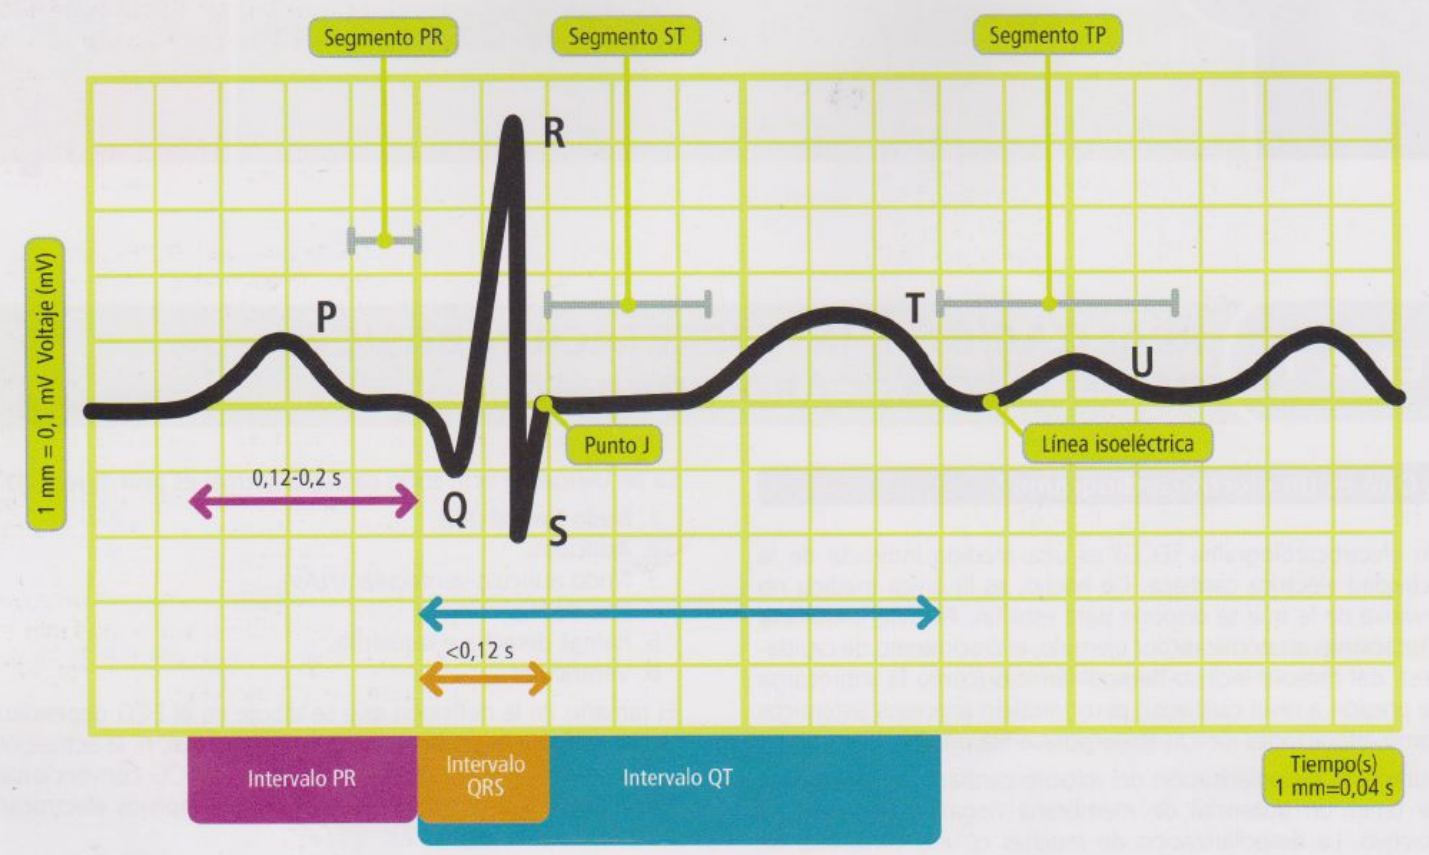
\includegraphics[scale=0.25]{images/teoria_ecg.png}
\end{center}
\caption{Senyal teòrica d'un ECG i els seus segments}
\label{fig: ecg_arduino}
\end{figure}
%
\noindent Hi ha molta literatura que permet identificar malalties analitzant els diferents segments, la seva durada i l'amplitud de la senyal. Tot i que considerem que es podria programar un algorisme per fer un anàlisi de la senyal, ens hem centrat en calcular la freqüència cardíaca amb la fórmula de l'equació \ref{bpm}.
\begin{equation} \label{bpm}
\beta= \frac{1}{T}*1000*60
\end{equation}

\noindent $\beta$: freqüència cardíaca (bpm).\\
$T$: període entre pic i pic (ms).


\section{Rang de freqüència cardíaca habitual}
Una persona al llarg de la seva vida sol tenir una freqüència cardíaca en repòs variable. La medicina no és una ciència exacte i per tant no és d'estranyar que cada autor o referència doni uns nivells habituals de freqüència cardíaca lleugerament diferents.\\
\newline Per donar una referència, la majoria de la població té una freqüència cardíaca que es troba dins l'interval donat a la Taula \ref{tab:consums}:
\begin{table}[H]
\small
  \centering
    \begin{tabu} to \textwidth {|X[4]|X|X|} \hline
     & \multicolumn{2}{|c|}{Freqüència cardíaca (bpm)} \\
    \hline
    \multicolumn{1}{|l}{Edat} & \multicolumn{1}{|l}{Mínim} & \multicolumn{1}{|l|}{Màxim} \\ \hline \hline
    Recent nascuts, de 0 a 1 mes & 70 & 190 \\ \hline
    Bebès de 1 a 11 mesos d'edat & 80 & 160 \\ \hline
    Nens de 1 a 2 anys d'edat  & 80 & 130 \\ \hline
    Nens de 3 a 4 anys d'edat & 80 & 120  \\ \hline
    Nens de 5 a 9 anys d'edat  & 75 & 115 \\ \hline
    Nens a partir de 10 anys i persones adultes & 50 & 100 \\ \hline
    Esportistes amb bon entrenament cardiovascular & 40 & 60 \\ \hline

    \end{tabu}%
  \label{tab:addlabel}%
    \caption{Freqüències cardíaques habituals segons l'edat}
    \label{tab:consums}
\end{table}%

\noindent Com veiem, el rang de freqüència cardíaca és molt gran, especialment durant l'edat adulta. No es pot dir que una persona tingui una malaltia important per tenir el cor a 80 bpm, per exemple. Creiem més important conèixer l'evolució de la freqüència cardíaca d'una persona al llarg de la seva vida que no pas conèixer aquesta magnitud en un instant determinat.\\
\newline És evident que tenir una freqüència cardíaca de 0 bpm o similar indica, sens dubte, que la persona ha patit una parada cardíaca.\\
\newline Es diu que la freqüència cardíaca màxima d'una persona segons la seva edat ve regida per l'equació \ref{beta}.
\begin{equation} \label{beta}
\beta_{opt}=220 - e
\end{equation}

\noindent $e$: edat de la persona (anys).\\

%
%
%
%
%


\section{Electrocardiògrafs actuals i solució proposada}
Tradicionalment un electrocardiograma es podia fer amb un electrocardiògraf analògic, el qual pot ser tant simple com un amplificador diferencial que dona la diferència de tensió entre dos elèctrodes i l'amplifica. La referència d'aquesta tensió pot ser el nivell de tensió d'un tercer elèctrode, el qual actua com a massa.\\
\newline Aquesta configuració de 3 elèctrodes és la que nosaltres escollim, per bé que n'hi ha d'altres de viables que funcionen amb més elèctrodes i que poden ser més fiables.
\begin{figure}[H]
\begin{center}
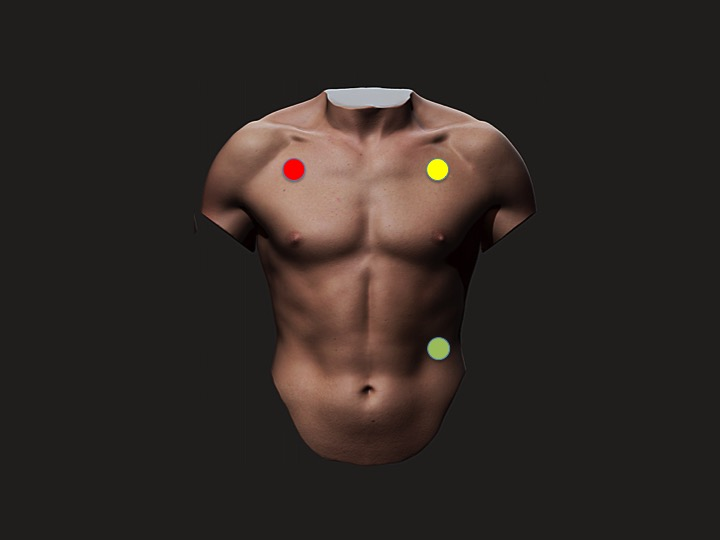
\includegraphics[scale=0.5]{images/electrodos.jpg}
\end{center}
\caption{Col·locació de 3 elèctrodes}
\label{fig: electrodes}
\end{figure}
%ampliar aquí.
%
%
\noindent Un electrocardiògraf analògic no enregistra dades de freqüència cardíaca. Si es desplaça un tros de paper de forma constant i la senyal analògica de tensió s'amplifica adequadament i s'aconsegueix desplaçar de forma proporcional a la tensió llegida una agulla, la qual té un bolígraf o similar a un dels seus extrems amb què pot dibuixar un electrocardiograma.
\begin{figure}[H]
\begin{center}
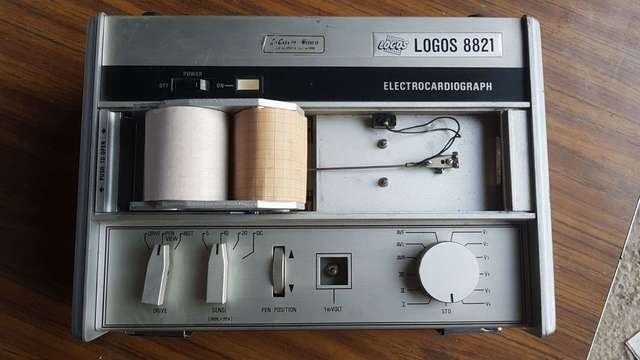
\includegraphics[scale=0.5]{images/ecg.jpg}
\end{center}
\caption{Electrocardiògraf analògic}
\label{fig: electrodes}
\end{figure}
\noindent L'electrònica digital permet estalviar-se dibuixar la senyal de forma analògica sobre un paper. Es basa en mostrejar a alta velocitat la senyal analògica d'entrada i enregistrar les dades. D'aquesta manera es poden representar les dades captades en un pla, donant lloc a l'electrocardiograma.
\begin{figure}[H]
\begin{center}
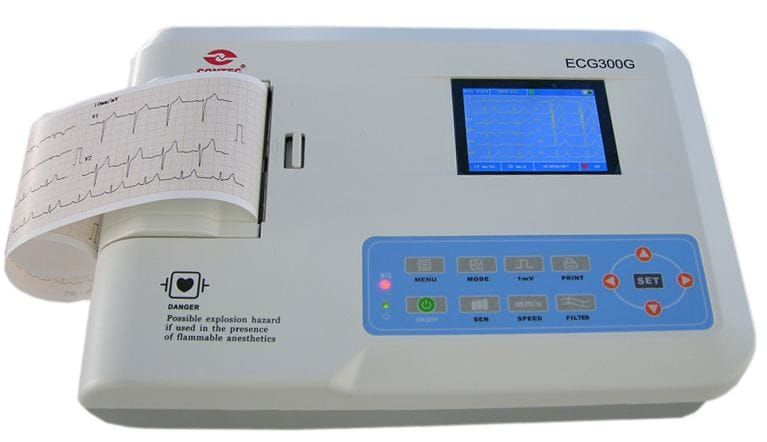
\includegraphics[scale=0.35]{images/ecg_2.jpg}
\end{center}
\caption{Electrocardiògraf actual}
\label{fig: electrodes}
\end{figure}
\noindent Els electrocardiògrafs digitals tenen l'avantatge de poder enregistrar dades, o sigui, tenen memòria. Els electrocardiògrafs analògics no ofereixen aquesta possibilitat. Tot i això, l'equip de la imatge, per exemple, tot i ser digital, funciona com un electrocardiògraf analògic en el sentit de què només imprimeix, no tracta ni emmagatzema de cap manera les dades.\\
\newline Al llarg del treball es mostra com no només es dissenya un electrocardiògraf digital, sinó que aquest guarda dades que són consultables mitjançant una interfície clara, cosa que molts no electrocardiògrafs comercials no fan.\\
\newline Tot i això, també donem l'opció a visualitzar l'electrocardiograma a través del por sèrie de l'Arduino Nano. Mostregem a una freqüència suficient, la qual assegura que no ens perdem cap pic ni cap dada significativa de l'electrocardiograma.
\begin{figure}[H]
\begin{center}
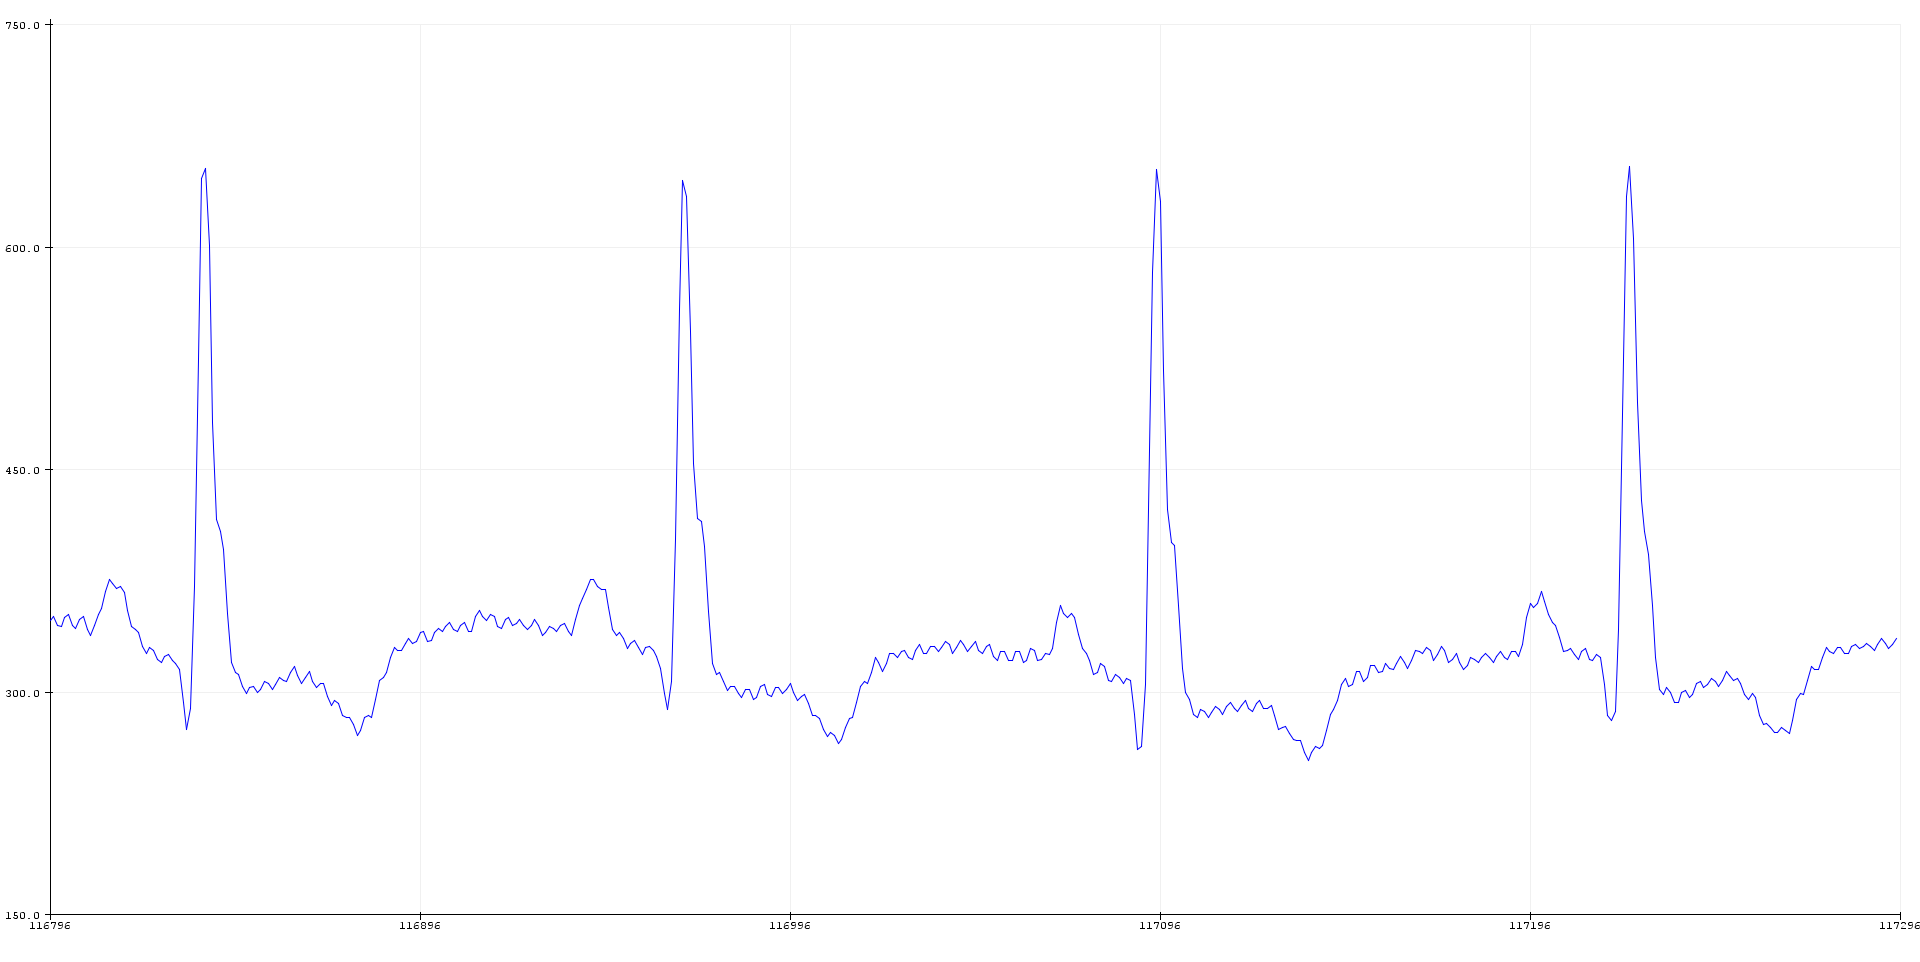
\includegraphics[scale=0.25]{images/ecg_arduino.png}
\end{center}
\caption{Electrocardiògraf donat per l'Arduino}
\label{fig: ecg_arduino}
\end{figure}
%

%





%\chapter{\uppercase{Generador fotovoltaic i inversor}}
Un generador és una màquina, aparell o dispositiu que produeix energia elèctrica amb una tensió i un corrent d'unes característiques determinades. L'adjectiu fotovoltaic s'usa per designar aquells sistemes en què es produeix una força electromotriu entre dos metalls que estan en contacte i exposats a una radiació electromagnètica.\\
\newline Un conjunt de panells solars connectats entre sí ja sigui en sèrie, en paral·lel o amb associació sèrie-paral·lel es pot considerar un sol generador fotovoltaic.\\
\newline Un panell solar ve definit per diferents paràmetres que s'han de tenir en compte a l'hora de dissenyar una instal·lació. Prèviament cal determinar la quantitat de panells de la instal·lació en funció de l'energia que es vol produir.

\section{Potència de la instal·lació fotovoltaica}
S'ha calculat al capítol anterior que el consum total de l'habitatge al cap de l'any és de 5.504 KWh.\\
\newline Es proposa instal·lar les plaques necessàries per generar al cap d'un any un  valor d'energia inferior però proper a l'energia consumida aquell any a l'habitatge. D'aquesta manera hi haurà moments en què tota l'energia elèctrica generada serà igual a la consumida a l'habitatge, altres en què els excedents es lliurin a la xarxa i altres en què les plaques no generin i s'hagi de consumir únicament energia de la xarxa.\\
\newline Es proposa utilitzar un panell amb un eficiència del 17\% i una superfície de 1,94 $m^2$. Amb aquestes dades i coneixent el valor de la irradiació global es determina que un sol panell donarà 517,73 kWh al cap de l'any. 10 panells d'aquest model donaran 5.177 kWh anuals, valor molt proper al d'energia consumida anual a l'habitatge.\\
\newline Cal tenir en compte les ombres generades per l'edifici del costat sud i els arbres d'aquest mateix costat, que tenen una altura superior a la de la casa del projecte. La imatge de la Figura \ref{fig: ombres} s'ha construït a partir de dades reals i a partir de l'IDAE.
\begin{figure}[H]
\begin{center}
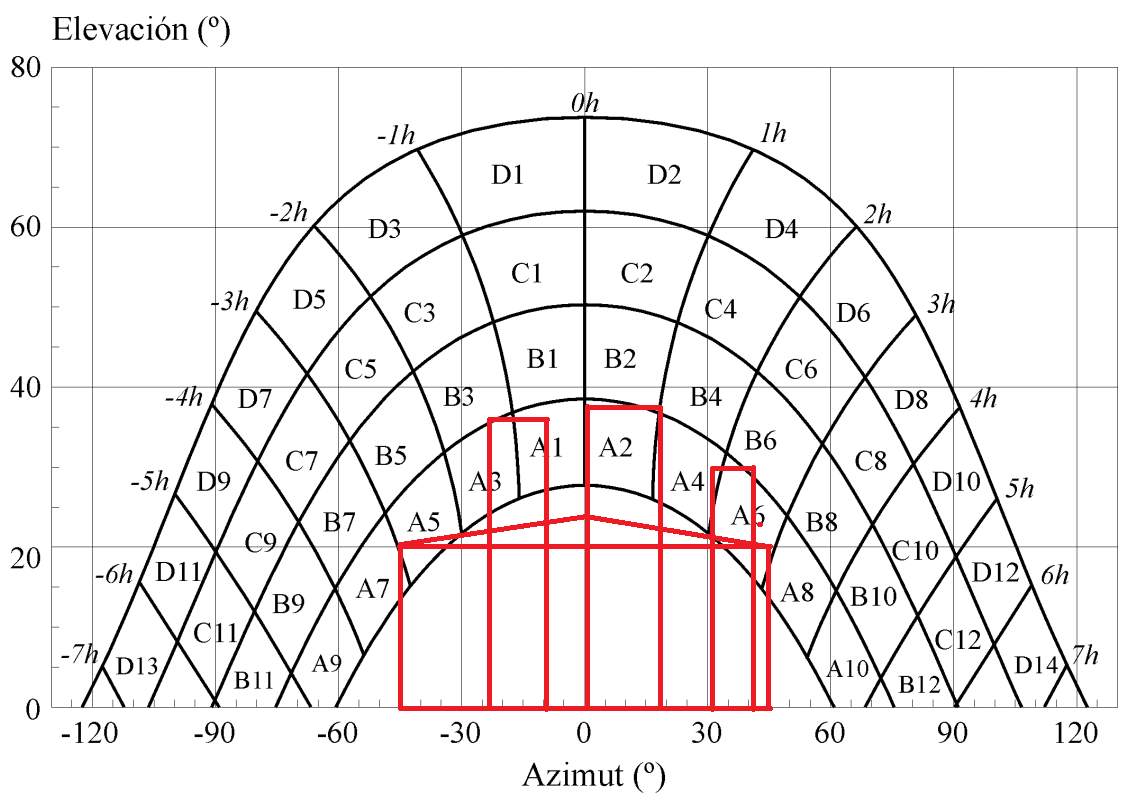
\includegraphics[scale=0.45]{images/o2.png}
\end{center}
\caption{Mapa d'ombres}
\label{fig: ombres}
\end{figure}

\noindent Degut a la inclinació i orientació de les plaques es fa servir la taula 5-A de l'IDAE, per tal de determinar el factor d'ombrejat (FS). Segons l'IDAE cal identificar si cada casella té un 0\%, un 25\%, un 50\%, un 75\% o un 100\% de la seva superfície coberta.\\
\newline La Taula \ref{tab:ombres} mostra el percentatge de superfície de cada casella, el valor de pèrdua tabulat de l'IDAE i la pèrdua que ocasiona cada casella. Així, es dona un total, el factor d'ombrejat (FS).
\begin{table}[H]
\small
  \centering
    \begin{tabular} {|l|r|r|r|}
 \hline  
 \multicolumn{1}{|l|}{Casella} &  \multicolumn{1}{r|}{Factor de superfície} &  \multicolumn{1}{r|}{Sombrejat casella al 100\%} &  \multicolumn{1}{r|}{Sombrejat casella} \\ \hline \hline
A5 & 0,25 & 1,84 & 0,46 \\ \hline
A3 & 0,5 & 2,70 & 1,35 \\ \hline
A1 & 0,5 & 3,15 & 1,58 \\ \hline
A2 & 1,0 & 3,17 & 3,17 \\ \hline
A6 & 0,75 & 1,79 & 1,34 \\ \hline \hline
Total & \multicolumn{3}{r|}{7,90} \\ \hline

    \end{tabular}%
    \caption{Sombrejats}
    \label{tab:ombres}
%\caption{Estances de l'habitatge unifamiliar}
\end{table}%

\noindent El total de 7,9\% entra dins els marges que marca l'IDAE, el qual indica que per instal·lacions de propòsit general el màxim per ombres és del 10\%.\\
\newline El factor d'ombrejat (FS) ve donat per l'Equació \ref{fs}.
\begin{equation} \label{fs}
FS = 1-Perdues \ per \ ombrejat
\end{equation}

\noindent El factor d'ombrejat val 0,921. Per tant, el total d'energia generada al cap de l'any baixa a 4.768 kWh.\\
\newline El factor d'irradiació és 1 perquè es pren l'angle òptim d'inclinació i l'angle d'orientació coincideix amb el sud.

% Per tal de determinar els panells solars escollits, abans necessitem conèixer la radiació que incideix sobre la teulada al llarg de l'any. Per fer-ho es consulta un servei web anomenat Photovoltaic Geographical Information System, de la Comissió Europea. El servei determina que, donades les coordenades de l'habitatge, el més òptim és inclinar les plaques amb un angle de 38$^\circ$ respecte la horitzontal i un angle de -3$^\circ$ respecte l'Azimut.

\section{Panell solar escollit}
El panell solar proposat s'anomena GCL-P6/72. Segons el fabricant és d'alta eficiència ja que pot arribar a tenir un 17\% de rendiment. La seva potència màxima, o potència de pic, és de 330 W. El fabricant indica que el rendiment dels panells disminueix de forma lineal al llarg del temps; al cap de 25 anys s'espera un rendiment d'un 80,7\%.\\
\newline Cal dir que aquests 330 W es poden haver aconseguit en condicions idònies que només es donen al laboratori. El mateix fabricant ens indica que per una irradiació de 800 W/$m^2$ la potència màxima és de 237,71 W.\\
\newline A continuació, a la Taula \ref{tab:panell_ideal}, s'indiquen les característiques elèctriques del panell en condicions idònies, per les quals es dona la potència de 330 W.

\begin{table}[H]
\small
  \centering
    \begin{tabular} {|l|r|}
 \hline  
 \multicolumn{1}{|l|}{Característica del panell GLC-P6/72 330 W, condicions ideals} &  \multicolumn{1}{r|}{Valor} \\ \hline \hline
	Potència màxima ($P_{max}$) & 330,00 W \\ \hline
	Tensió a la potència màxima ($V_m$) & 37,80 V \\ \hline
	Intensitat a la potència màxima ($I_m$) & 8,73 A \\ \hline
	Tensió de circuit obert ($V_{oc}$) & 46,20 V \\ \hline
	Corrent de curtcircuit ($I_{sc}$) & 9,33 A \\ \hline
	Eficiència & 17,00 \% \\ \hline
    \end{tabular}%
    \caption{Dades del panell amb irradiació de 1.000 W/$m^2$ i 25 C$^\circ$ de tempratura ambient}
    \label{tab:panell_ideal}
%\caption{Estances de l'habitatge unifamiliar}
\end{table}%

\noindent En condicions més comunes i no tan ideals la potència disminueix considerablement, com s'indica a la Taula \ref{tab:panell_habitual}.\\
\newline Després de consultar a Internet s'observa que a la zona geogràfica en què es pretén instal·lar les plaques la irradiació pot prendre valors de l'ordre de 800 W/$m^2$ com a màxim. Rebre 1.000 W/$m^2$ no seria gens comú.\\
\newline El mes de novembre, per exemple els pics d'irradiació que es reben són d'uns 600 W/$m^2$.

\begin{table}[H]
\small
  \centering
    \begin{tabular} {|l|r|}
 \hline  
 \multicolumn{1}{|l|}{Característica del panell GLC-P6/72 330 W, condicions no ideals} &  \multicolumn{1}{r|}{Valor} \\ \hline \hline
	Potència màxima ($P_{max}$) & 237,71 W \\ \hline
	Tensió a la potència màxima ($V_m$) & 34,50 V \\ \hline
	Intensitat a la potència màxima ($I_m$) & 6,89 A \\ \hline
	Tensió de circuit obert ($V_{oc}$) & 42,90 V \\ \hline
	Corrent de curtcircuit ($I_{sc}$)& 7,58 A \\ \hline

    \end{tabular}%
    \caption{Dades del panell amb irradiació de 800 W/$m^2$ i 20 C$^\circ$ de tempratura ambient}
    \label{tab:panell_habitual}
%\caption{Estances de l'habitatge unifamiliar}
\end{table}%

\noindent Un altre punt a destacar de la irradiació és que aquesta se sol donar en termes d'energia al cap del dia i no pas de potències. De totes maneres, se seguirà parlant de potències ja que és més pràctic. No s'ha d'oblidar, però, que aquesta potència de 800 W/$m^2$ només es pot donar a l'estiu i en moments de molta irradiació. En les demés hores aquesta potència serà molt menor.

%comentar com es decideix la potència que fa falta
%https://assets.leroymerlin.es/is/content/lmes/82165089-0170q-es/mod-fotovoltaico-gcl-330w.pdf


\section{Associació de plaques} %passar model i tal a annex?
Es decideix associar les plaques amb dues branques de 5 plaques per branca, de manera que es combina l'associació sèrie i paral·lel a la vegada. Per entendre millor aquest apartat es considera important conèixer el model dels panells solars, indicat a la Figura \ref{fig:model}.
\begin{figure}[H]
\begin{center}
\begin{tikzpicture} %http://www.texample.net/media/tikz/examples/TEX/power-electronics-rectifier.tex
    \draw
	(0,0)
	to [I=, l=$I_{PV}$] ++ (0,4)
	(2,4)
	to [D] ++(0,-4)
	(4,0)
	to[R=$R_{sh}$] ++(0,4)

    (0,0) to[short, -o] (7,0)
    (0,4) to[short, current/distance=0.5] (4.5,4)
    to[R=$R_{s}$] (5.5,4)
    to[short, i=$I_{out}$, -o] (7,4)
    
        (8,4)
        to[open, v^=$V_{out}$] ++(0,-4)
;
\end{tikzpicture}
\end{center}
\caption{Model d'un panell solar fotovoltaic}
\label{fig:model}
\end{figure}

\noindent $I_{PV}$: corrent que lliura el mòdul.\\
$R_{sh}$: resistència en paral·lel del panell.\\
$R_{s}$: resistència de contacte del connexionat del panell.\\
$I_{out}$: corrent de sortida.\\
$V_{out}$: tensió de sortida.\\
% 
\newline La corba característica $V_{out}$-$I_{out}$ dels panells solars s'obté d'aquest model i dona una intensitat lineal per un gran rang de tensions de sortida. Per altes tensions de sortida la intensitat de sortida és bastant petita. L'inversor intenta treballar en el punt de màxima potència, anomenat MPPT.\\
\newline Les corbes del panell segons el fabricant són les indicades a la Figura \ref{fig:vi}.
\begin{figure}[H]
\begin{center}
\includegraphics[scale=0.3]{images/corba.png}
\end{center}
\caption{Corbes V-I GLC-P6/72 330 W}
\label{fig:vi}
\end{figure}


\noindent Al connectar diversos panells en sèrie pot passar que algun panell consumeixi energia. Això és molt notori quan hi ha ombres, ja que a algunes plaques els incideix el Sol i lliuren una quantitat considerable d'intensitat mentre que les que estan a l'ombra donen molta menys intensitat. Com que estan connectades en sèrie, la intensitat ha de ser la mateixa. A la placa ombrejada, per tant, li passarà molta intensitat a través de $R_{sh}$. Aquesta resistència té un valor considerable. L'hi poden passar uns quants amperes i pot dissipar potències elevades.\\
\newline En cap cas interessa que un panell consumeixi energia enlloc de generar-ne. Com ja s'ha comentat, a la casa objecte d'aquest projecte s'ha observat que és habitual que es projectin ombres a la teulada, ja sigui pels alts arbres que hi ha properament o per les cases de més alçada que la del projecte.\\
\newline Per solucionar el problema una solució tradicional ha estat connectar díodes en paral·lel als terminals de les plaques. L'inconvenient és que aquests díodes tenen una caiguda de tensió de 0,7 V o 0,4 V si són díodes Schottky. Per una intensitat de branca de 7 A, que es podria donar per les plaques escollides, i considerant que múltiples plaques podrien estar ombrejades, es dissiparia una potència petita però considerable. A més, s'escalfarien els díodes. Aquests díodes es troben dins una petita caixa; l'escalfament els pot arribar a deteriorar i disminuir la robustesa de la instal·lació.\\
\newline Es decideix escollir un díode SM74611, o com diu el fabricant, un díode de derivació intel·ligent. De fet, se'n connectaran sis a cada placa.\\
\newline El panell GLC-P6/72 330 W té 6 files de 12 cel·les cadascuna. S'opta per col·locar un díode en paral·lel amb cada fila. Així, pot haver-hi alguna cel·la ombrejada però la resta del panell pot seguir generant energia.\\
\newline Els díodes SM74611 tenen una caiguda de tensió de 26 mV o menys a 7 A. Es pot afirmar que d'aquesta manera la pèrdua d'energia és mínima. \\
\newline El cost d'un díode és del 2\% aproximadament respecte el del panell.\\
%
%
\newline Un cops justificats els díodes, es poden fer els càlculs per conèixer la tensió i la intensitat màximes de sortides de la instal·lació fotovoltaica a partir de la tensió de circuit obert i a partir de la intensitat de curtcircuit. Aquestes dades es mostren a la Taula \ref{tab:maxs}.

\begin{table}[H]
\small
  \centering
    \begin{tabular} {|l|r|}
 \hline  
 \multicolumn{1}{|c|}{Característica} &  \multicolumn{1}{c|}{Valor} \\ \hline \hline
	Tensió màxima ($V_{max}$) & 256,87 V \\ \hline
	Intensitat màxima per branca & 9,56 A \\ \hline
    \end{tabular}%
%    \caption{Màxims de l'associació sèrie dels panells}
%\caption{Estances de l'habitatge unifamiliar}
\caption{Paràmetres màxims resultants de l'associació de plaques}
\label{tab:maxs}
\end{table}%

\noindent S'ha tingut en compte l'efecte de la temperatura. El fabricant dona uns factors per calcular els pitjors casos. A l'annex de càlculs es detallen.
%Díode SM74611
%http://www.ti.com/lit/ds/symlink/sm74611.pdf

\section{Inversor}

L'inversor escollit és un FRONIUS Primo 3.0-1. És costós en comparació a altres equips amb la mateixa funcionalitat però alhora molt fiable.\\
\newline Seguidament s'adjunta la Taula \ref{tab:inversor} amb algunes de les característiques més rellevants de l'inversor. L'equip és adient per la instal·lació de plaques i l'associació d'aquestes que es proposa. En cap cas se superen els màxims que fixa el fabricant de l'inversor. La potència del Fronius Primo 3.0-1 és correcta per la potència màxima que ens poden donar els panells fotovoltaics.
\begin{table}[H]
\small
  \centering
    \begin{tabular} {|l|r|} \hline
  \multicolumn{1}{|c|}{Característica} &  \multicolumn{1}{c|}{Valor}\\ \hline \hline
	Màxima corrent d'entrada ($I_{dc \ max}$) & 12 / 12 A \\ \hline
	Màxima corrent de curtcircuit & 18 / 18 A \\ \hline
	Rang màxim de tensió d'entrada CC ($U_{cc \ min}$ - $U_{cc \ max}$) & 80 - 1.000 V \\ \hline
	Tensió mínima de posada en marxa ($U_{dc \ arranc}$) & 80 V \\ \hline
	Nombre d'entrades CC & 2 + 2 \\ \hline
	Potència nominal AC ($P_{ac,r}$) & 3.000 W \\ \hline
	Acoblament a la xarxa ($U_{ac,r}$) & 1 NPE 230 V \\ \hline
	
    \end{tabular}%
  \label{tab:addlabel}%
  \caption{Característiques de l'inversor FRONIUS Primo 3.0-1}
  \label{tab:inversor}
 \end{table}%

\noindent Per començar a funcionar l'inversor necessita un mínim de 80 V. Si de dia un o dos panells estan ombrejats i la resta no, l'inversor pot seguir funcionant i lliurant energia.\\
\newline Els rendiments de l'inversor són molt elevats, per un gran rang de treball el rendiment és del 95\% o més. En cap cas el rendiment baixa del 80\%.\\
\newline El fabricant indica que l'inversor intenta donar sempre la màxima potència mitjançant el seu sistema de Dynamic Peak Manager, això vol dir que adapta la seva impedància per fer que el producte de tensió i intensitat sigui màxim.\\
\newline Aquest inversor és fàcil de muntar gràcies a què es pot desmuntar en dues parts: la fixa que va a la paret i és on es realitzen les connexions i la de potència, que pesa 21,5 kg. Primer es munta la part fixa, es realitzen les connexions, i després s'acobla la part de potència.\\
\newline Fronius indica que el Primo 3.0-1 és un equip pensat pel futur, per xarxes elèctriques intel·ligents. Hi ha la possibilitat de comunicar l'inversor per interfícies molt diverses com Modbus RTU, Fronius Solar API, Ethernet...\\
\newline S'opta per connectar l'inversor a Internet mitjançant un cable Ethernet. D'aquesta manera el client podrà visualitzar la generació d'energia elèctrica dels seus panells. La web que ofereix Fronius és entenedora i fàcil d'utilitzar.\\
\newline Gràcies a la web de Fronius i a la web que s'explica al següents capítols el client podrà visualitzar dades dels panells i tenir una molt bona idea de com estan funcionant.\\
\newline L'inversor donarà les dades de tensió, intensitat i potència generada, però no pot saber com està treballant cada panell. Per això hi ha la placa electrònica, la qual llegirà les tensions de cada panell, amb les quals l'usuari podrà determinar si els panells estan ombrejats, curtcircuitats o en funcionament normal.




\clearpage


% Table generated by Excel2LaTeX from sheet 'Hoja1'
%\begin{table}[H]
%  \centering
%    \begin{tabularx} {\textwidth} {|X|r|} \hline
%  \multicolumn{1}{|c|}{Descripció} &  \multicolumn{1}{c|}{Quantitat}\\ \hline \hline
%
 %   Placa GLC 330 W & 10 \\ \hline
%    Inversor FRONIUS Primo 3.0-1 Light 3kW & 1 \\ \hline
%    Metres cable Ethernet RJ-45 CAT 8 & 10 \\ \hline
%    Metres cable 4 m$m^2$ PVC & 45 \\ \hline
 %   Metres cable 1,5 m$m^2$ PVC & 100 \\ \hline
 %   Punteres Enghofer E 4-10, 4 m$m^2$, 10 mm & 20 \\ \hline
 %   Punteres Enghofer E 1.5-10 1,5 m$m^2$ 10 mm & 12 \\ \hline
 %   Cinta aïllant 10 m 1,6 cm & 3 \\ \hline
 %   Caixa estanca Solera CONS 100x100x55 mm & 2 \\ \hline
  %  Canal Euroquint 25,16 mm 1,5 metres & 20 \\ \hline
%    Curva canal VECAMCO & 10 \\ \hline
%    Paquet de 50 brides 200x2,6  mm & 2 \\ \hline
%    Regleta nylon 12 pols 16 mm & 4 \\ \hline
%    Premsaestopes M12 & 10 \\ \hline
%    Cargol autoroscant M4 16 mm & 12 \\ \hline
%    Tacs Fischer 072095 nylon 6x50 mm & 50 \\ \hline
%    Díode SM74611KTTR & 10 \\ \hline
%            Hores enginyer & 1 \\ \hline
%    Hores oficial de primera & 12 \\ \hline
%    Hores oficial de segona & 12 \\ \hline
%    \end{tabularx}%
%  \label{tab:addlabel}%
% \end{table}%

%\chapter{\uppercase{Inversor}}
%Fronius primo 3.0-1, %https://www.fronius.com/es-es/spain/energia-solar/productos/sector-dom%C3%A9stico/inversor/fronius-primo/fronius-primo-3-0-1

L'inversor escollit és un FRONIUS Primo 3.0-1. És costós en comparació a altres inversors però alhora molt fiable. Permet connectar-lo per TCP-IP a la xarxa d'Internet de la casa i així poder consultar en tot moment la quantitat d'energia que la instal·lació de panells solars fotovoltaics genera.\\
Seguidament s'adjunta una taula amb algunes de les característiques més rellevants de l'inversor.
\begin{table}[H]
  \centering
    \begin{tabular} {|l|r|} \hline
  \multicolumn{1}{|c|}{Característica} &  \multicolumn{1}{c|}{Valor}\\ \hline \hline
	Màxima corrent d'entrada ($I_{dc \ max}$) & 12 / 12 A \\ \hline
	Màxima corrent de curtcircuit & 18 / 18 A \\ \hline
	Rang màxim de tensió d'entrada CC ($U_{cc \ min}$ - $U_{cc \ max}$) & 80 - 1.000 V \\ \hline
	Tensió mínima de posada en marxa ($U_{dc \ arranc}$) & 80 V \\ \hline
	Nombre d'entrades CC & 2 + 2 \\ \hline
	Potència nominal AC ($P_{ac,r}$) & 3.000 W \\ \hline
	Acoblament a la xarxa ($U_{ac,r}$) & 1 NPE 230 V \\ \hline
	
    \end{tabular}%
  \label{tab:addlabel}%
  \caption{Característiques de l'inversor FRONIUS Primo 3.0-1}
 \end{table}%

\noindent L'inversor és adient per la instal·lació de plaques i l'associació d'aquestes que es proposa. En cap cas se superen els màxims que fixa el fabricant de l'inversor. La potència de l'inversor és correcta per la potència màxima que ens poden donar els panells fotovoltaics. Per començar a funcionar l'inversor necessita un mínim de 80 V. Si de dia un o dos panells estan ombrejats i la resta no l'inversor pot seguir funcionant i lliurant energia.\\
\newline Els rendiments de l'inversor són molt elevats, per un gran rang de treball el rendiment és del 95 \% o més. En cap cas el rendiment baixa del 80 \%.\\
\newline El fabricant indica que l'inversor intenta donar sempre la màxima potència mitjançant el seu sistema de Dynamic Peak Manager.\\
\newline Fronius permet connectar els seus inversors a Internet amb cable d'Ethernet i amb una aplicació web poder consultar l'energia que han generat i que estan generant les plaques. La interfície és simple i entenedora.\\
\newline Aquest inversor és fàcil de muntar gràcies a què es pot desmuntar en dues parts: la fixa que va a la paret i és on es realitzen les connexions i la de potència, que pesa bastant. Primer es munta la part fixa, es realitzen les connexions, i després s'acobla la part de potència.\\
\newline Fronius indica que el Primo 3.0-1 és un equip pensat pel futur, per xarxes elèctriques intel·ligents. Hi ha la possibilitat de comunicar l'inversor per interfícies molt diverses com Modbus RTU, Fronius Solar API, Ethernet...



\clearpage


% Table generated by Excel2LaTeX from sheet 'Hoja1'
%\begin{table}[H]
%  \centering
%    \begin{tabularx} {\textwidth} {|X|r|} \hline
%  \multicolumn{1}{|c|}{Descripció} &  \multicolumn{1}{c|}{Quantitat}\\ \hline \hline
%
 %   Placa GLC 330 W & 10 \\ \hline
%    Inversor FRONIUS Primo 3.0-1 Light 3kW & 1 \\ \hline
%    Metres cable Ethernet RJ-45 CAT 8 & 10 \\ \hline
%    Metres cable 4 m$m^2$ PVC & 45 \\ \hline
 %   Metres cable 1,5 m$m^2$ PVC & 100 \\ \hline
 %   Punteres Enghofer E 4-10, 4 m$m^2$, 10 mm & 20 \\ \hline
 %   Punteres Enghofer E 1.5-10 1,5 m$m^2$ 10 mm & 12 \\ \hline
 %   Cinta aïllant 10 m 1,6 cm & 3 \\ \hline
 %   Caixa estanca Solera CONS 100x100x55 mm & 2 \\ \hline
  %  Canal Euroquint 25,16 mm 1,5 metres & 20 \\ \hline
%    Curva canal VECAMCO & 10 \\ \hline
%    Paquet de 50 brides 200x2,6  mm & 2 \\ \hline
%    Regleta nylon 12 pols 16 mm & 4 \\ \hline
%    Premsaestopes M12 & 10 \\ \hline
%    Cargol autoroscant M4 16 mm & 12 \\ \hline
%    Tacs Fischer 072095 nylon 6x50 mm & 50 \\ \hline
%    Díode SM74611KTTR & 10 \\ \hline
%            Hores enginyer & 1 \\ \hline
%    Hores oficial de primera & 12 \\ \hline
%    Hores oficial de segona & 12 \\ \hline
%    \end{tabularx}%
%  \label{tab:addlabel}%
% \end{table}%

%\chapter{\uppercase{Instal·lació elèctrica}}
És d'especial importància dimensionar correctament la instal·lació elèctrica dels panells fotovoltaics per tal de complir amb la ITC-BT-40 que tracta sobre instal·lacions generadores de baixa tensió. A més, cal protegir les línies amb les proteccions adients per tal d'evitar malmetre la instal·lació.

\section{Línies elèctriques de la instal·lació fotovoltaica}
La instal·lació elèctrica de la casa s'acull al model d'autoconsum amb compensació d'excedents. Això vol dir que els excedents d'energia, que es lliuren a la xarxa, es paguen a un preu menor al preu de l'energia que consumeix l'habitatge de la xarxa elèctrica. En cap cas, però, el client rebrà diners a cap de mes.\\
\newline A continuació, a la Taula \ref{tab:linies}, s'exposen les diferents línies de què disposa la instal·lació i la longitud més gran de cadascuna. Recordem que a l'inversor li arriben dos parells de cables, cada parell és d'una branca de 5 panells fotovoltaics en sèrie amb els seus díodes com a protecció.

\begin{table}[H]
\small
  \centering
    \begin{tabular} {|l|l|r|} \hline
  \multicolumn{1}{|l|}{Línia} &  \multicolumn{1}{l|}{Descripció} & \multicolumn{1}{c|}{Longitud (m)} \\ \hline \hline
L1 & Connexionat entre els panells solars & 10 \\ \hline
L2 & Connexionat de la branca 1 a l'inversor & 30 \\ \hline
L3 & Connexionat de la branca 2 a l'inversor & 19 \\ \hline
L4 & Connexionat de l'inversor al QGPC & 6 \\ \hline
L5 & Connexionat dels panells fotovoltaics a la placa electrònica & 21 \\ \hline
	
    \end{tabular}%
  \label{tab:addlabel}%
  \caption{Línies de la instal·lació fotovoltaica}
  \label{tab:linies}
 \end{table}%

\noindent La línia de connexionat entre els panells està formada per cables de baixa longitud que sumen els metres indicats a la taula. Hi ha una línia de connexionat dels panells a l'inversor per cada branca. Aquestes línies estan formades per un parell de cables de longituds diferents, i que sumen l'indicat a la taula. La connexió de l'inversor al QGPC es fa amb un parell de cables de la mateix longitud. Hi ha múltiples línies de connexionat dels panells fotovoltaics a la placa electrònica, la línia més llarga té la longitud indicada.\\
\newline Totes les línies són de cables flexibles de coure amb recobriment no propagador d'incendis i opacitat reduïda. Les línies 1, 2 i 4 tenen conductors amb recobriment contra la radiació directa del Sol. La línia 3 usa un cable comú amb recobriment PVC.


\section{Secció dels conductors}
%revisar tubs
Les seccions dels conductors estan calculades per complir amb el REBT. Es detallen els càlculs a l'annex de càlculs. Les seccions proposades es mostren a la Taula \ref{tab:eccions}.
\begin{table}[H]
\small
\begin{center}
 \begin{tabu} to \textwidth {|X[0.4, l]|X[2, l]|X[0.8, r]|X[0.6 , r]|X[0.6 , r]|}%{X | c c c} 
 \hline
 Línia & Descripció & Distància màxima (m) & Seccions ($mm^{2}$) & Diàmetre tub (mm)\\
 \hline \hline 

L1 & Connexionat entre els panells solars &  10 & 2x4 & 16 \\ \hline
L2 & Connexionat de la branca 1 a l'inversor & 30 & 2x10 & 20 \\ \hline 
L3 & Connexionat de la branca 2 a l'inversor  & 19 & 2x6 & 16 \\ \hline 
L4 & Connexionat de l'inversor al QGPC  & 6 & 2x4 + 4 & 25 \\ \hline
L5 & Connexionat dels panells fotovoltaics a la placa electrònica & 21 & 2x1,5 & 32 \\ \hline 

 \end{tabu}
 \caption{Seccions de les línies}
 \label{tab:eccions}
\end{center}
\end{table}

%detallar

\section{Quadre elèctric}
El quadre elèctric de la instal·lació fotovoltaica es troba a l'habitació on hi ha l'inversor i la placa electrònica. Aquesta habitació està situada sota teulada. Al pis de sota, a la planta baixa, hi ha el QGPC.\\
\newline La caixa del petit quadre elèctric que s'instal·larà és el model VE106F, amb un grau IP65.\\
\newline La protecció contra sobreintensitats, situada a la sortida de l'inversor, es mostra a la Taula \ref{tab:sobrei}. S'ha calculat a partir de la tensió de sortida de l'inversor, que és de 230 V, i amb la potència màxima de la instal·lació fotovoltaica, de 3.300 W.

\begin{table}[H]
\small
\begin{center}
 \begin{tabu} to \textwidth {|X[0.4, l]|X[2, l]|X[0.8, r]|X[0.7 , r]|X[0.4 , r]|X[0.4 , r]|}%{X | c c c} 
 \hline
 Línia & Descripció & Intensitat màxima de la línia (A) & Intensitat nominal del PIA (A) & Classe & Pols\\
 \hline \hline 

% L1 & Connexionat entre els panells solars &  10,91 & 16 & C & 2 \\ \hline

L4 & Connexionat de l'inversor al QGPC  & 14,35 & 16 & C & 2 \\ \hline

 \end{tabu}
 \caption{Proteccions contra sobreintensitats}
 \label{tab:sobrei}
\end{center}
\end{table}
%
%
\noindent És necessari disposar d'algun interruptor per obrir els circuits dels panells solars. Es decideix fer-ho amb interruptors magnetotèrmics. La seva intensitat és superior a la de curtcircuit de les plaques. No cal protegir els panells solars contra sobreintensitats, en curtcircuit el seu màxim no supera els 10 A. Els conductors s'han dimensionat per aguantar aquesta intensitat de curtcircuit sense problemes. Els interruptors són els de la Taula \ref{tab:sobrei2}.
%
\begin{table}[H]
\small
\begin{center}
 \begin{tabu} to \textwidth {|X[0.4, l]|X[2, l]|X[0.8, r]|X[0.7 , r]|X[0.4 , r]|X[0.4 , r]|}%{X | c c c} 
 \hline
 Línia & Descripció & Intensitat màxima de la línia (A) & Intensitat nominal del PIA (A) & Classe & Pols\\
 \hline \hline 
L2 & Connexionat de la branca 1 a l'inversor & 9,56 & 16 & C & 2 \\ \hline 
L3 & Connexionat de la branca 2 a l'inversor  & 9,56 & 16 & C & 2 \\ \hline 

 \end{tabu}
 \caption{Interruptors}
 \label{tab:sobrei2}
\end{center}
\end{table}


%revisar
\noindent El dimensionament dels conductors es detalla a l'annex de càlculs, on es tenen en compte els factors de radiació, agrupament, escalfament i el factor de 1,25 que indica la ITC-BT-40. També es té en compte l'efecte de la temperatura sobre les variables dels panells.\\
\newline La protecció contra contactes indirectes ve donada per un diferencial de classe A de 30 mA de sensibilitat, situat a la sortida de l'inversor. Altres característiques s'indiquen a la Taula \ref{tab:ind}.
%

\begin{table}[H]
\small
\begin{center}
 \begin{tabu} to \textwidth {|X[0.3, l]|X[1, l]|X[0.8, r]|X[0.7 , r]|X[0.7 , r]|X[0.4 , r]|}%{X | c c c} 
 \hline
 Línia & Descripció & Intensitat nominal de la línia (A) & Sensibilitat (mA) & Intensitat nominal del diferencial (A) & Classe\\ \hline \hline 

L4 & Connexionat de l'inversor al QGPC  & 14,35 & 30 & 40 & A \\ \hline

 \end{tabu}
 \caption{Proteccions contra contactes indirectes}
 \label{tab:ind}
\end{center}
\end{table}

\noindent Totes les carcasses de les plaques solars, que són metàl·liques, han d'estar connectades al terra de la instal·lació elèctrica de la casa. La resistència de terra es considerarà correcta si la tensió de defecte en qualsevol punt de la casa és menor a 24 V.

\clearpage


% Table generated by Excel2LaTeX from sheet 'Hoja1'
%\begin{table}[H]
%  \centering
%    \begin{tabularx} {\textwidth} {|X|r|} \hline
%  \multicolumn{1}{|c|}{Descripció} &  \multicolumn{1}{c|}{Quantitat}\\ \hline \hline
%
 %   Placa GLC 330 W & 10 \\ \hline
%    Inversor FRONIUS Primo 3.0-1 Light 3kW & 1 \\ \hline
%    Metres cable Ethernet RJ-45 CAT 8 & 10 \\ \hline
%    Metres cable 4 m$m^2$ PVC & 45 \\ \hline
 %   Metres cable 1,5 m$m^2$ PVC & 100 \\ \hline
 %   Punteres Enghofer E 4-10, 4 m$m^2$, 10 mm & 20 \\ \hline
 %   Punteres Enghofer E 1.5-10 1,5 m$m^2$ 10 mm & 12 \\ \hline
 %   Cinta aïllant 10 m 1,6 cm & 3 \\ \hline
 %   Caixa estanca Solera CONS 100x100x55 mm & 2 \\ \hline
  %  Canal Euroquint 25,16 mm 1,5 metres & 20 \\ \hline
%    Curva canal VECAMCO & 10 \\ \hline
%    Paquet de 50 brides 200x2,6  mm & 2 \\ \hline
%    Regleta nylon 12 pols 16 mm & 4 \\ \hline
%    Premsaestopes M12 & 10 \\ \hline
%    Cargol autoroscant M4 16 mm & 12 \\ \hline
%    Tacs Fischer 072095 nylon 6x50 mm & 50 \\ \hline
%    Díode SM74611KTTR & 10 \\ \hline
%            Hores enginyer & 1 \\ \hline
%    Hores oficial de primera & 12 \\ \hline
%    Hores oficial de segona & 12 \\ \hline
%    \end{tabularx}%
%  \label{tab:addlabel}%
% \end{table}%

%\chapter{\uppercase{Quadre elèctric}}
El quadre elèctric de la instal·lació fotovoltaica es troba a l'habitació on hi ha l'inversor i la placa electrònica. Aquesta habitació es troba sota teulada. Al pis de sota, a la planta baixa, es troba el quadre principal (QGPC).\\
\newline El quadre elèctric disposa d'un parell de magnetotèrmics de 2 pols encarregats de protegir la instal·lació dels panells fotovoltaics i permetre desconnectar-los de l'inversor. També hi figura un magnetotèrmic que es troba entre l'inversor i el QGPC.\\
\newline La caixa d'aquest petit quadre elèctric és el model VE106F, amb un grau IP65.

%
%
%

\begin{table}[H]
\small
\begin{center}
 \begin{tabu} to \textwidth {|X[0.4, l]|X[2, l]|X[0.8, r]|X[0.7 , r]|X[0.4 , r]|X[0.4 , r]|}%{X | c c c} 
 \hline
 Línia & Descripció & Intensitat nominal de la línia (A) & Intensitat nominal del PIA (A) & Classe & Pols\\
 \hline \hline 

L1 & Connexionat entre els panells solars &  10,91 & 16 & C & 2 \\ \hline
L2 & Connexionat de la branca 1 a l'inversor & 10,91 & 16 & C & 2 \\ \hline 
L3 & Connexionat de la branca 2 a l'inversor  & 10,91 & 16 & C & 2 \\ \hline 
L4 & Connexionat de l'inversor al QGPC  & 14,35 & 16 & C & 1 \\ \hline

 \end{tabu}
 \caption{Proteccions contra sobreintensitats}
\end{center}
\end{table}


%revisar
\noindent Pel correcte dimensionament de les proteccions contra sobreintensitats s'ha tingut en compte el coeficient de 1,25 que marca el REBT per instal·lacions generadores d'energia. Les plaques com a màxim, en funcionament normal donaran 8,73 A, aplicant el factor estem parlant de 10,91 A.\\
\newline La protecció contra contactes indirectes és un diferencial de classe A de 30 mA de sensibilitat, situat a la sortida de l'inversor.
%

\begin{table}[H]
\small
\begin{center}
 \begin{tabu} to \textwidth {|X[0.3, l]|X[1, l]|X[0.8, r]|X[0.7 , r]|X[0.7 , r]|X[0.4 , r]|}%{X | c c c} 
 \hline
 Línia & Descripció & Intensitat nominal de la línia (A) & Sensibilitat (mA) & Intensitat nominal del diferencial (A) & Classe\\ \hline \hline 

L4 & Connexionat de l'inversor al QGPC  & 14,35 & 30 & 40 & A \\ \hline

 \end{tabu}
 \caption{Proteccions contra contactes indirectes}
\end{center}
\end{table}

\noindent Totes les carcasses de les plaques solars, que són metàl·liques, estan connectades a terra.



\clearpage


% Table generated by Excel2LaTeX from sheet 'Hoja1'
%\begin{table}[H]
%  \centering
%    \begin{tabularx} {\textwidth} {|X|r|} \hline
%  \multicolumn{1}{|c|}{Descripció} &  \multicolumn{1}{c|}{Quantitat}\\ \hline \hline
%
 %   Placa GLC 330 W & 10 \\ \hline
%    Inversor FRONIUS Primo 3.0-1 Light 3kW & 1 \\ \hline
%    Metres cable Ethernet RJ-45 CAT 8 & 10 \\ \hline
%    Metres cable 4 m$m^2$ PVC & 45 \\ \hline
 %   Metres cable 1,5 m$m^2$ PVC & 100 \\ \hline
 %   Punteres Enghofer E 4-10, 4 m$m^2$, 10 mm & 20 \\ \hline
 %   Punteres Enghofer E 1.5-10 1,5 m$m^2$ 10 mm & 12 \\ \hline
 %   Cinta aïllant 10 m 1,6 cm & 3 \\ \hline
 %   Caixa estanca Solera CONS 100x100x55 mm & 2 \\ \hline
  %  Canal Euroquint 25,16 mm 1,5 metres & 20 \\ \hline
%    Curva canal VECAMCO & 10 \\ \hline
%    Paquet de 50 brides 200x2,6  mm & 2 \\ \hline
%    Regleta nylon 12 pols 16 mm & 4 \\ \hline
%    Premsaestopes M12 & 10 \\ \hline
%    Cargol autoroscant M4 16 mm & 12 \\ \hline
%    Tacs Fischer 072095 nylon 6x50 mm & 50 \\ \hline
%    Díode SM74611KTTR & 10 \\ \hline
%            Hores enginyer & 1 \\ \hline
%    Hores oficial de primera & 12 \\ \hline
%    Hores oficial de segona & 12 \\ \hline
%    \end{tabularx}%
%  \label{tab:addlabel}%
% \end{table}%


\chapter{\uppercase{Placa electrònica d'adquisició de dades i comunicació}}
Tal com s'indica als objectius del projecte part del treball consisteix en desenvolupar una placa electrònica encarregada d'adquirir dades, en aquest cas de freqüència cardíaca. \\
\newline Es vol que aquestes dades siguin accessibles i per això s'ha optat per dotar la placa d'un component de comunicació Wi-Fi gràcies al qual es podrà visualitzar una pàgina web amb les dades mesurades.\\
\newline La placa disposa d'una part d'alimentació que s'encarrega d'adaptar les tensions als nivells correctes dels diversos components. Existeix comunicació I2C entre els dos microcontroladors. Un s'encarrega d'adquirir les dades i tractar-les, mentre que l'altre està dedicat a la comunicació Wi-Fi.\\
\newline D'aquesta manera es poden realitzar tasques en paral·lel, cosa que seria impossible de fer amb un sol microcontrolador. Així, el microcontrolador que s'encarrega de la comunicació Wi-Fi pot esta donant servei a un client mentre el microcontrolador de l'Arduino Nano mostreja la senyal analògica.\\
\newline Si s'intentés fer tot amb un sol microcontrolador, podria ser que durant la dècima de segon que es necessita per donar servei al client ens perdéssim un batec. La fiabilitat del sistema disminuïra, i no ho volem.\\
\newline De forma esquemàtica es pot explicar el hardware mitjançant blocs.

\tikzstyle{decision} = [diamond, aspect=2, draw, fill=orange!20, 
    text width=4.5em, text badly centered, node distance=4cm, inner sep=0pt]
\tikzstyle{block} = [rectangle, draw, fill=red!40, 
    text width=5em, text centered, rounded corners, minimum height=5em]
    
\tikzstyle{block2} = [rectangle, draw, fill=green!40, 
    text width=7em, text centered, rounded corners, minimum height=3em, minimum width=7 em]
    
\tikzstyle{punt} = [rectangle, draw, fill=green!40, 
    text width=0em, text centered,  minimum height=0em, minimum width=0 em]
    
\tikzstyle{line} = [draw, -latex']
\tikzstyle{cloud} = [draw, ellipse,fill=red!20, node distance=3cm,
    minimum height=2em]
    
\begin{figure}[H]
\begin{center}
\begin{tikzpicture}[node distance = 2cm, auto, scale=0.65, every node/.style={scale=0.65}]
    % Place nodes
    \node [block] (pila) {Bateria (2,4 V)};  
    \node [block, right of=pila, node distance=5cm] (boost) {Convertidor Boost (5 V)};  
    \node [block, right of=boost, node distance=5cm] (buck) {Convertidor lineal (3,3 V)};  
    
    \node [block2, below of=boost, node distance=4cm] (nano) {Arduino Nano}; 
    \node [block2, left of=nano, node distance=6cm] (anell) {Anell de LEDs}; 
    \node [block2, below of=buck, node distance=4cm] (esp) {ESP-01}; 
    \node [block2, right of=esp, node distance=6cm] (ad8232) {AD8232};        

    % Draw edges
    \path [line] (pila) -- node [above] {2,4 V} (boost);
    \path [line] (boost) -- node [above] {5 V} (buck);
    
    \path [line] (boost) -- node [right] {5 V} (nano);
    \path [line] (boost) -- node [left] {5 V} (anell);
    \path [line] (buck) -- node [right] {3,3 V} (esp);
    \path [line] (buck) -- node [right] {3,3 V} (ad8232);
    
    \path [line] (nano) -- node [above] {DMX} (anell);
    \path [line] (nano) -- node [above] {bpm} (esp);
    

    \draw [->] (ad8232) to[bend left] node[auto] {Senyal analògica} (nano);
        
\end{tikzpicture}
\end{center}
\caption{Esquema de blocs del hardware}
\label{fig:organigrama}
\end{figure}

\section{Alimentació}
% Comentar com s'aliment placaa la. Afegir l'equip a amidaments i pressupost.
L'etapa de potència del nostre equip s'encarrega de transformar la tensió d'aproximadament 2,4 V de dues piles en sèrie a 5 V mitjançant un convertidor Boost que admet una tensió d'entrada mínima de 1 V i pot donar fins a 500 mA a la seva sortida de 5 V. Té una eficiència elevada i la seva sortida és constant. Les dimensions són acceptables.
\begin{figure}[H]
\begin{center}
\includegraphics[scale=0.25]{images/5V.jpg}
\end{center}
\caption{Regulador de tensió 5 V}
\label{fig: 5v}
\end{figure}
\noindent Algunes característiques del regulador són les indicades a la Taula \ref{tab:regulador}.
\begin{table}[H]
\small
\begin{center}
 \begin{tabular} {|l|r|}%{X | c c c} 
 \hline
 Característica & Valor \\
 \hline \hline 
Tensió de sortida & 5 V \\ \hline
Corrent màxim de sortida & 500 mA\\ \hline
Tensió mínima d'entrada & 1 V \\ \hline
Precisió de regulació de voltatge & 1\% \\ \hline
Tensió màxima d'entrada & 5 V \\ \hline
Topologia & Boost, font commutada \\ \hline
 \end{tabular}
 \caption{Característiques del regulador de tensió de la pila}
 \label{tab:regulador}
\end{center}
\end{table}
%\si\ohm
\noindent No n'hi ha prou de tenir 5 V a la sortida d'aquest convertidor. Els 5 V són necessaris per alimentar l'Arduino Nano, ja que el seu microcontrolador ATMEGA328 funciona a 5 V. La petita placa que conté l'ESP8266 i la placa de l'ADS8232 van alimentades a 3,3 V. Per tant, és necessari disposar d'una tensió d'alimentació de 3,3 V.\\
\newline El més directe seria fer servir el pin de 3,3 V de l'Arduino Nano, però comportaria un gran perill per aquesta placa de desenvolupament. Els 3,3 V de l'Arduino Nano venen d'un pin del mateix xip ATMEGA328. La màxima intensitat de sortida que pot donar és de 50 mA. El component ESP8266 consumeix, en funcionament normal, uns 70 mA, així que no és una solució.\\
\newline S'opta per un regulador lineal de bona eficiència anomenat AMS1117-3.3. Està especialment pensat per passar de tensions de 5 V a 3,3 V, que és exactament el que necessitem. A la seva entrada hi connectarem un condensador de 10 uF, així com a la seva sortida. Aquests condensadors evitaran la caiguda de tensió a la sortida en pics d'intensitat a la sortida.\\
\newline S'ha escollit aquest component amb el package SMD per tal d'optimitzar al màxim l'espai.
\begin{figure}[H]
\begin{center}
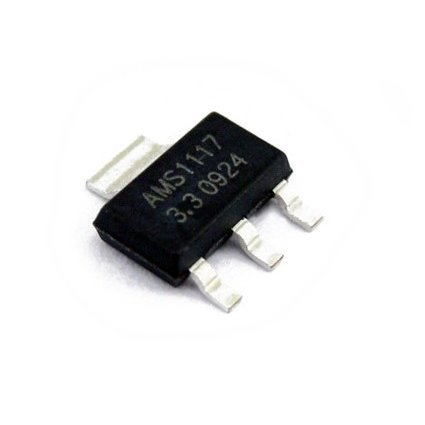
\includegraphics[scale=0.35]{images/ams3v3.jpg}
\end{center}
\caption{Regulador de tensió 3,3 V AMS1117 3,3}
\label{fig: 3v3}
\end{figure}
%
%
\noindent Algunes característiques del regulador són les indicades a la Taula \ref{tab:regulador2}.
\begin{table}[H]
\small
\begin{center}
 \begin{tabular} {|l|r|}%{X | c c c} 
 \hline
 Característica & Valor \\
 \hline \hline 
Tensió de sortida & 3,3 V \\ \hline
Corrent màxim de sortida & 800 mA\\ \hline
Tensió d'entrada & 5 V \\ \hline
Precisió de regulació de voltatge & 1,4\% \\ \hline
Topologia & Lineal \\ \hline
 \end{tabular}
 \caption{Característiques del regulador de tensió de 5 V a 3,3 V}
 \label{tab:regulador2}
\end{center}
\end{table}
%
\noindent Noteu els 800 mA màxims de sortida. Si considerem que la placa amb l'ESP8266 pot arribar a, com a màxim, pics de 200 mA i que la placa d'instrumentació té consums habituals de 170 uA (si no es considera el LED que pot tenir en alguns models comercials), no hi ha dubte que aparentment no hi ha problemes.\\
\newline En resum, podem mostrar una imatge que il·lustra de forma bastant intuïtiva les connexions d'aquests equips d'alimentació. Permeten adaptar la tensió de la pila als diferents nivells que requereixen les diferents plaques.
\begin{figure}[H]
\begin{center}
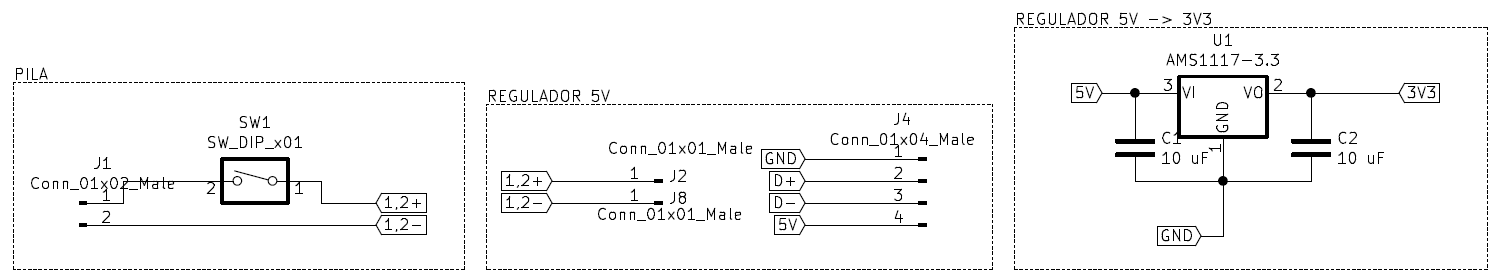
\includegraphics[scale=0.30]{images/alimentacio_2.png}
\end{center}
\caption{Etapes de potència de l'equip}
\label{fig:alimentacio}
\end{figure}

\section{Instrumentació}
% Insistir en la part d'instrumentació, posar equacions i indicar càlculs seguits
% Discutir per què s'ha escollit un OP AMP o un altre i així
La part d'instrumentació de la placa dona una senyal analògica a partir de la senyal captada als tres elèctrodes. Per això es fa servir una placa de desenvolupament que conté un integrat anomenat AD8232.

\begin{figure}[H]
\begin{center}
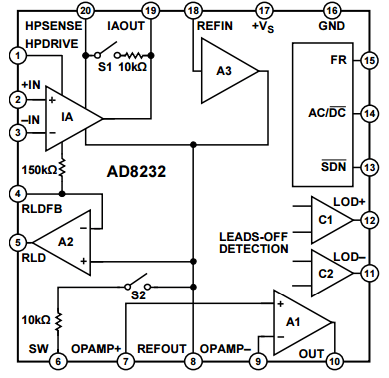
\includegraphics[scale=0.50]{images/ad8232_blocs.png}
\end{center}
\caption{Diagrama de blocs de l'integrat AD82332}
\label{fig:ad8232}
\end{figure}
%
%
\noindent En essència, el que es fa és alimentar la placa i llegir les tensions als tres elèctrodes. Dues d'aquestes tensions es resten i el resultat s'amplifica amb un amplificador diferencial, la referència del qual és el tercer elèctrode.

\begin{figure}[H]
\begin{center}
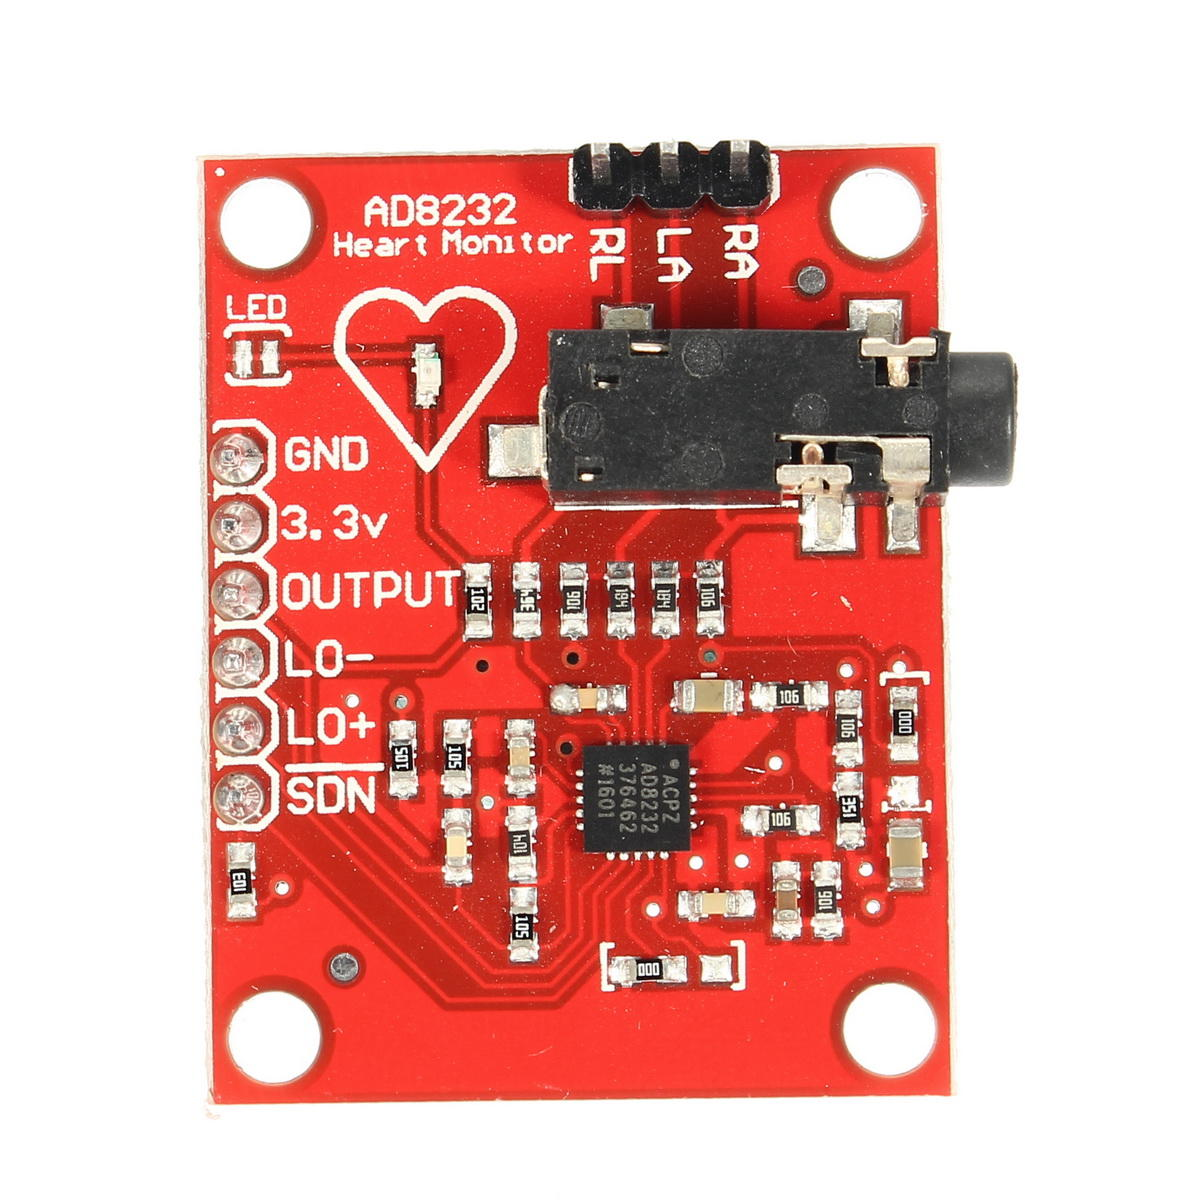
\includegraphics[scale=0.3]{images/ad8232.jpg}
\end{center}
\caption{AD8232 en una placa de desenvolupament}
\label{fig:ad8232}
\end{figure}
%
\noindent La sortida analògica de la placa que mostrem és fruit de les 3 tensions, tal com acabem d'explicar. Si les limitacions d'espai no fossin un problema es podria haver afegit un filtre pas baix per eliminar la freqüència de 50 Hz, provinent de la xarxa elèctrica.

\section{Anell de LEDs}
S'ha previst disposar d'un anell de LEDs per visualitzar de forma ràpida i intuïtiva la freqüència cardíaca de la persona que porti el dispositiu. Per bé que no podrà conèixer amb excessiva precisió la freqüència cardíaca de la persona, se'n pot fer una bona idea.\\
\newline L'anell que s'ha escollit és de la casa SparkFun. Té 16 LEDs 5050 disposats de forma circular. S'ha d'alimentar a 5 V i mitjançant un pin de DATA\_IN es pot fer el control dels colors de tots els LEDs així com de la seva intensitat llumínica i la seva saturació.\\
\newline Sparkfun té les seves llibreries com a codi obert, de forma que és molt fàcil testejar exemples i entendre de forma pràctica com funcionen.

\begin{figure}[H]
\begin{center}
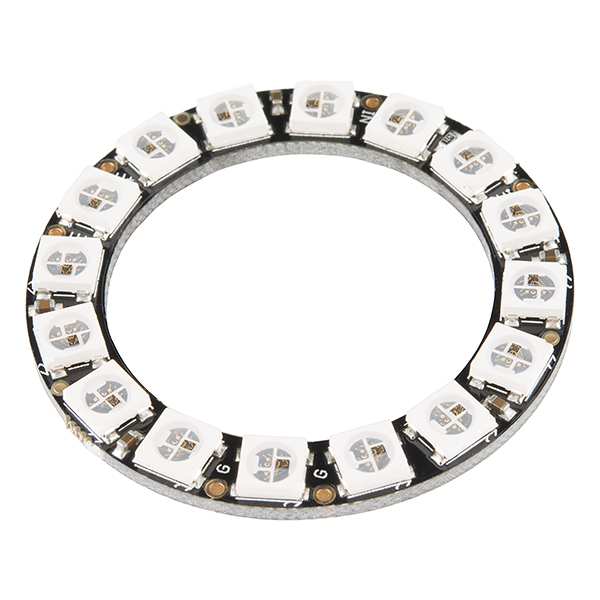
\includegraphics[scale=1.5]{images/led_ring.jpg}
\end{center}
\caption{Anell de LEDs}
\label{fig:ledring}
\end{figure}
%
\noindent La programació de l'anell s'ha fet de manera que cada LED té un color determinat. Si la freqüència és igual o més alta a la freqüència que simbolitza aquell LED, aquest s'encén. En cas contrari s'apaga. Cada vegada que hi ha un pols es fa com un refresc o "barrido" i s'encenen tants LEDs com cal. D'aquesta manera es dona una sensació de dinamisme.\\
\newline El consum d'aquest anell és de 18 mA segons indica el fabricant. Hem pogut comprovar que aquest número s'ajusta molt al mesurat a la realitat, i ens va sorprendre que fos així, ja que de normal un LED d'aquest tipus consumeix cap a uns 20 mA en funcionament normal.\\
\newline La raó que explica com és que el consum de 16 LEDs il·luminats a la vegada sigui tan baix és que cada LED s'il·lumina durant molt poc temps. Això es fa a alta freqüència i per tant l'ull humà ho interpreta com si cada LED sempre estigués encès.

\section{Comunicació}
% Explicar els diferents blocs lògics de la placa
L'ESP8266 permet establir comunicació Wi-Fi de forma efectiva. Després de fer algunes proves hem pogut determinar que el rang de comunicació possible de l'ESP8266 és proper al d'un telèfon mòbil convencional. La seva antena és una pista de circuit imprès. Actualment els mòbils també utilitzen aquest tipus d'antena.\\
\newline L'integrat ESP8266 muntat en una placa amb antena, cristall oscil·lador, resistències de pullup i condensadors de desacoblament es coneix com a ESP-01 i el seu pinout.
\begin{figure}[H]
\begin{center}
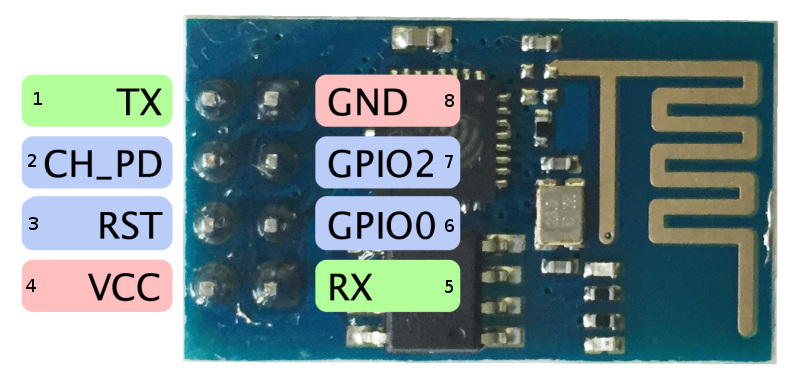
\includegraphics[scale=0.4]{images/esp01.jpg}
\end{center}
\caption{ESP-01}
\label{fig:ledring}
\end{figure}
%
\noindent El fet de què aquesta placa només tingui 8 pins no vol dir que el component només tingui 8 pins, de fet en té al voltant de 30. La placa que utilitzem té dos pins d'alimentació, un pin de TX i un de RX, dos pins de caràcter general, un pin per fer reset i un pin per habilitar l'integrat.\\
\newline El fabricant indica que es deixi una àrea lliure de coure sota l'antena per evitar interferències i problemes de comunicació.\\
\newline Algunes característiques de l'ESP8266 venen donades a la Taula \ref{tab:ESP8266}.
\begin{table}[H]
\small
\begin{center}
 \begin{tabular} {|l|r|}%{X | c c c} 
 \hline
 Característica & Valor \\
 \hline \hline 
Certificació & Wi-Fi Alliance \\ \hline
Freqüència de treball & 2,4 GHz \\ \hline
Potència de l'emissor & 17 dBm \\ \hline
Llindar de potència del receptor & -75 dBm \\ \hline
Rang de tensió d'alimentació & 2,5 V a 3,6 V \\ \hline
Corrent en funcionament normal & 80 mA \\ \hline

 \end{tabular}
 \caption{Característiques de l'integrat de comunicació ESP-8266}
 \label{tab:ESP8266}
\end{center}
\end{table}
% \si\ohm

\noindent D'aquí la importància d'alimentar-lo amb 3,3 V enlloc dels 5 V que ens arriben a la sortida del primer regulador. Per això es fa servir el regulador de tensió que passa de 5 V a 3,3 V.\\
\newline Un altre aspecte a destacar és la tensió dels pins digitals. En el nostre cas s'estableix comunicació I2C entre l'ESP-01 i l'Arduino Nano. Els pins digitals de l'Arduino Nano treballen a 5 V i els de l'ESP-01 en principi estan pensats per treballar a 3,3 V, que és la seva tensió d'alimentació. Així, podria haver-hi problemes si no es fes servir un adaptador de tensions. El fabricant de l'ESP-01, però, ja va preveure que podria haver-hi conflicte i assegura que els pins digitals poden estar a 5 V sense problema de danyar l'integrat.

\section{Circuit imprès}
% Questions de PCB, clearance i tal
S'ha dissenyat un PCB a doble cara que conté les parts electròniques que s'han anat comentant.\\
\newline Per bé que es podria haver ajuntat els esquemàtics de totes les plaques d'avaluació que fem servir en una sola placa de circuit imprès, això hauria portat un temps considerable per adquirir tots els components i testejar-los. A més, alguns components ens hauria sigut molt difícil, per no dir impossible, de soldar manualment.\\
\newline Si aquest projecte seguís endavant i tingués el finançament necessari, llavors sens dubte s'optaria per contractar un servei integral en què ens fessin el PCB i ens hi soldessin els components.\\
%
%
%
\newline Les pistes d'alimentació s'han fet més gruixudes que les de senyal digital. Les pistes de tensió de les plaques s'han fet una mica més gruixudes, tot i que la intensitat a través seu és petita. La separació d'una d'aquestes pistes amb la resta és generosa per evitar l'arc elèctric. A més, es preveu recobrir la placa amb una pel·lícula, cosa que disminuiria encara més el risc d'arc elèctric.\\
\newline La majoria de components són SMD. Solen ser més barats i ocupen molt menys espai en comparació als components que travessen la placa. Així, les dimensions finals de la placa són de 4,5 x 4,1 cm aproximadament.\\
\newline S'han seguit especificacions del fabricant pel disseny de la part de RF. Pel disseny de la part d'instrumentació s'ha tingut especial cura en utilitzar condensadors de desacoblament a les alimentacions dels integrats i situar-los prop d'aquests.\\
\newline La vista superior de com quedaria la placa és la de la Figura \ref{fig:3d_sup}.
\begin{figure}[H]
\begin{center}
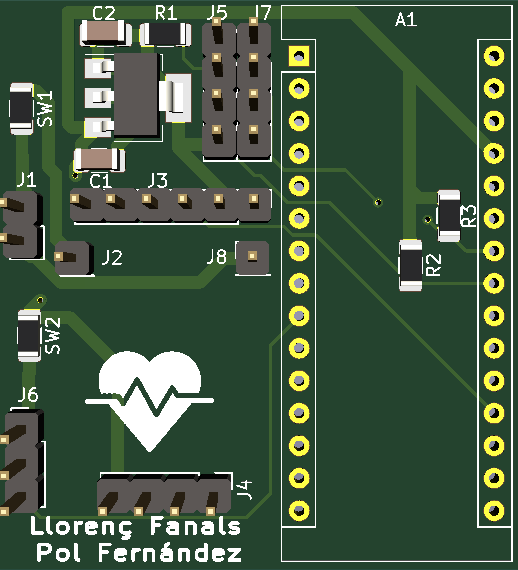
\includegraphics[scale=0.4]{images/placa.png}
\end{center}
\caption{Vista 3D de la cara superior de la placa}
\label{fig:3d_sup}
\end{figure}

\noindent No es disposa del model 3D de l'Arduino Nano.\\
\newline Es pot observar com figuren una gran quantitat de connectors. La majoria simbolitzen allà on aniran connectades les plaques de desenvolupament. Algunes aniran amb pins de gran longitud per aconseguir tenir, a part d'aquesta placa "base", dos nivells més de plaques.\\
\newline D'aquesta manera s'intenta optimitzar l'espai el màxim possible. Si es col·loquessin totes les plaques de desenvolupament de costat el resultat seria un equip amb molt poc gruix però molta superfície.\\
\newline La serigrafia de què s'ha dotat la placa facilita les connexions de les diferents plaques de desenvolupament.\\
\newline Pel que fa a la cara inferior, aquesta es mostra a la Figura \ref{fig:inf}. Aquesta cara s'utilitza per fer passar alguna pista que d'altra manera congestionaria la cara superior. Per passar d'una capa a l'altra es fan servir via's. La resta de la cara superior conté el pla de massa i forats pels components through-hole.

\begin{figure}[H]
\begin{center}
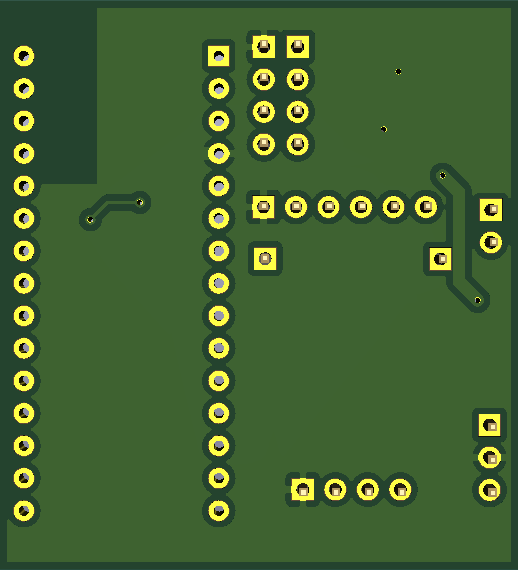
\includegraphics[scale=0.4]{images/placa2.png}
\end{center}
\caption{Vista de la cara inferior de la placa}
\label{fig:inf}
\end{figure}
\noindent Hem decidit encarregar aquesta placa a Xina. Per uns 20 € hem aconseguit 5 unitats i amb transport ràpid. El fabricant, JLCPCB, ha fabricat la placa en menys de 24 hores. L'enviament ha durat uns 3 dies. Considerem el resultat molt satisfactori:
\begin{figure}[H]
\begin{center}
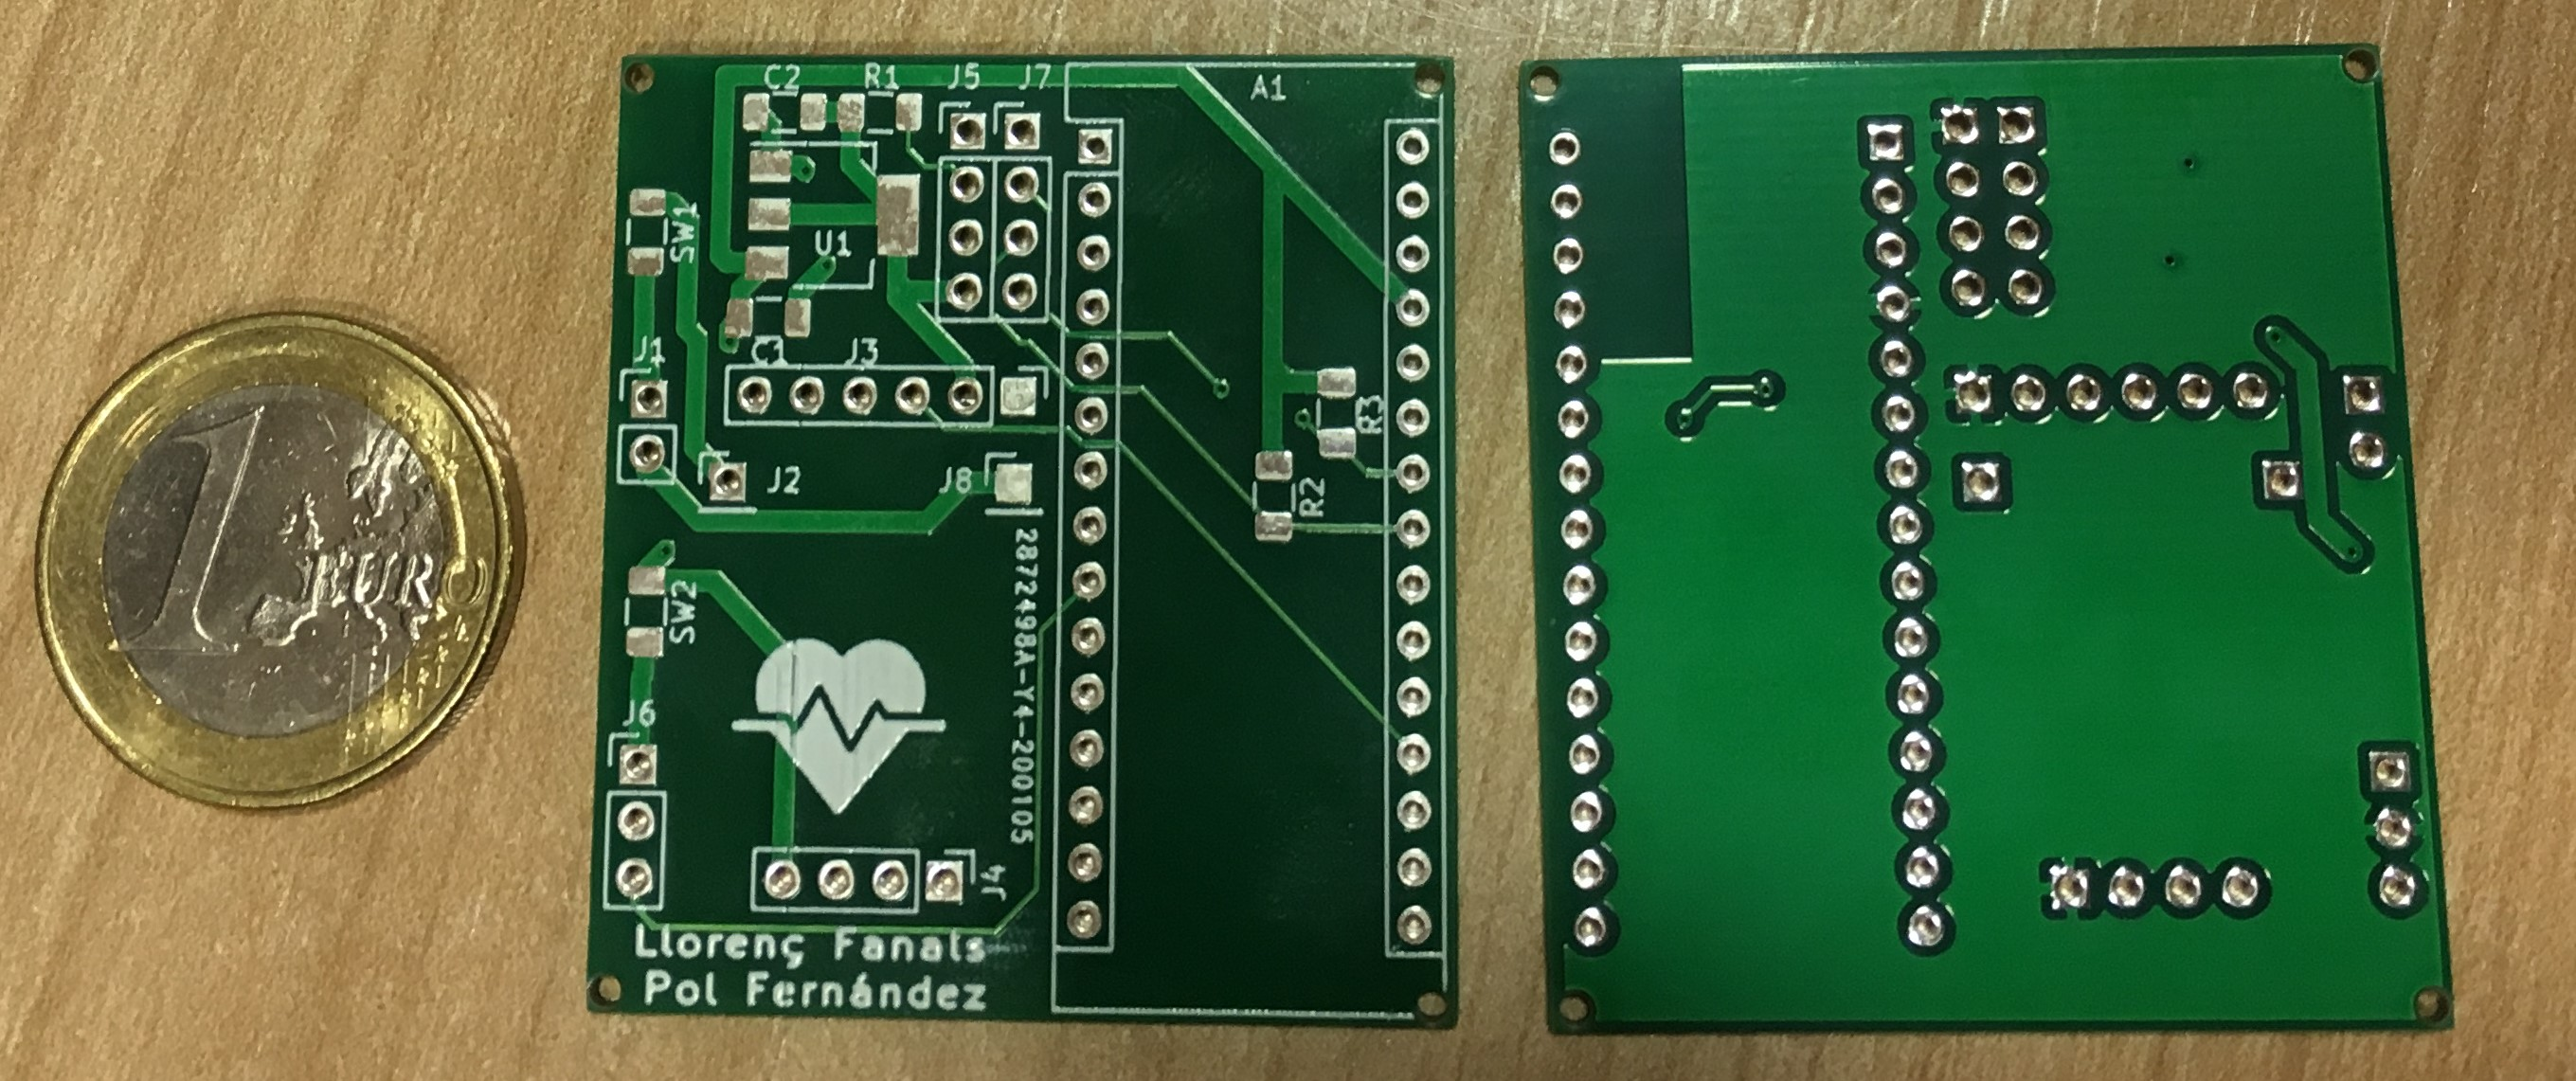
\includegraphics[scale=0.15]{images/pcb_fisic.jpg}
\end{center}
\caption{Vista de les dues cares del PCB}
\label{fig:inf}
\end{figure}

\clearpage


% Table generated by Excel2LaTeX from sheet 'Hoja1'
%\begin{table}[H]
%  \centering
%    \begin{tabularx} {\textwidth} {|X|r|} \hline
%  \multicolumn{1}{|c|}{Descripció} &  \multicolumn{1}{c|}{Quantitat}\\ \hline \hline
%
 %   Placa GLC 330 W & 10 \\ \hline
%    Inversor FRONIUS Primo 3.0-1 Light 3kW & 1 \\ \hline
%    Metres cable Ethernet RJ-45 CAT 8 & 10 \\ \hline
%    Metres cable 4 m$m^2$ PVC & 45 \\ \hline
 %   Metres cable 1,5 m$m^2$ PVC & 100 \\ \hline
 %   Punteres Enghofer E 4-10, 4 m$m^2$, 10 mm & 20 \\ \hline
 %   Punteres Enghofer E 1.5-10 1,5 m$m^2$ 10 mm & 12 \\ \hline
 %   Cinta aïllant 10 m 1,6 cm & 3 \\ \hline
 %   Caixa estanca Solera CONS 100x100x55 mm & 2 \\ \hline
  %  Canal Euroquint 25,16 mm 1,5 metres & 20 \\ \hline
%    Curva canal VECAMCO & 10 \\ \hline
%    Paquet de 50 brides 200x2,6  mm & 2 \\ \hline
%    Regleta nylon 12 pols 16 mm & 4 \\ \hline
%    Premsaestopes M12 & 10 \\ \hline
%    Cargol autoroscant M4 16 mm & 12 \\ \hline
%    Tacs Fischer 072095 nylon 6x50 mm & 50 \\ \hline
%    Díode SM74611KTTR & 10 \\ \hline
%            Hores enginyer & 1 \\ \hline
%    Hores oficial de primera & 12 \\ \hline
%    Hores oficial de segona & 12 \\ \hline
%    \end{tabularx}%
%  \label{tab:addlabel}%
% \end{table}%

%\chapter{\uppercase{Caixa}}




\clearpage


% Table generated by Excel2LaTeX from sheet 'Hoja1'
%\begin{table}[H]
%  \centering
%    \begin{tabularx} {\textwidth} {|X|r|} \hline
%  \multicolumn{1}{|c|}{Descripció} &  \multicolumn{1}{c|}{Quantitat}\\ \hline \hline
%
 %   Placa GLC 330 W & 10 \\ \hline
%    Inversor FRONIUS Primo 3.0-1 Light 3kW & 1 \\ \hline
%    Metres cable Ethernet RJ-45 CAT 8 & 10 \\ \hline
%    Metres cable 4 m$m^2$ PVC & 45 \\ \hline
 %   Metres cable 1,5 m$m^2$ PVC & 100 \\ \hline
 %   Punteres Enghofer E 4-10, 4 m$m^2$, 10 mm & 20 \\ \hline
 %   Punteres Enghofer E 1.5-10 1,5 m$m^2$ 10 mm & 12 \\ \hline
 %   Cinta aïllant 10 m 1,6 cm & 3 \\ \hline
 %   Caixa estanca Solera CONS 100x100x55 mm & 2 \\ \hline
  %  Canal Euroquint 25,16 mm 1,5 metres & 20 \\ \hline
%    Curva canal VECAMCO & 10 \\ \hline
%    Paquet de 50 brides 200x2,6  mm & 2 \\ \hline
%    Regleta nylon 12 pols 16 mm & 4 \\ \hline
%    Premsaestopes M12 & 10 \\ \hline
%    Cargol autoroscant M4 16 mm & 12 \\ \hline
%    Tacs Fischer 072095 nylon 6x50 mm & 50 \\ \hline
%    Díode SM74611KTTR & 10 \\ \hline
%            Hores enginyer & 1 \\ \hline
%    Hores oficial de primera & 12 \\ \hline
%    Hores oficial de segona & 12 \\ \hline
%    \end{tabularx}%
%  \label{tab:addlabel}%
% \end{table}%

\chapter{\uppercase{Programació}}
% Testejar cosetes i poder treure algun screenshot (?, o l'screen shot no fa falta?
% Adjuntar codi, aquí o en annex
Tot el hardware explicat anteriorment ha d'anar recolzat del seu software. En aquest cas, el més primordial és mostrejar la senyal analògica per tal de poder determinar si aquesta supera un llindar de màxim o si disminueix d'un llindar de mínim. Això ho fa l'Arduino Nano, la qual disposa d'entrades analògiques.\\
\newline En segon lloc cal que l'Arduino Nano controli els LEDs i n'encengui més o menys en funció de la freqüència cardíaca mesurada.\\
\newline Mostrar la pàgina web se n'encarrega l'ESP-01, i hem comprovat que requereix d'uns 100 ms per fer-ho. La resta del temps es dedica a sol·licitar dades a l'Arduino Nano. Si aquesta no té cap nova dada de freqüència cardíaca per enviar, simplement no diu res. 


\section{Organigrama Arduino Nano}
L'organigrama de la Figura \ref{fig:organigrama2} ens permet entendre a alt nivell el funcionament del programa que s'encarrega de llegir la tensió analògica provinent de l'ADS8232, calcular la freqüència cardíaca, controlar els LEDs i passar la freqüència cardíaca. A l'annex de programa figura el codi complet.


% fill=blue!20, 
\tikzstyle{decision} = [diamond, draw, fill=orange!30, 
    text width=4.5em, text badly centered, node distance=3cm, inner sep=0pt]
\tikzstyle{block} = [rectangle, draw, fill=blue!20, 
    text width=5em, text centered, rounded corners, minimum height=4em]
\tikzstyle{line} = [draw, -latex']
\tikzstyle{cloud} = [draw, ellipse,fill=red!20, node distance=3cm,
    minimum height=2em]
    
\begin{figure}[H]
\begin{center}
\begin{tikzpicture}[node distance = 3cm, auto, scale=0.8, every node/.style={scale=0.8}]
    % Place nodes
    \node [block] (inici) {\footnotesize Inicialització};
    \node [block, text width=4cm, minimum height = 1cm, inner sep=0pt, below of=inici, node distance=2.5cm] (lectura) {\footnotesize Lectura entrada analògica};
 \node [decision, right of=lectura, node distance=4cm] (max) {\footnotesize $Lectura > llindar\_max ?$};
 \node [decision, left of=lectura, node distance=4cm] (min) {\footnotesize $Lectura < llindar\_min ?$};  
    \node [block, below of=max, minimum height = 1cm, inner sep=0pt, minimum width=5cm, text width=5cm, node distance=3cm] (bloc_max) {\footnotesize $memoria\_temps = millis();$   $flag = 1;$};  
    \node [block, minimum width=5cm, text width=4.5cm, minimum height = 1cm, inner sep=0pt, below of=bloc_max, node distance=2cm] (accio_pic) {\footnotesize $calcul\_bpm(); disponible = 1;$};    
    \node [block, node distance=2cm, minimum width=5cm, text width=4.5cm, minimum height = 1cm, inner sep=0pt, below of=accio_pic, node distance=2cm] (apaga) {\footnotesize Apaga LEDs}; 
        
    \node [block, minimum width=5cm, text width=4.5cm, minimum height = 1cm, inner sep=0pt, below of=min, node distance=3cm] (bloc_min) {\footnotesize $flag = 0;$}; 
    
\node [block, node distance=6cm, minimum width=5cm, text width=4.5cm, minimum height = 1cm, inner sep=0pt, below of=bloc_min] (leds) {\footnotesize $Encendre \ LED == true \ ? \ encen\_LED :$}; 
    
   %Encendre LED == true ? encen_LED :
    
%        \node [ left of=wifi, node distance=4cm] (punt) {.};

    % Draw edges
    \path [line] (inici) -- (lectura);
    \path [line] (lectura) -- (max);
    \path [line] (lectura) -- (min);
    
    \path [line] (max) -- (bloc_max);
    \path [line] (bloc_max) -- (accio_pic);
    \path [line] (accio_pic) -- (apaga);
    
    \path [line] (min) -- (bloc_min);
    
    \path [line] (bloc_min) -- (leds);
    \path [line] (apaga) -- (leds);

     \draw [->] (leds) to[out=170, in=135] node[auto] {} (inici);
\end{tikzpicture}
\end{center}
\caption{Organigrama del codi}
\label{fig:organigrama2}
\end{figure}

\noindent Després de cada petició de la placa ESP-01 a l'Arduino, per I2C, s'executa una rutina d'interrupció que envia per I2C la freqüència cardíaca si encara no l'ha enviat. Si l'ha enviat no envia res.

%\section{Explicació}
%
\section{Programació Arduino Nano}
Tot el codi figura a l'annex. Creiem, però, que és important comentar aquells aspectes o fragments més importants.\\
\newline Definim un color per cada LED de l'anell de LEDs i ho guardem en un vector.
\end{spacing}
\begin{spacing}{1}
\begin{lstlisting}[style=myArduino]
int32_t c0 = strip.Color(255, 255, 0);
uint32_t c1 = strip.Color(178, 255, 0);
uint32_t c2 = strip.Color(55, 255, 0);
uint32_t c3 = strip.Color(6, 172, 38);
uint32_t c4 = strip.Color(0, 210, 255);
uint32_t c5 = strip.Color(8, 0, 255);
uint32_t c6 = strip.Color(1, 0, 255);
uint32_t c7 = strip.Color(107, 0, 222);
uint32_t c8 = strip.Color(101, 0, 144);
uint32_t c9 = strip.Color(255, 0, 208);
uint32_t c10 = strip.Color(255, 0, 199);
uint32_t c11 = strip.Color(123, 0, 96);
uint32_t c12 = strip.Color(128, 0, 46);
uint32_t c13 = strip.Color(223, 2, 10);
uint32_t c14 = strip.Color(223, 0, 0);
uint32_t c15 = strip.Color(255, 0, 0);
uint32_t leds[16]={c0, c1, c2, c3, c4, c5, c6, c7, c8, c9, c10, c11, c12, c13, c14, c15};
\end{lstlisting}

\end{spacing}
\begin{spacing}{1.5}
%
\noindent Al \textbf{void setup()} definim l'adreça I2C que volem que tingui el dispositiu, en aquest cas hem escollit l'adreça 0x08.
\end{spacing}
\begin{spacing}{1}
\begin{lstlisting}[style=myArduino]
void setup() {
  Wire.begin(8);  //0x08=8, adreça que fem servir per comunicar amb l'ESP-01
//  Wire.onReceive(receiveEvent);
  Wire.onRequest(sendEvent);
  ...
}
\end{lstlisting}
\end{spacing}
\begin{spacing}{1.5}
%
\noindent Al \textbf{void loop()} ens dediquem a llegir molt ràpidament la tensió analògica que ens arriba del sensor de freqüència cardíaca. Prèviament s'han definit dos llindars, un de mínim i un de màxim, que permeten identificar de forma correcta i robusta els pics, amb els quals es calcula la freqüència cardíaca en batecs per minut (bpm).\\
\newline Per determinar si cal encendre LEDs o no es mira la freqüència cardíaca mesurada i el temps respecte l'última encesa de LEDs. Això ho fem per aconseguir un efecte d'encesa gradual, enlloc de veure com de cop s'encenen tots els LEDs.
\end{spacing}
\begin{spacing}{1}
\begin{lstlisting}[style=myArduino]
  // Determinem si cal encendre leds o no
    if ((millis()-temps_memoria_2) > delay_entre_leds)
    {
      if (i<freq_bpm*16/130)
      {
       strip.setPixelColor(i, leds[i]);
       strip.show();
      i++;      
      }
      temps_memoria_2 = millis();
    }
\end{lstlisting}
\end{spacing}
\begin{spacing}{1.5}
%
\noindent Per últim, definim una funció que s'encarrega de contestar amb la dada de freqüència cardíaca més recent, sempre que no l'hagi enviat prèviament.
\end{spacing}
\begin{spacing}{1}
\begin{lstlisting}[style=myArduino]
// Envia la frequencia enlloc d'un numero random, i com a condicional té un boolea que diu si cal enviar o no
void sendEvent(int howmany){
  // Funció per respondre per I2C a l'ESP-01
  /*
  randNumber = random(40, 200); // Serial.print("generat: "); Serial.println(randNumber);
  
  cadena[2] = (randNumber - (randNumber/10)*10) + 48; 
  cadena[1] = (randNumber/10 - (randNumber/100)*10) + 48; 
  cadena[0] = (randNumber / 100) + 48; 
  // Serial.println(cadena);

  if (randNumber >= 40){
    Wire.write(cadena); // Serial.println("major de 100");
  }
 //  Wire.endTransmission(true);
 // Wire.write(cadena); // 3 bytes
 */
  
  cadena[2] = (freq_bpm - (freq_bpm/10)*10) + 48; 
  cadena[1] = (freq_bpm/10 - (freq_bpm/100)*10) + 48; 
  cadena[0] = (freq_bpm / 100) + 48; 
  if (dada_enviada == 0){
    Wire.write(cadena);
    dada_enviada = 1;
  }

}
\end{lstlisting}
\end{spacing}
\begin{spacing}{1.5} 

\section{Organigrama placa Wi-Fi}
L'organigrama de la Figura \ref{fig:organigrama} és una forma simplificada d'explicar com s'ha programat l'ESP-01. A l'annex de programa figura el codi complet.


% fill=blue!20, 
\tikzstyle{decision} = [diamond, draw, fill=orange!30, 
    text width=4.5em, text badly centered, node distance=3cm, inner sep=0pt]
\tikzstyle{block} = [rectangle, draw, fill=blue!20, 
    text width=5em, text centered, rounded corners, minimum height=4em]
\tikzstyle{line} = [draw, -latex']
\tikzstyle{cloud} = [draw, ellipse,fill=red!20, node distance=3cm,
    minimum height=2em]
    
\begin{figure}[H]
\begin{center}
\begin{tikzpicture}[node distance = 2cm, auto, scale=0.65, every node/.style={scale=0.65}]
    % Place nodes
    \node [block] (inici) {Inicialització};
    \node [block, below of=inici, node distance=2cm] (intent) {Intenta connexió Wi-Fi};
    \node [decision, below of=intent] (decide) {Dispositiu connectat via Wi-Fi?};
    \node [block, left of=decide, node distance=4cm] (delay) {Espera 500 ms};
        \node [decision, below of=decide, node distance=4cm] (wifii) {Client connectat?};
            \node [block, below of= wifii, node distance=3cm] (comprova) {Sol·licita dada};
            \node [block, right of=wifii, node distance=4cm] (webbb) {Mostra web};
    \node [decision, below of=comprova, node distance=3cm] (mesura) {Dada vàlida?};
    \node [decision, below of=mesura, node distance=4cm] (wifi) {Client connectat?};
    \node [block, right of=wifi, node distance=4cm] (guarda) {Guarda dada};
    \node [block, below of=wifi, node distance=3cm] (webb) {Mostra web};
    
        \node [ left of=wifi, node distance=4cm] (punt) {.};

    % Draw edges
    \path [line] (inici) -- (intent);
    \path [line] (intent) -- (decide);    
    \path [line] (decide) -- node [near start] {Sí}(wifii);    
    \path [line] (decide) -- node [near start] {No}(delay);
    

    \path [line] (comprova) -- (mesura); 
    \path [line] (mesura) -- node [near start] {No} (wifi); 
	\path [line] (mesura) -| node [near start] {Sí} (guarda);
	\path [line] (guarda) -- (wifi);
   \path [line] (wifi) -- node [near start] {Sí} (webb);
   
   \path [line] (webb) -| (punt);
   \path [line] (wifii) -- node [near start] {Sí} (webbb);
    \path [line] (wifii) -- node [near start] {No} (comprova);
 \path [line] (webbb) |-  (comprova);    
    
	\path [line] (wifi) -- node [near start] {No} (punt);
	\path [line] (punt) |- (comprova);   
	
    \path [line] (delay) |- (intent);
    
    
\end{tikzpicture}
\end{center}
\caption{Organigrama del codi}
\label{fig:organigrama}
\end{figure}

%\section{Explicació}
%
\section{Programació placa Wi-Fi}

\noindent Quan s'inicia el programa el primer que es fa és inicialitzar variables i intentar connectar-se a la xarxa Wi-Fi de la qual s'ha definit la contrasenya i el nom, o més ben dit, l'SSID. Si el dispositiu és incapaç de connectar-se a la xarxa Wi-Fi ho segueix intentant cada mig segon.
\end{spacing}
\begin{spacing}{1}
\begin{lstlisting}[style=myArduino]
  // Ens connectem al Wi-Fi amb l'adreça i la contrasenya definits
  Serial.print("Connectant a: ");
  Serial.println(ssid); // Mostrem l'adreça del Wi-Fi
  WiFi.begin(ssid, password); // Iniciem la comunicació
  
  while (WiFi.status() != WL_CONNECTED) {
    delay(500);
    Serial.print("."); // Cada 0,5 s que passin sense connectar-se mostra un punt
  }
  
  // S'ha connectat
  Serial.println("");
  Serial.println("WiFi connectat");
  Serial.println("Adreça IP: ");
  Serial.println(WiFi.localIP());
  server.begin();
\end{lstlisting}

\end{spacing}
\begin{spacing}{1.5}

\noindent Un cop té connectivitat Wi-Fi mira si té algun client connectat, i en cas de què sigui així li mostra la web.\\
\newline Per defecte s'han emplenat els vectors de dades fictícies per tal de mostrar com es presenten les gràfiques que es fan amb JavaScript. A mesura que passin les hores aquestes dades s'aniran sobreescrivint per dades reals. La resta de la pàgina web està definida amb etiquetes HTML.\\
\newline Per escriure les dades es recorren els vectors. Per una mateixa fila es miren totes les columnes, després es passa a la següent fila.
\end{spacing}
\begin{spacing}{1}
\begin{lstlisting}[style=myArduino]
            client.println("data.addRows([\n"); 
            for (i = 0; i < files; i++) { // i = hora_actual ...
              client.println("[");
              client.println(String(vector2[i][0]));
              for (j = 1; j < 3; j++) {
                client.println(","); client.println(String(vector2[i][j]));
              }
              client.println("]"); client.println(","); client.println("\n");
            }
\end{lstlisting}

\end{spacing}
\begin{spacing}{1.5}
%
\noindent Per tal de sol·licitar la freqüència cardíaca per I2C el que es fa és plantejar una funció anomenada \textbf{demana\_dada()} que demana 3 bytes i si la dada és vàlida la guarda en memòria. A més, també s'encarrega de calcular la variància de les dades del primer vector, calcula la mitjana de freqüència cardíaca d'aquella hora i fa un calcula aproximat de la variància d'aquella hora. D'aquesta manera es preparen les dades per la pàgina web.
\end{spacing}
\begin{spacing}{1}
\begin{lstlisting}[style=myArduino]
void demana_dada (){
  Wire.requestFrom(8, 3); //0x08 = 8;

  while (0 < Wire.available()) {
    char c = Wire.read(); 
    int nombre = c-48; 
    //  Serial.println(nombre);
    n_rebut = n_rebut*10 + (c-48);
  }

  if (n_rebut != -2523 && n_rebut != 0){
  
      vector[i_fila][0] = millis()/1000.0;
      vector[i_fila][1] = n_rebut;
      
          for (i=0; i<files; i++){
            mitjana = vector[i][1]*(1.0/(i+1.0)) + mitjana*i/(i+1.0);  
          }
          int sumatori = 0;
          for (i=0; i<files; i++){
            sumatori += (mitjana - vector[i][1]) * (mitjana - vector[i][1]);  
          }
          desvest = sumatori / (files-1);
  
      vector[i_fila][2] = 1.0*pow(desvest, 0.5);
    // 2 ms per fer els càlculs de mitjana i desvest, acceptable  
          
      i_fila++;
      if (i_fila > files) {
        i_fila = 0;
      }
   
      Serial.println(n_rebut);  
  
  //----- dades hora, 2a gràfica -----
  
      n_dades_hora++;
      vector2[hora_actual][0] = hora_actual;
      vector2[hora_actual][1] = n_rebut*1.0/(n_dades_hora) + vector[hora_actual][1]*(n_dades_hora-1)/(n_dades_hora);
      vector2[hora_actual][2] = vector[i_fila-1][2]*1.0/(n_dades_hora) + vector2[hora_actual][2]*(n_dades_hora-1)/(n_dades_hora);
  }
    
  else {
      Serial.println("és -2523"); // l'Arduino Nano no té cap dada nova, captem aquest número
  }

    n_rebut = 0;
    Wire.endTransmission(); // Afegit, no fa cap mal
}
\end{lstlisting}
\end{spacing}
\begin{spacing}{1.5}
%
\noindent Cada poc més de 50 ms es crida aquesta funció. La freqüència amb què es crida aquesta funció és més que suficient per poder garantir que no ens perdem cap dada de freqüència cardíaca, ja que el període d'un cor en repòs és de l'ordre de 1 s. Si algú té el cor molt accelerat, per exemple 120 bpm, això són 500 ms de període.

\section{Pàgina web}
\noindent A continuació es poden observar algunes captures de la pàgina web creada. A cada figura es mostren dues gràfiques, cada una és d'una branca i mostra la tensió de les 5 plaques que té connectades.\\
\newline Quan s'entra a la web el primer que es veu és el que detalla la Figura \ref{fig:1}.

\begin{figure}[H]
\begin{center}
\fbox{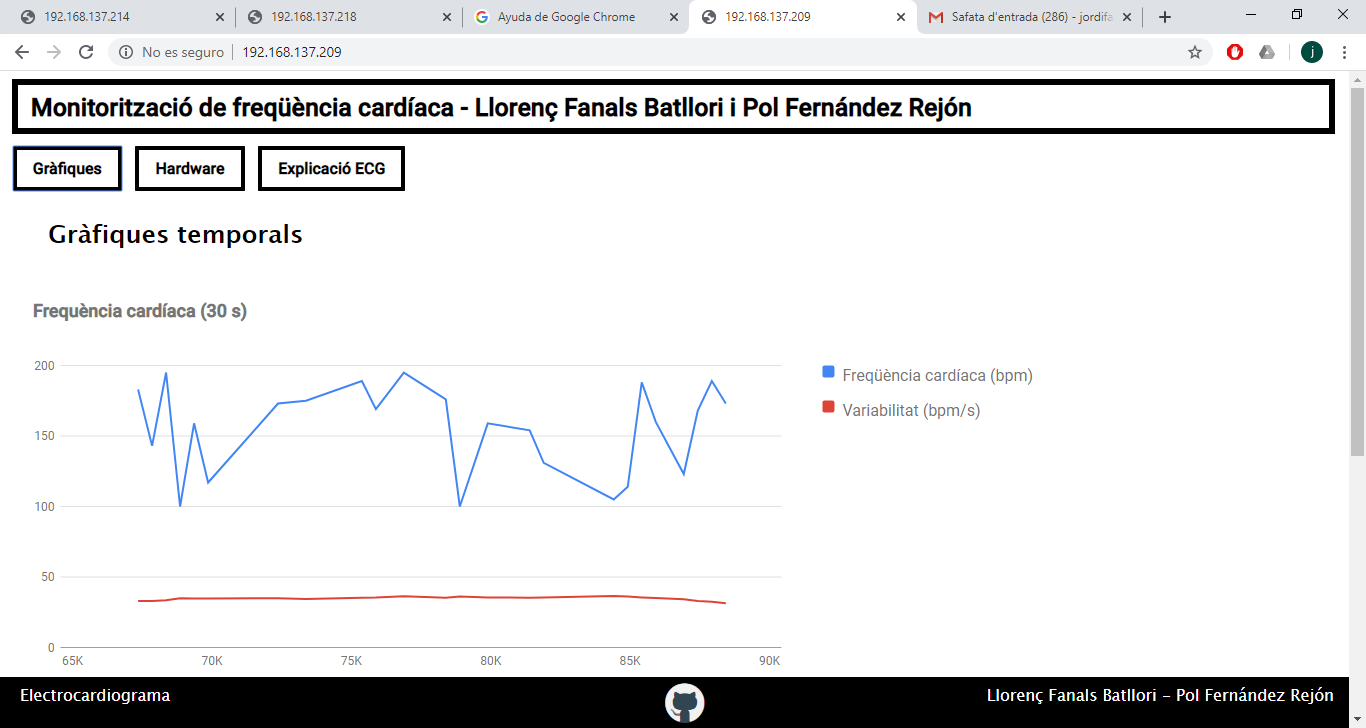
\includegraphics[scale=0.43]{images/web_ecg.png}}
\end{center}
\caption{Gràfica de les dades més recents, web}
\label{fig:1}
\end{figure}

\noindent \\ El fet d'utilitzar JavaScript permet inserir contingut dinàmic. Al passar el ratolí per sobre una línia es ressalta la línia i els punts que la formen. És possible visualitzar el valor de cada punt col·locant el ratolí sobre seu A la Figura \ref{fig:2} s'aprecia.
\begin{figure}[H]
\begin{center}
\fbox{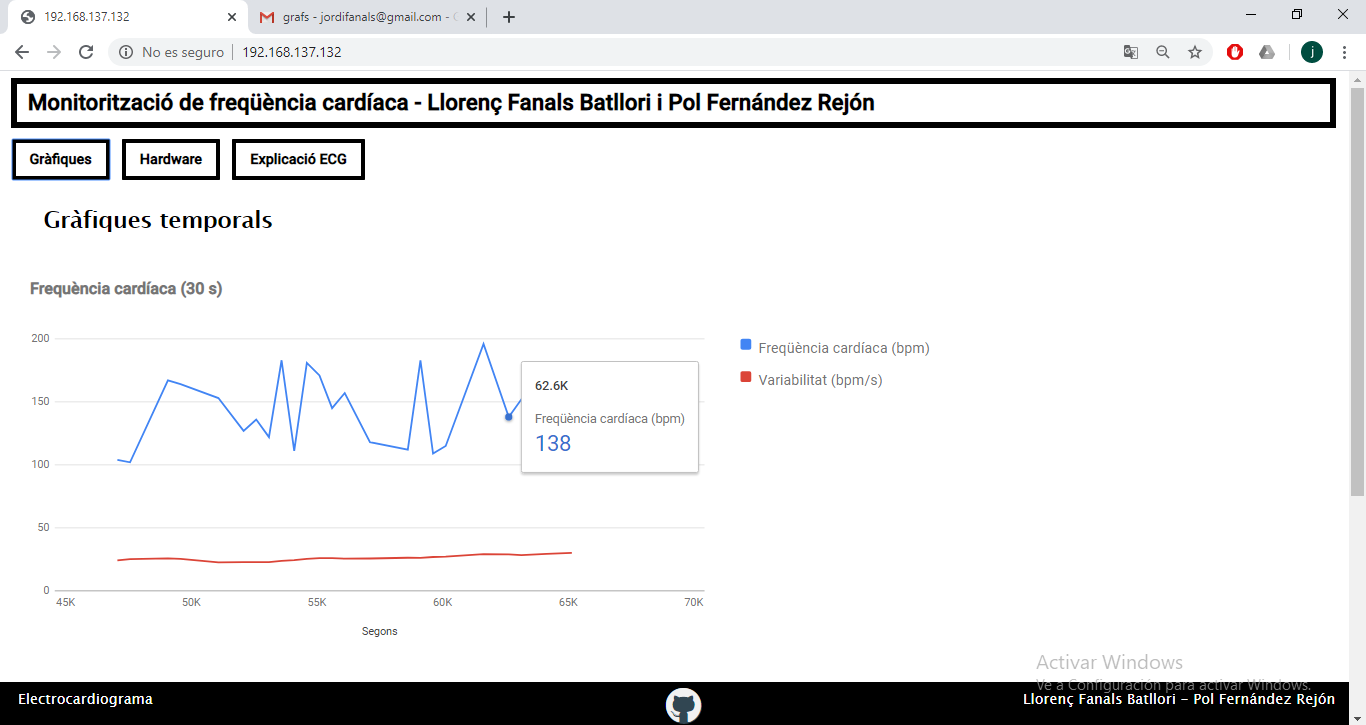
\includegraphics[scale=0.43]{images/web_punt.png}}
\end{center}
\caption{Gràfica ressaltant el valor d'un punt}
\label{fig:2}
\end{figure}

\noindent \\ Es pot navegar pels menús per veure un contingut o altre. Per exemple, podem demanar mirar l'apartat de hardware, i se'ns obra el següent:
\begin{figure}[H]
\begin{center}
\fbox{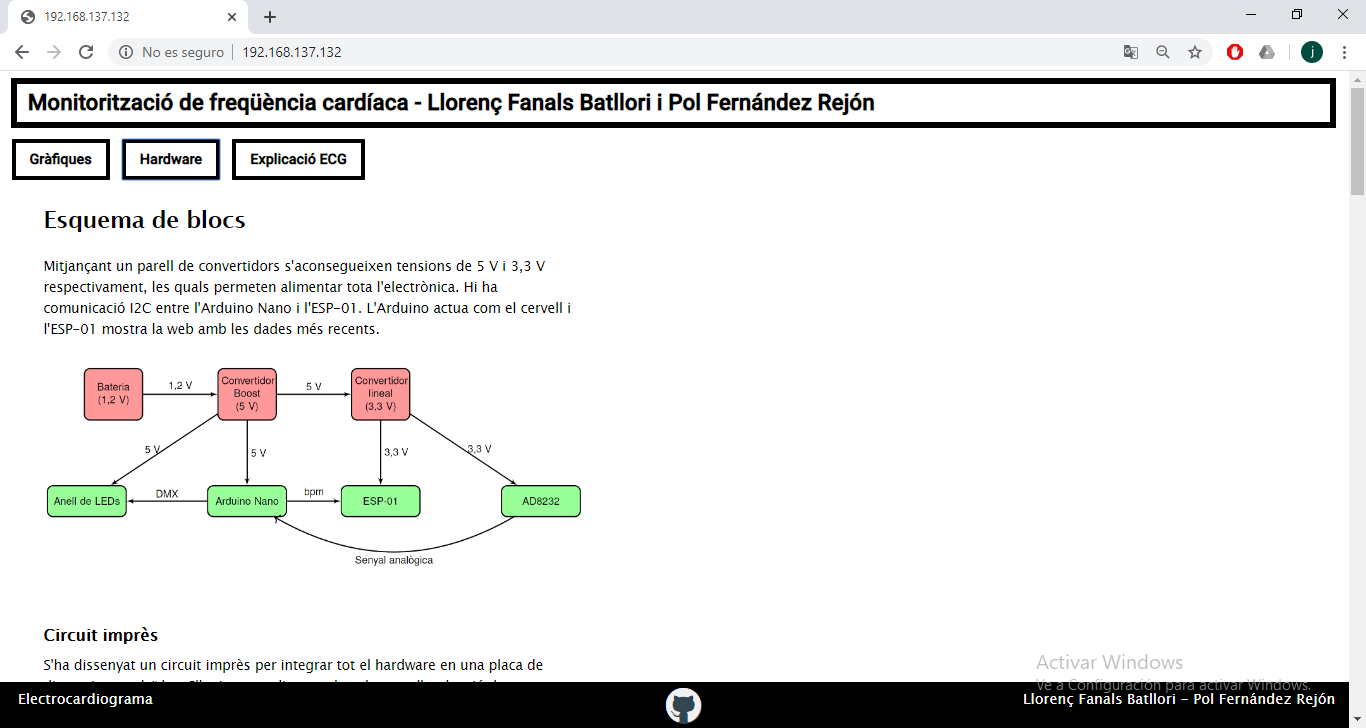
\includegraphics[scale=0.43]{images/web_hardware.png}}
\end{center}
\caption{Apartat de hardware}
\label{fig:2}
\end{figure}







\clearpage


% Table generated by Excel2LaTeX from sheet 'Hoja1'
%\begin{table}[H]
%  \centering
%    \begin{tabularx} {\textwidth} {|X|r|} \hline
%  \multicolumn{1}{|c|}{Descripció} &  \multicolumn{1}{c|}{Quantitat}\\ \hline \hline
%
 %   Placa GLC 330 W & 10 \\ \hline
%    Inversor FRONIUS Primo 3.0-1 Light 3kW & 1 \\ \hline
%    Metres cable Ethernet RJ-45 CAT 8 & 10 \\ \hline
%    Metres cable 4 m$m^2$ PVC & 45 \\ \hline
 %   Metres cable 1,5 m$m^2$ PVC & 100 \\ \hline
 %   Punteres Enghofer E 4-10, 4 m$m^2$, 10 mm & 20 \\ \hline
 %   Punteres Enghofer E 1.5-10 1,5 m$m^2$ 10 mm & 12 \\ \hline
 %   Cinta aïllant 10 m 1,6 cm & 3 \\ \hline
 %   Caixa estanca Solera CONS 100x100x55 mm & 2 \\ \hline
  %  Canal Euroquint 25,16 mm 1,5 metres & 20 \\ \hline
%    Curva canal VECAMCO & 10 \\ \hline
%    Paquet de 50 brides 200x2,6  mm & 2 \\ \hline
%    Regleta nylon 12 pols 16 mm & 4 \\ \hline
%    Premsaestopes M12 & 10 \\ \hline
%    Cargol autoroscant M4 16 mm & 12 \\ \hline
%    Tacs Fischer 072095 nylon 6x50 mm & 50 \\ \hline
%    Díode SM74611KTTR & 10 \\ \hline
%            Hores enginyer & 1 \\ \hline
%    Hores oficial de primera & 12 \\ \hline
%    Hores oficial de segona & 12 \\ \hline
%    \end{tabularx}%
%  \label{tab:addlabel}%
% \end{table}%

%\chapter{\uppercase{Instal·lació de l'electrònica}}
% Connexionat de les plaques electròniques amb la instal·lació elèctrica.



\clearpage


% Table generated by Excel2LaTeX from sheet 'Hoja1'
%\begin{table}[H]
%  \centering
%    \begin{tabularx} {\textwidth} {|X|r|} \hline
%  \multicolumn{1}{|c|}{Descripció} &  \multicolumn{1}{c|}{Quantitat}\\ \hline \hline
%
 %   Placa GLC 330 W & 10 \\ \hline
%    Inversor FRONIUS Primo 3.0-1 Light 3kW & 1 \\ \hline
%    Metres cable Ethernet RJ-45 CAT 8 & 10 \\ \hline
%    Metres cable 4 m$m^2$ PVC & 45 \\ \hline
 %   Metres cable 1,5 m$m^2$ PVC & 100 \\ \hline
 %   Punteres Enghofer E 4-10, 4 m$m^2$, 10 mm & 20 \\ \hline
 %   Punteres Enghofer E 1.5-10 1,5 m$m^2$ 10 mm & 12 \\ \hline
 %   Cinta aïllant 10 m 1,6 cm & 3 \\ \hline
 %   Caixa estanca Solera CONS 100x100x55 mm & 2 \\ \hline
  %  Canal Euroquint 25,16 mm 1,5 metres & 20 \\ \hline
%    Curva canal VECAMCO & 10 \\ \hline
%    Paquet de 50 brides 200x2,6  mm & 2 \\ \hline
%    Regleta nylon 12 pols 16 mm & 4 \\ \hline
%    Premsaestopes M12 & 10 \\ \hline
%    Cargol autoroscant M4 16 mm & 12 \\ \hline
%    Tacs Fischer 072095 nylon 6x50 mm & 50 \\ \hline
%    Díode SM74611KTTR & 10 \\ \hline
%            Hores enginyer & 1 \\ \hline
%    Hores oficial de primera & 12 \\ \hline
%    Hores oficial de segona & 12 \\ \hline
%    \end{tabularx}%
%  \label{tab:addlabel}%
% \end{table}%



%\chapter{\uppercase{Resum del pressupost}}
El pressupost inclou el pagament de la instal·lació dels panells, tota la instal·lació elèctrica, el muntatge de la placa i la programació. El pressupost és d'un total de set mil cinc-cents vint-i-dos euros amb setanta-un cèntims d'euro, sense IVA.


\clearpage
\chapter{\uppercase{Conclusió}}
Per desenvolupar el projecte s'han consultat fonts fiables en el camp de la medicina. Tot i ser una disciplina de la qual tenim idees molt vagues, hem entès com són les diferències de tensió que es poden captar en diferents llocs del cos humà. Un cop parlem de tensions, parlem d'electrònica, camp en què sí que tenim coneixements.\\
\newline El consum d'energia i les dimensions del hardware utilitzat han estat dues "constraints" que hem tingut en compte al llarg del desenvolupament. S'ha optat per una pila d'alta densitat energètica per tal d'optimitzar la relació energia/volum. Tot i utilitzar plaques de desenvolupament, s'ha aconseguit un volum de pocs centímetres cúbics, menor del de molts electrocardiògrafs comercials.\\
\newline La programació dels microcontroladors s'ha fet per tal de fer en paral·lel les tasques d'adquirir dades i la de mostrar-les al client. D'aquesta manera augmenta la robustesa del sistema. S'ha programat una web en HTML que inclou estils definits en CSS i contingut dinàmic en JavaScript. Considerem que té una interfície atractiva i intuïtiva.\\
\newline El client podrà conèixer amb precisió la freqüència cardíaca del pacient o persona que porti aquest aparell mitjançant una pàgina web. A la web apareixen les últimes dades de freqüència cardíaca així com les de l'últim dia. L'anell de LEDs és una forma molt visual de saber quina freqüència cardíaca té la persona.\\
\newline Els autors considerem que s'han complert satisfactòriament els objectius marcats a l'inici del projecte.

\vspace*{\fill}
\noindent Llorenç Fanals Batllori\\
Pol Fernández Rejón\\
Graduats en Enginyeria Electrònica Industrial i Automàtica\\
\\
\\
Girona, 14 de gener de 2020.

\clearpage
%\chapter{\uppercase{Relació de documents}}
El projecte està format per cinc documents, que són Memòria, Plànols, Plec de condicions, Estat d'amidaments i Pressupost.

\clearpage
\chapter{\uppercase{Bibliografia}}
GOOGLE. Line Chart by Google Charts. (https://developers.google.com/chart/interactive/docs/
gallery/linechart?hl=es, 20 de novembre de 2019) \\ \\
RANDOM NERD TUTORIALS. Build an ESP8266 Web Server - Code and Schematics. (https://randomnerdtutorials.com/esp8266-web-server/, 27 d'octubre de 2019) \\ \\
SUÁREZ, A., et al. Manual AMIR ECG. Academia MIR. 2010. \\ \\
VOWSTAR. NodeMCU Development Kit. (https://github.com/nodemcu/nodemcu-devkit-v1.0/blob/master/NODEMCU\_DEVKIT\_V1.0.PDF, 23 d'octubre de 2019)



%\clearpage
\chapter{\uppercase{Glossari}}
% ordenar alfebèticament
API: Application Programming Interface. \\ \\
CSS: Cascading Style Sheets
DC: Corrent Continu. \\ \\
ECG: Electrocardiogram \\ \\
HTML: HyperText Markyp Language. \\ \\
I2C: Inter-Integrated Circuit
RF: Radiofreqüència. \\ \\
SMD: Sourface Mount Device. \\ \\
SSID: Service Set Identifier. \\ \\
WIFI: Wireless Fidelity \\ \\



% PVC, AC, DC, USB, QGPC, REBT, 

\clearpage


\appendix

%\chapter{\uppercase{Càlculs}}
%\section{Càlculs línies elèctriques}
Per tal de calcular les seccions mínimes de les línies es té en compte la caiguda de tensió i la intensitat màxima admissible dels cables. El REBT indica a la ITC-BT-40 que els cables de connexió hauran d'estar dimensionats per una intensitat no inferior al 125\% de la intensitat màxima del generador. A més, la caiguda de tensió màxima permesa entre el generador i el punt d'interconnexió amb la xarxa és de 1,5\% respecte la tensió nominal.\\
\newline Recordar que les línies de connexió entre els panells solars, amb l'inversor i a la placa electrònica es té una senyal elèctrica de tipus continu. La línia que connecta la sortida de l'inversor amb la instal·lació interior és de senyal alterna, i es considera que amb un factor de potència unitari. El fabricant indica que el factor de potència de l'inversor escollit és sempre molt proper a la unitat.\\
\newline Per calcular la intensitat de les línies monofàsiques es fa servir l'Equació \ref{eq:il}:
\begin{equation} \label{eq:il}
I_{linia} = \frac{P}{V*\cos(\phi)}
\end{equation}
V = 230 V.\\
P: potència que consumeixen els elements connectats a la línia (W).\\
$\phi$: factor de potència.\\
\newline En monofàsic cal fer servir l'Equació \ref{eq:e}:
\begin{equation}\label{eq:e}
e(\%)=\frac{P}{V}\frac{2*l}{k*S}
\end{equation}
l: longitud ja sigui de la fase o el neutre des del comptador a l'element més llunyà (m).\\
$k = 56 m/mm^{2}\si{\ohm}$.\\
S:secció del cable (m$m^2$).\\
%
\newline El dimensionament de les línies ha de permetre que les caigudes de tensió no superin els màxims indicats prèviament. Alhora, els cables han de poder admetre les intensitats calculades, per això ens guiem amb la taula de la ITC-19 del REBT. Finalment, cal comprovar que  l'interruptor magnetotèrmic té una intensitat nominal superior a la calculada per la línia i menor a l'admissible que marca la ITC-19.\\
\newline S'ha de tenir en compte el factor de correcció per radiació directa del Sol ($F_{sol}$), tal i com es comenta a la ITC-BT-06. S'escull un factor per radiació directa del Sol de 0,9.\\
\newline També s'ha de tenir en compte el factor de correcció per agrupament de cables ($F_{grup}$) de 0,89 per parelles de cables i de 0,75 per l'agrupament de cables que va a la placa electrònica, tal com marca la ITC-BT-06 que tracta sobre instal·lacions aèries.\\
\newline Finalment, el tercer factor és el factor de correcció per temperatura ($F_{temp}$), que s'escull de 0,9, que és el factor que s'ha d'agafar segons la ITC-BT-06 per temperatures de 50 $^\circ$C.\\
%
%
%
%
\newline Per totes les línies menys per la de connexionat la placa electrònica es té en compte un factor de 1,25, tal com marca la ITC-BT-19 per generadors. La caiguda de tensió no pot ser major de l'1,5\% respecte la tensió nominal.\\
\newline Es decideix instal·lar cables de recobriment de PVC sobre paret, muntatge C6.\\
%
\newline Amb aquests factors coneguts es pot calcular la intensitat de càlcul de les diferents línies, a partir de la qual es determinen les seccions.\\
\newline La intensitat de curtcircuit augmenta amb la temperatura un 0,055\% per grau centígrad. Es calcula a 70 C$^{\circ}$ la intensitat de curtcircuit en condicions de 1.000 W/$m^2$. La que facilita el fabricant és de 9,33 A a 25 C$^{\circ}$.\\
\newline Per conèixer la intensitat màxima de curtcircuit, en el cas més desfavorable, cal seguir l'Equació \ref{eq:isc}:
\begin{equation} \label{eq:isc}
I_{sc}(T=70\  C ^{\circ})= I_{sc} (1 + \alpha (T-25 \ C^{\circ}))
\end{equation}

\noindent $I_{sc}$: intensitat de curtcircuit del panell a 25 C$^{\circ}$ (A).\\
$\alpha$: factor lineal d'increment d'intensitat de curtcircuit per efecte de la temperatura (\%).\\
T: temperatura, en aquest cas 70 C$^{\circ}$.\\
\noindent El resultat és de 9,56 A.\\
%
\newline Per calcular la tensió màxima de circuit obert s'ha fet servir l'Equació \ref{eq:isc}:
\begin{equation} \label{eq:isc}
V_{oc}(T=-10\  C ^{\circ})= V_{oc} (1 + \beta (T-25 \ C^{\circ}))
\end{equation}
\noindent  $V_{oc}$: Tensió de circuit obert a 25 C$^{\circ}$ (V).\\
$\beta$: factor lineal de decrement de tensió de circuit obert per efecte de la temperatura (\%).\\
%
\newline La tensió de circuit obert a 25 C$^{\circ}$ és de 46,2 V. El factor lineal que indica el fabricant és de -0,32\%/C$^{\circ}$, que dona un total de 51,37 V. S'han tingut en compte pel dimensionament de la placa electrònica.\\
\newline Dit això, per calcular les seccions dels cables cal destacar que el producte de la intensitat de curtcircuit calculada per la temperatura més desfavorable multiplicada per 1,25 ha de ser igual a la secció del REBT multiplicada pels factors de radiació solar, agrupament i temperatura.\\
\newline Si s'aïlla, es pot dir que la intensitat de curtcircuit calculada multiplicada per 1,25 i dividida pels factors mencionats ha de ser admesa per les seccions dels cables del REBT.\\
\newline A la Taula \ref{tab:taulax} es detalla la intensitat de cada línia i els factors que cal tenir en compte.

\begin{table}[H]
\scriptsize
  \centering
    \begin{tabu} to \textwidth  {|X[0.3, l]|X[2, l]|X[0.5, r]|X[0.6, r]|X[0.5, r]|X[0.5, r]|X[0.5, r]|} \hline
Línia &  Descripció & Intensitat (A) & Factor generador & Factor radiació solar & Factor agrupament  & Factor temperatura\\ \hline \hline
L1 & Connexionat entre els panells solars & 9,56 & 1,25 & 0,9 & 0,89 & 0,9 \\ \hline
L2 & Connexionat de la branca 1 a l'inversor & 9,56 & 1,25 & 0,9 & 0,89 & 0,9\\ \hline
L3 & Connexionat de la branca 2 a l'inversor & 9,56 & 1,25 & 0,9 & 0,89 & 0,9\\ \hline
L4 & Connexionat de l'inversor al QGPC & 14,3 & 1,25 & 1,0 & 1,00 & 1,0 \\ \hline \hline
L5 & Línies de connexionat dels panells fotovoltaics a la placa electrònica & 0,0023 & 1,00 & 0,9 & 0,75 & 0,9 \\ \hline
	
    \end{tabu}%
  \caption{Intensitat de càlcul pel dimensionament de les línies}
    \label{tab:taulax}%
 \end{table}%

\noindent Amb aquesta intensitat de càlcul podem dimensionar les línies. Es calculen les seccions per tal d'evitar tenir un percentatge de caiguda de tensió entre els generadors i el punt de connexió a la xarxa superior de 1,5\%, tal com marca la ITC-BT-40 de generadors.\\
\newline A la Taula \ref{tab:t2} es mostren dades de les diverses línies detallades.\\
\newline L'inversor sempre intenta donar els 230 V a la seva sortida, sempre que el valor de l'entrada superi els 80 V mínims que marca el fabricant. S'ha acumulat la caiguda de tensió de la línia 1 amb la línia 2 i la 3; i la més desfavorable entre la 2 i la 3 amb la 4. La ITC-BT-19 verifica que per intensitats admissibles les seccions són correctes.
%
\begin{table}[H]
\scriptsize
\begin{center}
 \begin{tabu} to 0.985\textwidth {|X[0.5, l]|X[1.5, l]|X[0.8, r]|X[0.6, r]|X[r]|X[r]|X[r]|X[r]|X[r]|X[r]|X[0.5,r]|}%{X | c c c} 
 \hline
 Línia& Descripció & Potència (W) & cos($\phi$) & Intensitat nominal (A) & Distància màxima (m) & Seccions ($mm^{2}$) & Diàmetre tub (mm) & Caiguda de tensió (\%) & Caiguda de tensió acum. (\%)\\
 \hline \hline 

L1 & Connexionat entre els panells solars & 1.650 & 1 & 9,56 & 10 & 2x4 & 20 & 0,42 & 0,42 \\ \hline
L2 & Connexionat de la branca 1 a l'inversor & 1.650  & 1 & 9,56  & 30 & 2x10 & 20 & 0,50 & 0,92 \\ \hline 
L3 & Connexionat de la branca 2 a l'inversor & 1.650  & 1 & 9,56  & 19 & 2x6 & 25 & 0,53 & 0,95 \\ \hline 
L4 & Connexionat de l'inversor al QGPC & 3.300  & 1 & 14,35 & 6 & 2x4 + 4 & 25 & 0,38 & 1,33 \\ \hline \hline
L5 & Línies de connexionat dels panells fotovoltaics a la placa electrònica & 0,529 & 1 & 0,0038& 21 & 2x1,5 & 32 & 0,000575 & 0,000575 \\ \hline 


 \end{tabu}
 \caption{Línies detallades}
 \label{tab:t2}%
\end{center}
\end{table}

 
 
%
%




%\section{Càlculs placa electrònica}
% o hauria de dir instrumentació?



\clearpage


% Table generated by Excel2LaTeX from sheet 'Hoja1'
%\begin{table}[H]
%  \centering
%    \begin{tabularx} {\textwidth} {|X|r|} \hline
%  \multicolumn{1}{|c|}{Descripció} &  \multicolumn{1}{c|}{Quantitat}\\ \hline \hline
%
 %   Placa GLC 330 W & 10 \\ \hline
%    Inversor FRONIUS Primo 3.0-1 Light 3kW & 1 \\ \hline
%    Metres cable Ethernet RJ-45 CAT 8 & 10 \\ \hline
%    Metres cable 4 m$m^2$ PVC & 45 \\ \hline
 %   Metres cable 1,5 m$m^2$ PVC & 100 \\ \hline
 %   Punteres Enghofer E 4-10, 4 m$m^2$, 10 mm & 20 \\ \hline
 %   Punteres Enghofer E 1.5-10 1,5 m$m^2$ 10 mm & 12 \\ \hline
 %   Cinta aïllant 10 m 1,6 cm & 3 \\ \hline
 %   Caixa estanca Solera CONS 100x100x55 mm & 2 \\ \hline
  %  Canal Euroquint 25,16 mm 1,5 metres & 20 \\ \hline
%    Curva canal VECAMCO & 10 \\ \hline
%    Paquet de 50 brides 200x2,6  mm & 2 \\ \hline
%    Regleta nylon 12 pols 16 mm & 4 \\ \hline
%    Premsaestopes M12 & 10 \\ \hline
%    Cargol autoroscant M4 16 mm & 12 \\ \hline
%    Tacs Fischer 072095 nylon 6x50 mm & 50 \\ \hline
%    Díode SM74611KTTR & 10 \\ \hline
%            Hores enginyer & 1 \\ \hline
%    Hores oficial de primera & 12 \\ \hline
%    Hores oficial de segona & 12 \\ \hline
%    \end{tabularx}%
%  \label{tab:addlabel}%
% \end{table}%


\end{spacing}
\begin{spacing}{1}

\chapter{\uppercase{Programes}}

\section{Programa Arduino Nano}
\begin{lstlisting}[style=myArduino]
/* Llorenç Fanals Batllori
 * Pol Fernández Rejón
 * Electrocardiógraf amb connectivitat WiFi
 * Codi Arduino Nano
 */
 
#include <Wire.h> // Per comunicar per I2C
int randNumber;   // Nombre aleatori que es generava per testejar
char cadena[3];   // Guarda la frequència cardíaca

#include <Adafruit_NeoPixel.h> // Llibreria per controlar l'anell de LEDs
#ifdef __AVR__
#include <avr/power.h>
#endif
#define LED_PIN    6           // S'utilitza el pin digital número 6
#define LED_COUNT 16           // Anell de 16 LEDs

Adafruit_NeoPixel strip(LED_COUNT, LED_PIN, NEO_GRB + NEO_KHZ800);

uint32_t off = strip.Color(0, 0, 0);
long int temps_memoria = 0;
long int temps_memoria_2 = 0;
int i = 0;
const int delay_entre_leds = 20;
const int delay_refresc = 1000;
int32_t c0 = strip.Color(255, 255, 0);
uint32_t c1 = strip.Color(178, 255, 0);
uint32_t c2 = strip.Color(55, 255, 0);
uint32_t c3 = strip.Color(6, 172, 38);
uint32_t c4 = strip.Color(0, 210, 255);
uint32_t c5 = strip.Color(8, 0, 255);
uint32_t c6 = strip.Color(1, 0, 255);
uint32_t c7 = strip.Color(107, 0, 222);
uint32_t c8 = strip.Color(101, 0, 144);
uint32_t c9 = strip.Color(255, 0, 208);
uint32_t c10 = strip.Color(255, 0, 199);
uint32_t c11 = strip.Color(123, 0, 96);
uint32_t c12 = strip.Color(128, 0, 46);
uint32_t c13 = strip.Color(223, 2, 10);
uint32_t c14 = strip.Color(223, 0, 0);
uint32_t c15 = strip.Color(255, 0, 0);
uint32_t leds[16]={c0, c1, c2, c3, c4, c5, c6, c7, c8, c9, c10, c11, c12, c13, c14, c15};
long int freq_bpm;

long int temps_pic_anterior = 0;
int llindar_max = 600;
int llindar_min = 500;
int lectura_analogica = 0;
int diferencia_temps = 0;
bool pic = 0;

bool dada_enviada = 0;

void setup() {
  Wire.begin(8);  //0x08=8, adreça que fem servir per comunicar amb l'ESP-01
//  Wire.onReceive(receiveEvent);
  Wire.onRequest(sendEvent);
  Serial.begin(9600);  // Habilitem el port sèrie, va bé per visualitzar l'electrocardiograma

  randomSeed(analogRead(1)); // Per generar nombres random

// ----------------------------

  #if defined(__AVR_ATtiny85__) && (F_CPU == 16000000)
    clock_prescale_set(clock_div_1);
  #endif
  
    strip.begin();           // Inizialitza l'anell
    strip.show();            // Apaga tots els LEDs
    strip.setBrightness(70); // Estableix la lluminositat, el màxim és 255, PWM

    // Illuminem cada LED amb el seu color
    strip.setPixelColor(0, c0);
    strip.setPixelColor(1, c1);
    strip.setPixelColor(2, c2);
    strip.setPixelColor(3, c3);
    strip.setPixelColor(4, c4);
    strip.setPixelColor(5, c5);
    strip.setPixelColor(6, c6);
    strip.setPixelColor(7, c7);
    strip.setPixelColor(8, c8);
    strip.setPixelColor(9, c9);
    strip.setPixelColor(10, c10);
    strip.setPixelColor(11, c11);
    strip.setPixelColor(12, c12);
    strip.setPixelColor(13, c13);
    strip.setPixelColor(14, c14);
    strip.setPixelColor(15, c15);
      
    strip.show(); // Indiquem que volem aplicar els canvis generats

    temps_memoria_2 = millis();
    
    temps_pic_anterior = millis();
}

void loop() {
 // sendEvent(2);
 
    lectura_analogica = analogRead(A0);
    Serial.println(analogRead(A0));
    
 // Analitzem si s'ha donat un pic
    if (lectura_analogica>llindar_max && pic == 0)
    {
      diferencia_temps = millis() - temps_pic_anterior;
      temps_pic_anterior = millis();
      pic = 1;
      freq_bpm = (60.0*1000.0 / diferencia_temps);
      dada_enviada = 0;
      i=0;
      strip.fill(off, 0, 16);
      strip.show();
    }
    else if (lectura_analogica < llindar_min && pic==1){
      pic = 0;
    }

  // Determinem si cal encendre leds o no
    if ((millis()-temps_memoria_2) > delay_entre_leds)
    {
      if (i<freq_bpm*16/130)
      {
       strip.setPixelColor(i, leds[i]);
       strip.show();
      i++;      
      }
      temps_memoria_2 = millis();
    }

}

// TODO: enviar la frequencia enlloc d'un numero random, i com a condicional tenir un boolea que digui si cal enviar o no
void sendEvent(int howmany){
  // Funció per respondre per I2C a l'ESP-01
  /*
  randNumber = random(40, 200); // Serial.print("generat: "); Serial.println(randNumber);
  
  cadena[2] = (randNumber - (randNumber/10)*10) + 48; 
  cadena[1] = (randNumber/10 - (randNumber/100)*10) + 48; 
  cadena[0] = (randNumber / 100) + 48; 
  // Serial.println(cadena);

  if (randNumber >= 40){
    Wire.write(cadena); // Serial.println("major de 100");
  }
 //  Wire.endTransmission(true);
 // Wire.write(cadena); // 3 bytes
 */
  
  cadena[2] = (freq_bpm - (freq_bpm/10)*10) + 48; 
  cadena[1] = (freq_bpm/10 - (freq_bpm/100)*10) + 48; 
  cadena[0] = (freq_bpm / 100) + 48; 
  if (dada_enviada == 0){
    Wire.write(cadena);
    dada_enviada = 1;
  }

}


/*
void receiveEvent(int howMany){
  String recibido;
  while (0 < Wire.available()) {
    char c = Wire.read();
    recibido += c;
  }
  Serial.print(recibido);
}
*/

\end{lstlisting}

\section{Programa ESP-01}

\begin{lstlisting}[style=myArduino]
/*********
  Llorenç Fanals Batllori
  Pol Fernández Rejón
  Graduat en Enginyeria Electrònica Industrial i Automàtica
  20/11/2019
*********/
#include <Wire.h>
String recibido;

int i_fila = 0;
int i_columna = 0;

#include <ESP8266WiFi.h> // Es carrega la llibreria Wi-Fi

// Credencials de la xarxa Wi-Fi a què ens volem connectar
// const char* ssid     = "DESKTOP-E5M4HBA 4049";
// const char* password = "E^1w1736";

const char* ssid     = "DESKTOP-MQE758J 3309";
const char* password = "04)R936v";

// Port que volem utilitzar. El 80 és el port per defecte, així que teclejant la IP a un navegador en farem prou. Si fos un altre port la IP acabaria en ":número_port".
WiFiServer server(80);


unsigned long TempsActual = millis(); // Current time
unsigned long TempsAnterior = 0; // Previous time
const long TempsConnectat = 100; // Define timeout time in milliseconds (example: 2000ms = 2s)


#define files 24
#define columnes 5

float vector[files][columnes]; // vector de dades
float vector2[files][columnes]; // vector de dades
int i = 0; // iterador per files
int j = 0; // iterador per columnes

#define D0 16
#define D1 5
#define D2 4
#define D3 0

#define ENTRADA_ANALOGICA A0

unsigned int hores_posada_marxa = 10; // l'hora en què es fa la posada en marxa
unsigned int minuts_posada_marxa = 23; // a les 10:23 es fa la posada en marxa

unsigned int hora_actual;
float minuts_actual;
unsigned int millis_anteriors;

void inicialitza_vectors() { // Emplena els vectors de dades fictícies. A còpia d'hores s'aniran reemplaçant per dades reals
  //temps, bpm, pendent bpm
  vector[0][0] = 0; vector[0][1] = 0; vector[0][2] = 0;
  vector[1][0] = 0; vector[1][1] = 0; vector[1][2] = 0;
  vector[2][0] = 0; vector[2][1] = 0; vector[2][2] = 0;
  vector[3][0] = 0; vector[3][1] = 0; vector[3][2] = 0;
  vector[4][0] = 0; vector[4][1] = 0; vector[4][2] = 0;
  vector[5][0] = 0; vector[5][1] = 0; vector[5][2] = 0;
  vector[6][0] = 0; vector[6][1] = 0; vector[6][2] = 0;
  vector[7][0] = 0; vector[7][1] = 0; vector[7][2] = 0;
  vector[8][0] = 0; vector[8][1] = 0; vector[8][2] = 0;
  vector[9][0] = 0; vector[9][1] = 0; vector[9][2] = 0;
  vector[10][0] = 0; vector[10][1] = 0; vector[10][2] = 0;
  vector[11][0] = 0; vector[11][1] = 0; vector[11][2] = 0;
  vector[12][0] = 0; vector[12][1] = 0; vector[12][2] = 0;
  vector[13][0] = 0; vector[13][1] = 0; vector[13][2] = 0;
  vector[14][0] = 0; vector[14][1] = 0; vector[14][2] = 0;
  vector[15][0] = 0; vector[15][1] = 0; vector[15][2] = 0;
  vector[16][0] = 0; vector[16][1] = 0; vector[16][2] = 0;
  vector[17][0] = 0; vector[17][1] = 0; vector[17][2] = 0;
  vector[18][0] = 0; vector[18][1] = 0; vector[18][2] = 0;
  vector[19][0] = 0; vector[19][1] = 0; vector[19][2] = 0;
  vector[20][0] = 0; vector[20][1] = 0; vector[20][2] = 0;
  vector[21][0] = 0; vector[21][1] = 0; vector[21][2] = 0;
  vector[22][0] = 0; vector[22][1] = 0; vector[22][2] = 0;
  vector[23][0] = 0; vector[23][1] = 0; vector[23][2] = 0;

  vector2[0][0] = 0; vector2[0][1] = 0; vector2[0][2] = 0;
  vector2[1][0] = 1; vector2[1][1] = 0; vector2[1][2] = 0;
  vector2[2][0] = 2; vector2[2][1] = 0; vector2[2][2] = 0;
  vector2[3][0] = 3; vector2[3][1] = 0; vector2[3][2] = 0;
  vector2[4][0] = 4; vector2[4][1] = 0; vector2[4][2] = 0;
  vector2[5][0] = 5; vector2[5][1] = 0; vector2[5][2] = 0;
  vector2[6][0] = 6; vector2[6][1] = 0; vector2[6][2] = 0;
  vector2[7][0] = 7; vector2[7][1] = 0; vector2[7][2] = 0;
  vector2[8][0] = 8; vector2[8][1] = 0; vector2[8][2] = 0;
  vector2[9][0] = 9; vector2[9][1] = 0; vector2[9][2] = 0;
  vector2[10][0] = 10; vector2[10][1] = 0; vector2[10][2] = 0;
  vector2[11][0] = 11; vector2[11][1] = 0; vector2[11][2] = 0;
  vector2[12][0] = 12; vector2[12][1] = 0; vector2[12][2] = 0;
  vector2[13][0] = 13; vector2[13][1] = 0; vector2[13][2] = 0;
  vector2[14][0] = 14; vector2[14][1] = 0; vector2[14][2] = 0;
  vector2[15][0] = 15; vector2[15][1] = 0; vector2[15][2] = 0;
  vector2[16][0] = 16; vector2[16][1] = 0; vector2[16][2] = 0;
  vector2[17][0] = 17; vector2[17][1] = 0; vector2[17][2] = 0;
  vector2[18][0] = 18; vector2[18][1] = 0; vector2[18][2] = 0;
  vector2[19][0] = 19; vector2[19][1] = 0; vector2[19][2] = 0;
  vector2[20][0] = 20; vector2[20][1] = 0; vector2[20][2] = 0;
  vector2[21][0] = 21; vector2[21][1] = 0; vector2[21][2] = 0;
  vector2[22][0] = 22; vector2[22][1] = 0; vector2[22][2] = 0;
  vector2[23][0] = 23; vector2[23][1] = 0; vector2[23][2] = 0;
}

int n_rebut = 0;
float mitjana = 0;
float desvest = 0;
int n_dades_hora = 0;
float sumatori_2 = 0;

void setup() {
  Wire.begin(0, 2); // nodemcu: 4,5; esp-01: 0,2

  hora_actual = 0; // hores_posada_marxa
  minuts_actual = 0; // minuts_posada_marxa

  // Dades temporals dels vectors. Serveixen per mostrar com queden representades les gràfiques. S'aniran borrant les dades més antigues.
  inicialitza_vectors();

  Serial.begin(115200); // Habilitem el port sèrie a 115200 de baud rate

  // Ens connectem al Wi-Fi amb l'adreça i la contrasenya definits
  Serial.print("Connectant a: ");
  Serial.println(ssid); // Mostrem l'adreça del Wi-Fi
  WiFi.begin(ssid, password); // Iniciem la comunicació

  while (WiFi.status() != WL_CONNECTED) {
    delay(500);
    Serial.print("."); // Cada 0,5 s que passin sense connectar-se mostra un punt
  }

  // S'ha connectat
  Serial.println("");
  Serial.println("WiFi connectat");
  Serial.println("Adreça IP: ");
  Serial.println(WiFi.localIP());
  server.begin();

}

void demana_dada (){
  Wire.requestFrom(8, 3); //0x08 = 8;

  while (0 < Wire.available()) {
    char c = Wire.read(); 
    int nombre = c-48; 
    //  Serial.println(nombre);
    n_rebut = n_rebut*10 + (c-48);
  }

  if (n_rebut != -2523 && n_rebut != 0){
  
      vector[i_fila][0] = millis()/1000.0;
      vector[i_fila][1] = n_rebut;
      
          for (i=0; i<files; i++){
            mitjana = vector[i][1]*(1.0/(i+1.0)) + mitjana*i/(i+1.0);  
          }
          int sumatori = 0;
          for (i=0; i<files; i++){
            sumatori += (mitjana - vector[i][1]) * (mitjana - vector[i][1]);  
          }
          desvest = sumatori / (files-1);
  
      vector[i_fila][2] = 1.0*pow(desvest, 0.5);
    // 2 ms per fer els càlculs de mitjana i desvest, acceptable  
          
      i_fila++;
      if (i_fila > files) {
        i_fila = 0;
      }
   
      Serial.println(n_rebut);  
  
  //----- dades hora, 2a gràfica -----
  
      n_dades_hora++;
      vector2[hora_actual][0] = hora_actual;
      vector2[hora_actual][1] = n_rebut*1.0/(n_dades_hora) + vector[hora_actual][1]*(n_dades_hora-1)/(n_dades_hora);
      vector2[hora_actual][2] = vector[i_fila-1][2]*1.0/(n_dades_hora) + vector2[hora_actual][2]*(n_dades_hora-1)/(n_dades_hora);
  }
    
  else {
      Serial.println("és -2523"); // l'Arduino Nano no té cap dada nova, captem aquest número
  }

    n_rebut = 0;
    Wire.endTransmission(); // Afegit, no fa cap mal
}

void loop() {
  //  Wire.beginTransmission(8);//0x08 = 8;
  //  Wire.write("esp to uno \n");
  //  Wire.endTransmission();
  // int temps_xyz = millis();
  
  demana_dada();
  delay(50); // 100

// ---------------------------------------------------------------------------------------------

  WiFiClient client = server.available();   // Escolta si hi ha clients

  if (client) {                             // Si es connecta un nou client,
    Serial.println("Nou client.");
    String LiniaActual = "";                // una cadena memoritza la informació enviada pel client
    TempsActual = millis();
    TempsAnterior = TempsActual;
    while (client.connected() && TempsActual - TempsAnterior <= TempsConnectat) { // Si estem connectats i no han passat els milisegons que indica TempsConnectat,

      TempsActual = millis();
      if (client.available()) {             // Si el client ens passa informació,
        char c = client.read();             // llegim un caràcters ascii (un byte)
        Serial.write(c);                    // i el mostrem per pantalla
        if (c == '\n') {                    // Si rebem un canvi de línia com a caràcter,
          // és el final de la petició HTTP
          if (LiniaActual.length() == 0) {
            // Ara responem donant un OK i indicant el content type, volem una pàgina html. Finalment una línia en blanc, és el protocol
            client.println("HTTP/1.1 200 OK");
            client.println("Content-type:text/html");
            client.println("Tancant connexió");
            client.println();
            client.println("<!DOCTYPE html><html>");
            client.println("<head><meta name=\"viewport\" content=\"width=device-width, initial-scale=1\">");
            client.println("    <meta charset=\"UTF-8\">\n<meta http-equiv=\"Content-type\" content=\"text/html; charset=UTF-8\">");
            client.println("<link rel=\"icon\" href=\"data:,\">");
            client.println("    <link rel=\"stylesheet\" href=\"https://use.fontawesome.com/releases/v5.7.2/css/all.css\" integrity=\"sha384-fnmOCqbTlWIlj8LyTjo7mOUStjsKC4pOpQbqyi7RrhN7udi
            9RwhKkMHpvLbHG9Sr\" crossorigin=\"anonymous\">\n""");
            client.println("    <script type=\"text/javascript\" src=\"https://www.gstatic.com/charts/loader.js\"></script>\n    <script type=\"text/javascript\">\n      google.charts.load('current', {'packages':['line']});\n      google.charts.setOnLoadCallback(drawChart);\n\n");
            
            // Definim la gràfica de la primera branca
            client.println("    function drawChart() {\n\n      var data = new google.visualization.DataTable();\n      data.addColumn('number', 'Segons');\n      data.addColumn('number', 'Frequència cardíaca (bpm)');\n      data.addColumn('number', 'Variabilitat (bpm/s)');");

            client.println("\n data.addRows([\n");
            for (i = i_fila; i < files; i++) {
              client.println("[");
              client.println(String(vector[i][0]));
              for (j = 1; j < 3; j++) {
                client.println(","); client.println(String(vector[i][j]));
              }
              client.println("]"); client.println(","); client.println("\n");
            }

            for (i = 0; i < i_fila; i++) {
              client.println("[");
              client.println(String(vector[i][0]));
              for (j = 1; j < 3; j++) {
                client.println(","); client.println(String(vector[i][j]));
              }
              client.println("]"); client.println(","); client.println("\n");
            }
            
          client.println("]);\n\n\n  var options = {\n            'width': 1000,\n            'height': 400,\n        chart: {\n          title: 'Frequència cardíaca (30 s)',\n          bold: true, \n          // subtitle: 'in millions of dollars (USD)'\n          width: 100,\n        },\n        titleTextStyle: {\n          bold: true,\n          fontSize: 18,\n        }\n     //   width: 900,\n     //   height: 500\n      };\n\n      var chart = new google.charts.Line(document.getElementById('linechart_material'));\n\n      chart.draw(data, google.charts.Line.convertOptions(options));\n    }\n    </script>");
          // Definim la gràfica de la segona branca
          client.println(" \n\n   <script type=\"text/javascript\" src=\"https://www.gstatic.com/charts/loader.js\"></script>\n    <script type=\"text/javascript\">\n    google.charts.load('current', {'packages':['line']});\n    google.charts.setOnLoadCallback(drawChart);\n    \n\n    function drawChart() {\n\n    var data = new google.visualization.DataTable();\n    data.addColumn('number', 'Hora');\n      data.addColumn('number', 'Freqüència cardíaca (bpm)');\n      data.addColumn('number', 'Variabilitat (bpm/s)');");
/*           
            client.println("data.addRows([\n"); 
            for (i = hora_actual+1; i < files; i++) { // i = hora_actual ...
              client.println("[");
              client.println(String(vector2[i][0]));
              for (j = 1; j < 3; j++) {
                client.println(","); client.println(String(vector2[i][j]));
              }
              client.println("]"); client.println(","); client.println("\n");
            }
*/
            client.println("data.addRows([\n"); 
            for (i = 0; i < files; i++) { // i = hora_actual ...
              client.println("[");
              client.println(String(vector2[i][0]));
              for (j = 1; j < 3; j++) {
                client.println(","); client.println(String(vector2[i][j]));
              }
              client.println("]"); client.println(","); client.println("\n");
            }
/*
            for (i = 0; i < hora_actual+1; i++) {
              client.println("[");
              client.println(String(vector2[i][0]));
              for (j = 1; j < 3; j++) {
                client.println(","); client.println(String(vector2[i][j]));
              }
              client.println("]"); client.println(","); client.println("\n");
            }
*/
    client.println(" ]); \n\n\n\n   var options = {\n      'width': 1000,\n      'height': 400,\n        chart: {\n        title: 'Freqüència cardíaca (1 dia)',\n       // is3D: true\n        // subtitle: 'in millions of dollars (USD)'\n        },\n      titleTextStyle: {\n        bold: true,\n        fontSize: 18,\n      }\n     //   width: 700,\n     //   height: 400\n    };\n\n    var chart = new google.charts.Line(document.getElementById('linechart_material2'));\n\n    chart.draw(data, google.charts.Line.convertOptions(options));\n    }\n    </script>\n\n  </head>\n\n  <style>\n        .content {\n          max-width: 100%;\n          margin: left;\n        }\n   </style>\n\n<!--  
    ###############################################
    #####################################   -->\n\n    <style>\nul {\n  list-style-type: none;\n  margin: 0;\n  padding: 0;\n  overflow: hidden;\n  background-color: #333;\n}\n\nli {\n  float: left;\n}\n\nli a {\n  display: block;\n  color: white;\n  text-align: center;\n  padding: 14px 16px;\n  text-decoration: none;\n}\n\n/* Change the link color to #111 (black) on hover */\nli a:hover {\n  background-color: #f3f3f3;\n}\n\n.active {\n    background-color: #4CAF50;\n  }\n\n  li {\n    border-right: 1px solid #bbb;\n  }\n  \n  li:last-child {\n    border-right: none;\n  }\n\n  ul {\n    position: fixed;\n    top: 0;\n    width: 100%;\n  }\n/*\n  div{\n    display: none;\n}*/\n    \n.button {\n    align-items: right;\n    font-size: 16px;\n    display:inline-block;\n    padding:0.55em 1.0em;\n    border:0.25em solid #000000;\n    margin:0.3em 0.3em 0.3em 0.3em;\n    border-radius:0.05em;\n    box-
    sizing: border-box;\n    text-decoration:none;\n    font-family:'Roboto',sans-serif;\n    font-weight:800;\n    color:#000000;\n    text-align:center;\n    transition: all 0.2s;\n\n    background-color: #ffffff;\n    }\n    .button:hover{\n    color:#ffffff;\n    background-color:#000000;\n    }\n    @media all and (max-width:30em){\n    .button{\n    display:block;\n    margin:0.4em auto;\n    }\n    }\n\n    p.solid {\n             font-size: 25px;\n             font-weight: bold;\n             margin:0.3em 0.25em 0.3em 0.3em;\n             font-family:'Roboto',sans-serif;\n             border:0.25em solid #000000;\n             padding:0.25em 0.5em;\n             margin-left: 3pt;\n    }\n\n\n\n  p.text_limitat {\n    max-width: 600px;\n    margin-left: 30pt;\n    font-family: \"Lucida Sans Unicode\", \"Lucida Grande\", sans-serif;\n    font-size: 15px;\n  }\n\n  h2.text_limitat {\n    max-width: 600px;\n    margin-
    left: 30pt;\n    font-family: \"Lucida Sans Unicode\", \"Lucida Grande\", sans-serif;\n    font-size: 25px;\n  }\n\n  img.text_limitat {\n    max-width: 600px;\n    margin-left: 30pt;\n    font-family: \"Lucida Sans Unicode\", \"Lucida Grande\", sans-serif;\n    font-size: 25px;\n    padding-top: 10px;\n  }\n\n h3.text_limitat {\n    max-width: 600px;\n    margin-left: 30pt;\n    font-family: \"Lucida Sans Unicode\", \"Lucida Grande\", sans-serif;\n    font-size: 18px;\n    margin-bottom: -5pt;\n  }  h2.titol {\n    max-width: 600px;\n    margin-left: 15pt;\n    font-family: \"Lucida Sans Unicode\", \"Lucida Grande\", sans-serif;\n    font-size: 25px;\n    margin-bottom: -5pt;\n  }\n    \n    </style>\n\n<style>\n  .footer {\n    position: fixed;\n    left: 0;\n    bottom: 0;\n    width: 100%;\n    background-color: black;\n    color: white;\n    text-align: center;\n    height: 35px;\n    padding: 10px;\n    padding-top: 6px;\n    font-family: \"Lucida Sans Unicode\", \"Lucida Grande\", sans-serif;\n  }\n\n\n\n\n  .s-m{\n  margin: 0px auto;\n  justify-content: space-around;\n  display: flex;\n  max-width: 80px;\n   display: block;\nmargin: 0 auto;\n}\n.s-m a{\n  text-decoration: none;\n  font-size: 40px;\n  color: #f1f1f1;\n  width: 40px;\n  height: 40px;\n  text-align: center;\n  transition: 0.4s all;\n  line-height: 40px;\n  cursor: pointer;\n  background: #314652;\n  border-radius: 50%;\n}\n.s-m a:hover{\n  transform: scale(1.25);\n}\n\n\n  </style>\n\n\n<!--  #############################################
    #######################################
       -->\n\n\n  <body class=\"content\">\n\n    <p class=\"solid\">\n      Monitorització de freqüència cardíaca - Lloren&ccedil Fanals Batllori i Pol Fernández Rejón\n    </p>\n    \n      \n      <button class=\"button\" onclick=\"MostraGrafiques()\">Gràfiques</button>\n      <button class=\"button\" onclick=\"MostraImatge()\">Hardware</button>\n      <button class=\"button\" onclick=\"Explicacio()\">Explicació ECG</button>\n\n    <script>\n      function MostraGrafiques() {\n        var x = document.getElementById(\"hardware\");\n        x.style.display = \"none\";\n        x = document.getElementById(\"teoria\");\n        x.style.display = \"none\";\n\n        x = document.getElementById(\"titol_grafs\");\n        x.style.display = \"block\";\n        x = document.getElementById(\"linechart_material2\");\n        x.style.display = \"block\";\n        x = document.getElementById(\"linechart_material\");\n        x.style.display = \"block\";\n      }\n      </script>\n\n    <script>\n      function MostraImatge() {\n        var x = document.getElementById(\"hardware\");\n        x.style.display = \"block\";\n        x = document.getElementById(\"teoria\");\n        x.style.display = \"none\";\n\n        x = document.getElementById(\"titol_grafs\");\n        x.style.display = \"none\";\n        x = document.getElementById(\"linechart_material2\");\n        x.style.display = \"none\";\n        x = document.getElementById(\"linechart_material\");\n        x.style.display = \"none\";\n      }\n      </script>\n\n    <script>\n      function Explicacio() {\n        var x = document.getElementById(\"hardware\");\n        x.style.display = \"none\";\n        x = 
       document.getElementById(\"teoria\");\n        x.style.display = \"block\";\n\n        x = document.getElementById(\"titol_grafs\");\n        x.style.display = \"none\";\n        x = document.getElementById(\"linechart_material2\");\n        x.style.display = \"none\";\n        x = document.getElementById(\"linechart_material\");\n        x.style.display = \"none\";\n      }\n      </script>\n\n       <!-- <img src=\"https://drive.google.com/uc?export=view&id=
       1XgS6bALyKzA9_3eu245chrkyhIlQpjpq\" style=\"width: 50%;\" alt=\"Flowers in Chania\"> --> \n      <!--  <h2 align=\"margin-left\">Pol Fernández Rejón</h2> --> \n        <div id=\"titol_grafs\"><h2 class=\"text_limitat\">Gràfiques temporals</h2>  </div>\n\n        <div id=\"linechart_material\" style=\"width: 800px; height: 400px; padding: 25px\"></div>  \n        <div id=\"linechart_material2\" style=\"width: 800px; height: 400px; padding: 25px\"></div> \n\n      <div id=\"hardware\">    \n  <h2 class=\"text_limitat\">Esquema de blocs</h2>\n        <p class=\"text_limitat\">Mitjançant un parell de convertidors s'aconsegueixen tensions\n           de 5 V i 3,3 V respectivament, les quals permeten alimentar tota l'electrònica.\n          Hi ha comunicació I2C entre l'Arduino Nano i l'ESP-01. L'Arduino actua com el cervell\n          i l'ESP-01 mostra la web amb les dades més recents.  </p>\n          <img class=\"text_limitat\"\n          src=\"https://drive.google.com/uc?export=view&id=
       1OwWSyZsfkwHrD8OPpXs3E0eJzi3jnsBT\"\n         alt=\"Flowers in Chania\">\n\n      <p class=\"text_limitat\"> </br></p>     <!-- <img src=\"https://drive.google.com/uc?export=view&id=15-EkLWMhYaRsv-dtbyrlKOrbD7dY71B2\"\n      style=\"width: 
       500px; height: 500px; margin-left: 100px; padding: 25px\" alt=\"Flowers in Chania\"> --> \n       <h3 class=\"text_limitat\">Circuit imprès</h3>\n      <p class=\"text_limitat\">S'ha dissenyat un circuit imprès per integrar tot el hardware en una placa\n        de dimensions reduïdes. S'ha intentat disposar les plaques d'avaluació de manera que \n        s'optimitzi l'espai el màxim possible. La placa és a dues cares. \n      </p>\n      <img class=\"text_limitat\"\n      src=\"https://drive.google.com/uc?export=view&id=
       1zm5T1PXHEUKQYz4tofg1PaqOihKiulTZ\"\n      alt=\"Flowers in Chania\">\n\n      <!-- BATERIA-->\n\n         <h3 class=\"text_limitat\">Bateria 1,2 V</h3>\n      <p class=\"text_limitat\">La bateria de 1,2 V és pila de 2800 mAh de capacitat. Ofereix\n        una molt bona densitat d'energia, ja que té les dimensions estàndard d'una pila AA.\n        És recarregable i permet alimentar el nostre equip durant més d'un dia de forma continuada,\n        fins i tot si es tenen els LEDs encesos durant 24 hores. \n      </p>\n      <img class=\"text_limitat\"\n      src=\"https://drive.google.com/uc?export=view&id=
       1su7yWmxdUWt62ViUL51esPzXSx__obBr\"\n      alt=\"Flowers in Chania\">\n      <p class=\"text_limitat\">Passades 24 hores es recomana que es recarregui la pila per evitar \n        que deixi de funcionar l'electrònica. No és desitjable perdre dades emmagatzemades a la memòria\n        RAM de l'ESP-01.\n      </p>\n\n      <!-- CONVERTIDOR 5 V-->\n      <h3 class=\"text_limitat\">Convertidor Boost</h3>\n      <p class=\"text_limitat\">L'etapa de potència del nostre equip s'encarrega de transformar\n        la tensió d'aproximadament 1,2 V de la pila a 
       5 V mitjançant un convertidor Boost que\n         admet una tensió d'entrada mínima de 1 V i pot donar fins a 500 mA a la seva \n       sortida de 5 V. Té una eficiència elevada i la seva sortida és constant. Les dimensions\n        són acceptables.\n      </p>\n      <img class=\"text_limitat\" style=\"height:200px;\"\n      src=\"https://drive.google.com/uc?export=view&id=
       1fSzKGQfWndyXMUUC9zmsDMvqrOHgsf7d\">\n\n      <!-- CONVERTIDOR 3,3 V-->\n      <h3 class=\"text_limitat\">Convertidor lineal</h3>\n      <p class=\"text_limitat\">No n'hi ha prou de tenir 5 V a la sortida d'aquest convertidor. Els 5 V\n         són necessaris per alimentar l'Arduino Nano, ja que el seu microcontrolador ATMEGA328 funciona\n          a 5 V. La petita placa que conté l'ESP8266 i la placa de l'ADS8232\n         van alimentades a 3,3 V. Per tant, és necessari disposar d'una tensió d'alimentació de 3,3 V.\n      </p>\n\n      <img class=\"text_limitat\" style=\"height:200px;\"\n      src=\"https://drive.google.com/uc?export=view&id=
       1AuJwkozRa4aLbtxMsWHGX_w2L3Sn2Uql\">\n\n      <p class=\"text_limitat\">\n        S'opta per un regulador lineal de bona eficiència anomenat AMS1117-3.3. Està especialment pensat\n         per passar de tensions de 5 V a 3,3 V, que és exactament el que necessitem. A la seva entrada
        \n         hi connectarem un condensador de 10 uF, així com a la seva sortida. \n        Aquests condensadors evitaran la caiguda de tensió a la sortida en pics d'intensitat a la sortida.\n      </p>\n\n\n      <!-- AD8232-->\n      <h3 class=\"text_limitat\">AD8232</h3>\n      <p class=\"text_limitat\">La part d'instrumentació de la placa dona una senyal analògica a partir\n         de la senyal captada als tres elèctrodes. \n        Per això es fa servir una placa de desenvolupament que conté un integrat anomenat AD8232.\n      </p>\n\n      <img class=\"text_limitat\" style=\"height:200px;\"\n      src=\"https://drive.google.com/uc?export=view&id=
        1EaA605i9rI-t80x6dUTh64XHpr6J7Ve-\">\n\n      <p class=\"text_limitat\">En essència, el que es fa és alimentar la placa i llegir les \n        tensions als tres elèctrodes. Dues d'aquestes tensions es resten i el \n        resultat s'amplifica amb un amplificador diferencial, la referència del qual és el tercer elèctrode.\n     </p>\n\n      <!-- ESP-01-->\n      <h3 class=\"text_limitat\">ESP-01</h3>\n      <p class=\"text_limitat\">L'integrat ESP8266 muntat en una placa amb antena, cristall oscillador, \n        resistències de pullup i condensadors de desacoblament es coneix com a ESP-01 i el seu pinout.\n      </p>\n\n      <img class=\"text_limitat\" style=\"height:200px;\"\n      src=\"https://drive.google.com/uc?export=view&id=
        1nRSj8TfxQX8b6YnCC7QlvUsoBs0WtlVC\">\n\n      <p class=\"text_limitat\">El fet de què aquesta placa només tingui 8 pins no vol dir que el \n        component només tingui 8 pins, de fet en té al voltant de 30. La placa que utilitzem té \n        dos pins d'alimentació, un pin de TX i un de \n        RX, dos pins de caràcter general, un pin per fer reset i un pin per habilitar l'integrat.\n      </p>\n\n      <!--Arduino NANO-->\n      <h3 class=\"text_limitat\">Arduino Nano</h3>\n      <p class=\"text_limitat\">L'integrat ESP8266 muntat en una placa amb antena, cristall oscillador, \n        resistències de pullup i condensadors de desacoblament es coneix com a ESP-01 i el seu pinout.\n      </p>\n\n      <img class=\"text_limitat\" style=\"height:200px;\"\n      src=\"https://drive.google.com/uc?export=view&id=
        1gQma7MnP8vwtP7156rMhl5s3wbR8Psqq\">\n\n      <p 
        class=\"text_limitat\">El fet de què aquesta placa només tingui 8 pins no vol dir que el \n        component només tingui 8 pins, de fet en té al voltant de 30. La placa que utilitzem té \n        dos pins d'alimentació, un pin de TX i un de \n        RX, dos pins de caràcter general, un pin per fer reset i un pin per habilitar l'integrat.\n     </p>\n\n      <!-- Anell de LEDs -->\n      <h3 class=\"text_limitat\">Anell de LEDs</h3>\n      <p class=\"text_limitat\">S'ha previst disposar d'un anell de LEDs per visualitzar de forma \n        ràpida i intuïtiva la freqüència cardíaca de la persona que porti el dispositiu. Per bé que no podrà\n         conèixer amb excessiva precisió la freqüència cardíaca de la persona, se'n pot fer una bona idea.\n      
        </p>\n\n      <img class=\"text_limitat\" style=\"height:200px;\"\n      src=\"https://drive.google.com/uc?export=view&id=
        1dXnm-I8f1N_SSJA29Ub9T15MHDirklRu\">\n\n      <p class=\"text_limitat\">L'anell que s'ha escollit és de la casa SparkFun. Té 16 LEDs 5050 disposats\n         de forma circular. S'ha d'alimentar a 5 V i mitjançant un pin de DATA\\_IN es pot fer el\n         control dels colors de tots els LEDs així com de la seva intensitat llumínica i la seva saturació.\n     </p>\n\n\n\n      <p class=\"text_limitat\"> </br></p>   </div>    \n        \n      <div id=\"teoria\" class=\"teoria\">\n           <h2 class=\"text_limitat\">Electrocardiograma</h2>\n      <p class=\"text_limitat\">De forma teòrica, un electrocardiograma és una 
        mesura indirecta de \n        l'activitat elèctrica cardíaca. De fet, és la única mesura no invasiva de què es disposa per aquest fi. \n        Permet identificar alteracions anatòmiques, el ritme, alteracions iòniques...\n      </p>\n      <p class=\"text_limitat\">Durant la despolarització del miòcit cardíac es genera una diferència \n        de potencial de 90 mV. El camp elèctric que es genera és captat pels elèctrodes. Aquesta senyal \n        elèctrica s'amplifica per tal d'aprofitar el rang \n        dels convertidors analògics digitals de què disposen els electrocardiògrafs digitals.\n      </p>\n\n      <img class=\"text_limitat\" style=\"height:200px;\"\n      src=\"https://drive.google.com/uc?export=view&id=
        1EOcIxBEm0G_6diMqYsgq4QYmasYX7arc\">\n\n      <p class=\"text_limitat\">Hi ha molta literatura que permet identificar malalties analitzant \n        els diferents segments, la seva durada i l'amplitud de la senyal. Tot i que considerem que \n        es podria programar un algorisme per fer un anàlisi de la senyal, \n        ens hem centrat en calcular la freqüència cardíaca en batecs per minut.\n      </p>\n        <img class=\"text_limitat\" style=\"height:200px;\"\n        src=\"https://drive.google.com/uc?
        export=view&id=
        14taRHhw0VruvAXfy3oI7wcPZ6cPwhSoV\">\n\n        <p class=\"text_limitat\">Per calcular la freqüència cardíaca es defineixen dos nivells d'amplitud\n          de la senyal analògica captada. Quan se supera el llindar superior vol dir que hi ha hagut un nou\n          batec i s'indica canviant l'estat d'un booleà. A més, es calcula el temps respecte el batec anterior.\n          Quan es baixa d'el llindar inferior es canvia el valor del booleà, indicant que ja s'ha donat el \n          pic del batec; ens preparem pel següent batec.\n        </p>\n        <p class=\"text_limitat\"> </br></p>      </div>\n\n      <div class=\"footer\">\n        <span style=\"float:left; margin-top: 10 px; margin-left: 10px;\">Electrocardiograma</span>\n        <span style=\"float:right; margin-right: 25px;\">Llorenç Fanals Batllori - Pol Fernández Rejón</span>\n        <div class=\"s-m\">\n          <a class=\"fab fa-github\"  href=\"https://github.com/LFanals/ECG_WiFi\"></a>\n\n        </div>\n\n      </div>\n\n\n  </body>\n</html>\n\n");
    //Serial.println(millis());
    
            break; // Sortim del if (LiniaActual.length() == 0) 
          }
          else { // si tens una nova línia, neteja LiniaActual
            LiniaActual = "";
          }
        }

        else if (c != '\r') {  // Si tens algun caràcter afegiex-lo al final de LiniaActual
          LiniaActual += c;
        }
      }
    }

    // Tanquem la connexió, esperant un nou client o que el client existent refresqui la pàgina
    client.stop();
    Serial.println("Client desconnectat.");
    Serial.println("");
  }
  // Mirem si cal actualitzar els minuts i les hores i si cal fer una lectura de tensions
  comprova_temps();
 
}

void comprova_temps() {
  if ((millis() - millis_anteriors) >= 60000) { // ha passat un minut
  //  minuts_actual = (millis() - millis_anteriors) / 60000; // minuts_actual que sigui float i que guardi segons
    minuts_actual++; 
    // Serial.print("        MINUTS"); Serial.println(minuts_actual);
    millis_anteriors = millis(); // memoritzem el moment en què això ha passat
    if (minuts_actual >= 60) { // si portem 60 minuts, diem que en portem 0 i incrementem l'hora
      minuts_actual = 0;
      hora_actual++;
      sumatori_2 = 0; n_dades_hora = 0;
      //      lectura_tensions(); // cridem la funció que llegeix les tensions
    }
    if (hora_actual >= 24) { // si l'hora és 24, la passem a 0
      hora_actual = 0;
    }
  }
}
\end{lstlisting}




\clearpage


% Table generated by Excel2LaTeX from sheet 'Hoja1'
%\begin{table}[H]
%  \centering
%    \begin{tabularx} {\textwidth} {|X|r|} \hline
%  \multicolumn{1}{|c|}{Descripció} &  \multicolumn{1}{c|}{Quantitat}\\ \hline \hline
%
 %   Placa GLC 330 W & 10 \\ \hline
%    Inversor FRONIUS Primo 3.0-1 Light 3kW & 1 \\ \hline
%    Metres cable Ethernet RJ-45 CAT 8 & 10 \\ \hline
%    Metres cable 4 m$m^2$ PVC & 45 \\ \hline
 %   Metres cable 1,5 m$m^2$ PVC & 100 \\ \hline
 %   Punteres Enghofer E 4-10, 4 m$m^2$, 10 mm & 20 \\ \hline
 %   Punteres Enghofer E 1.5-10 1,5 m$m^2$ 10 mm & 12 \\ \hline
 %   Cinta aïllant 10 m 1,6 cm & 3 \\ \hline
 %   Caixa estanca Solera CONS 100x100x55 mm & 2 \\ \hline
  %  Canal Euroquint 25,16 mm 1,5 metres & 20 \\ \hline
%    Curva canal VECAMCO & 10 \\ \hline
%    Paquet de 50 brides 200x2,6  mm & 2 \\ \hline
%    Regleta nylon 12 pols 16 mm & 4 \\ \hline
%    Premsaestopes M12 & 10 \\ \hline
%    Cargol autoroscant M4 16 mm & 12 \\ \hline
%    Tacs Fischer 072095 nylon 6x50 mm & 50 \\ \hline
%    Díode SM74611KTTR & 10 \\ \hline
%            Hores enginyer & 1 \\ \hline
%    Hores oficial de primera & 12 \\ \hline
%    Hores oficial de segona & 12 \\ \hline
%    \end{tabularx}%
%  \label{tab:addlabel}%
% \end{table}%


\begin{appendices}
%\chapter{Títol de l'annex}

%\input{chapters/annex_calculs}
%\input{chapters/appendix}


\end{appendices}


\end{spacing}
%\cite{einstein} % per fer una cita
%\printbibliography[title=Bibliografia] %ARA BÉ

\end{document}